\documentclass[degree=master, tocarialchapter]{thuthesis}
% 选项
%   degree=[bachelor|master|doctor|postdoctor], % 必选,学位类型
%   secret,                % 可选(默认:关闭),是否有密级
%   tocarialchapter,       % 可选(默认:关闭),章目录中使用黑体(这项表示同时打开下面两项)
%   tocarialchapterentry,  % 可选(默认:关闭),单独控制章标题在目录中使用黑体
%   tocarialchapterpage,   % 可选(默认:关闭),单独控制章页码在目录中使用黑体
%   pifootnote,            % 可选(默认:关闭),页脚编号采用 pifont 字体符号,建议打开

% 所有其它可能用到的包都统一放到这里了,可以根据自己的实际添加或者删除。
\usepackage{thuthesis}
% \usepackage{ listings} 
\usepackage{listings}
\usepackage{color}
\usepackage{xcolor}
\definecolor{dkgreen}{rgb}{0,0.6,0}
\definecolor{gray}{rgb}{0.5,0.5,0.5}
\definecolor{mauve}{rgb}{0.58,0,0.82}
\lstset{frame=tb,
	language=Java,
	aboveskip=3mm,
	belowskip=3mm,
	showstringspaces=false,
	columns=flexible,
	basicstyle = \ttfamily\small,
	numbers=none,
	numberstyle=\tiny\color{gray},
	keywordstyle=\color{blue},
	commentstyle=\color{dkgreen},
	stringstyle=\color{mauve},
	breaklines=true,
	breakatwhitespace=true,
	tabsize=3
}
% 定义所有的图片文件在 figures 子目录下
\graphicspath{{figures/}}

% 可以在这里修改配置文件中的定义。导言区可以使用中文。
% \def\myname{薛瑞尼}

\begin{document}

%%% 封面部分
\frontmatter
\thusetup{
  %******************************
  % 注意:
  %   1. 配置里面不要出现空行
  %   2. 不需要的配置信息可以删除
  %******************************
  %
  %=====
  % 秘级
  %=====
  secretlevel={秘密},
  secretyear={10},
  %
  %=========
  % 中文信息
  %=========
  ctitle={面向多计算框架的容器云资源调度研究与实现},
  cdegree={工学硕士},
  cdepartment={计算机科学与技术系},
  cmajor={计算机科学与技术},
  cauthor={龚坤},
  csupervisor={武永卫教授},
  % 日期自动使用当前时间,若需指定按如下方式修改:
  cdate={二〇一九年六月},
  %
  % 博士后专有部分
  %cfirstdiscipline={计算机科学与技术},
  %cseconddiscipline={系统结构},
  %postdoctordate={2009年7月——2011年7月},
  %id={编号}, % 可以留空: id={},
  %udc={UDC}, % 可以留空
  %catalognumber={分类号}, % 可以留空
  %
  %=========
  % 英文信息
  %=========
  etitle={Research and Implementation of Container Cloud Resource Scheduling for Multi-dimensional Computing Framework},
  % 这块比较复杂,需要分情况讨论:
  % 1. 学术型硕士
  %    edegree:必须为Master of Arts或Master of Science(注意大小写)
  %             “哲学、文学、历史学、法学、教育学、艺术学门类,公共管理学科
  %              填写Master of Arts,其它填写Master of Science”
  %    emajor:“获得一级学科授权的学科填写一级学科名称,其它填写二级学科名称”
  % 2. 专业型硕士
  %    edegree:“填写专业学位英文名称全称”
  %    emajor:“工程硕士填写工程领域,其它专业学位不填写此项”
  % 3. 学术型博士
  %    edegree:Doctor of Philosophy(注意大小写)
  %    emajor:“获得一级学科授权的学科填写一级学科名称,其它填写二级学科名称”
  % 4. 专业型博士
  %    edegree:“填写专业学位英文名称全称”
  %    emajor:不填写此项
  edegree={Master of Science},
  emajor={Computer Science and Technology},
  eauthor={Gong Kun},
  esupervisor={Professor Wu Yongwei},
  %eassosupervisor={Chen Wenguang},
  % 日期自动生成,若需指定按如下方式修改:
  edate={June, 2019}
  %
  % 关键词用“英文逗号”分割
  %ckeywords={\TeX, \LaTeX, CJK, 模板, 论文},
  %ekeywords={\TeX, \LaTeX, CJK, template, thesis}
}

% 定义中英文摘要和关键字
\begin{cabstract}
  Docker容器虚拟化技术是一种共享操作系统内核的虚拟化解决方案,基于Docker技术的云平台日益发展,逐步成为下一代云计算的核心。容器云中资源调度器对集群的性能和资源利用率起到决定性作用,Kubernetes容器编排引擎以其强大的服务发现、集群监控、错误恢复能力成为当前应用最为广泛的容器云平台调度系统。但Kubernetes过度专注于容器性能和编排能力,其调度算法的单一导致整个容器云集群资源利用率和负载均衡性较差,尤其在多计算框架容器应用大数据处理的场景下,其调度算法的缺陷暴露无遗。

OpenShift Origin是一个基于主流技术Docker和Kubernetes构建的PaaS层云平台,其调度性能完全依赖容器编排的调度算法。实验室大数据高效能存储与处理容器云平台Paladin项目的服务层是基于开源OpenShift Origin研发,在多计算框架大数据处理场景下,对其调度流程进行优化,提出了一种新的调度策略。本文主要贡献如下:
  \begin{itemize}
  \item 基于开源的OpenShift Origin和实验室项目Paladin Storage构建大数据存储与处理容器云平台Paladin,在该平台上开发Hadoop、Spark、MPI、Storm等十多种分布式处理框架,用户可以快速构建大数据处理框架。
  \item 针对Kubernetes调度不足,提出了一种基于多维资源空闲率权重的调度方法MRWS(Multidimensional Resource Weights Scheduling)。该方法综合考虑物理节点CPU、内存、磁盘、网络带宽空闲率和已部署的容器应用数量等因素,使用模糊层次分析法FAHP(Fuzzy Analytic Hierarchy Process)对集群资源自动建模并求解容器应用多维资源权重参数。
  \item 针对MRWS调度策略,在容器云仿真平台ContainerCloudSim上进行大规模调度仿真,并与Random、FirstFit、Kubernetes默认调度策略在资源利用率和负载均衡性方面进行对比。
  \item 在Paladin上设计并实现MRWS调度策略,针对多计算框架下大数据处理场景,比较MRWS与其他调度策略下的集群性能。新的调度策略无论在单计算框架容器应用还是多计算框架容器应用混合执行效率都有极大的提升。
  \end{itemize}
\end{cabstract}

% 如果习惯关键字跟在摘要文字后面,可以用直接命令来设置,如下:
\ckeywords{Kubernetes, OpenShift平台, 多计算框架, 调度策略, ContainerCloudSim, FAHP权重参数}

\begin{eabstract}
Docker container virtualization technology is a virtualization solution that shares the operating system kernel. The cloud platform based on Docker technology is gradually becoming the core of the next generation cloud computing. In the container cloud, the resource scheduler plays a key role in the performance and resource utilization. Kubernetes container orchestration engine has become the most widely used container cloud platform scheduling system with its powerful service discovery, cluster monitoring and error recovery capabilities. However, Kubernetes is overly focused on container performance and orchestration capabilities. The single scheduling algorithm leads to poor resource utilization and load balancing of the entire container cloud cluster, especially in the scenario of multi-computing framework container application for big data processing.

OpenShift Origin is a PaaS layer container cloud platform which builds on Docker and Kubernetes. Its scheduling performance relies entirely on Kubernetes' scheduling algorithm. Lab project big data high-performance storage and processing container cloud platform Paladin's service layer develops from open source OpenShift Origin. In the big data processing scenario under multi-computing framework, the scheduling process is optimized and a new scheduling strategy is proposed. The main contributions of this paper are as follows:
\begin{itemize}
	\item The big data storage and processing container platform Paladin is based on open source OpenShift Origin and lab project paladin storage. On the platform, more than ten distributed processing frameworks such as Hadoop, Spark, MPI and Storm are developed, and users can quickly build big data processing framework.
	\item For lack of Kubernetes's scheduling algorithm, a scheduling method based on multi-dimensional resource idle rate weight (MRWS) (Multidimensional Resource Weights Scheduling) is proposed. The method considers the physical node CPU, memory, disk, network bandwidth idle rate and the number of deployed container applications, and uses the Fuzzy Analytic Hierarchy Process (FAHP) to automatically model the cluster resources and solve the weight parameters. 
	\item Large-scale scheduling simulation was performed on the container cloud simulation platform ContainerCloudSim for the MRWS scheduling strategy,and compared with the default scheduling strategy of Kubernetes, FirstFit and Random in terms of resource utilization and load balancing.
	\item The MRWS scheduling strategy is designed and implemented on Paladin platform, and the cluster performance under MRWS and other scheduling strategies is compared for big data processing scenarios under multi-computing framework. The new scheduling strategy has greatly improved the efficiency of hybrid execution in both single-computing framework container applications and multi-computing framework container applications.
\end{itemize}
  
\end{eabstract}

\ekeywords{Kubernetes, OpenShift platform, multiple computing framework, scheduling strategy, ContainerCloudSim, FAHP weight parameters}











% 如果使用授权说明扫描页,将可选参数中指定为扫描得到的 PDF 文件名,例如:
% \makecover[scan-auth.pdf]
\makecover

%% 目录
\setcounter{tocdepth}{4}
\tableofcontents

%% 符号对照表
%\begin{denotation}[3cm]
\item[HPC] 高性能计算 (High Performance Computing)
\item[cluster] 集群
\item[Itanium] 安腾
\item[SMP] 对称多处理
\item[API] 应用程序编程接口
\item[PI] 聚酰亚胺
\item[MPI] 聚酰亚胺模型化合物,N-苯基邻苯酰亚胺
\item[PBI] 聚苯并咪唑
\item[MPBI] 聚苯并咪唑模型化合物,N-苯基苯并咪唑
\item[PY] 聚吡咙
\item[PMDA-BDA]	均苯四酸二酐与联苯四胺合成的聚吡咙薄膜
\item[$\Delta G$] 活化自由能 (Activation Free Energy)
\item[$\chi$] 传输系数 (Transmission Coefficient)
\item[$E$] 能量
\item[$m$] 质量
\item[$c$] 光速
\item[$P$] 概率
\item[$T$] 时间
\item[$v$] 速度
\item[劝学] 君子曰:学不可以已。青,取之于蓝,而青于蓝;冰,水为之,而寒于水。木
  直中绳。輮以为轮,其曲中规。虽有槁暴,不复挺者,輮使之然也。故木受绳则直,金就
  砺则利,君子博学而日参省乎己,则知明而行无过矣。吾尝终日而思矣,不如须臾之所学
  也;吾尝跂而望矣,不如登高之博见也。登高而招,臂非加长也,而见者远;顺风而呼,
  声非加疾也,而闻者彰。假舆马者,非利足也,而致千里;假舟楫者,非能水也,而绝江
  河,君子生非异也,善假于物也。积土成山,风雨兴焉;积水成渊,蛟龙生焉;积善成德,
  而神明自得,圣心备焉。故不积跬步,无以至千里;不积小流,无以成江海。骐骥一跃,
  不能十步;驽马十驾,功在不舍。锲而舍之,朽木不折;锲而不舍,金石可镂。蚓无爪牙
  之利,筋骨之强,上食埃土,下饮黄泉,用心一也。蟹六跪而二螯,非蛇鳝之穴无可寄托
  者,用心躁也。—— 荀况
\end{denotation}



%%% 正文部分
\mainmatter
\chapter{引言}
\label{cha:intro}

随着计算机互联网技术的飞速发展,网络规模不断扩大,各行各业中计算机应用和数据呈现爆炸式的增长,如何快捷处理各种应用产生的海量数据已成为各大互联网公司面
临的一个巨大挑战。继分布式计算、网格计算和并行计算后,一种全新的将整个互联网资源聚合起来处理数据的计算模式应运而生: 云计算。这种按需付费、共享资源、统一管理、
可伸缩、可度量的计算模式获得迅猛的发展,给信息产业带来巨大的影响。

然而,云计算往往是以虚拟机作为云主机进行构建,将用户对资源的需求和软件服务虚拟化成虚拟机资源,然后进行虚拟机创建、操作系统安装以及应用部署。这虚拟化方式存在巨大的
虚拟化开销,并且不同的虚拟机操作系统不同,其应用跨平台性较差。近年来,容器逐步取代虚拟机技术成为云计算的主流技术,给云计算带来新的革命,尤其是以Docker为代表的容器
虚拟化技术获得了飞速的发展,基于Docker的容器云如雨后春笋般出现。云平台以其快速的应用部署、启动、交付以及优异的跨平台性能迅速占领市场。

与传统的云计算模式相似,一个强大的资源调度系统对集群性能和资源利用率起到决定性作用,Docker虚拟化作为一种新型的容器云技术解决方案,其容器编排能力还存在很多不足。
Google开发的Kubernetes是容器云中容器调度系统的优秀代表,其轻量开源和强大的编排能力深受深受人们好评,但是其调度算法单一和资源利用不均衡性成为制约其性能的重要因素,
本文在深入研究Kubernetes调度流程的基础上,设计并实现了一种新的调度方案,部署在基于开源OpenShift Origin开发的私有容器云Paladin上,极大提升了多种计算框架应用的性能。

\section{云计算调度概述}
云计算是当前较为普遍的一种分布式计算方式,通过将计算资源聚合成资源共享池对外提供按需付费、弹性计算的能力,对当前的计算机技术带来巨大的影响。其服务资源池有基础设施即服务(IaaS,Infrastructure as a Service)、平台即服务(PaaS,Platform as a Service)以及软件即服务(SaaS,Software as a Service)三种服务模式。其计算类型根据用户对象的不同可以划分为公有云、私有云和混合云,典型的公有云有Google Gmail、Amazon的EC2、微软Azure、阿里云ECS、百度云、腾讯云等。云计算需要底层的虚拟化技术作为支撑,当前维基百科收录的就有超过60种虚拟化技术,其中基于X86体系的虚拟化超过50种,当然也有RISC体系的虚拟化,主要包括硬件虚拟化、操作系统层虚拟化、桌面虚拟化、应用程序虚拟化以及网络虚拟化等。从虚拟化的实现方式上可以划分为宿主架构和裸金属架构两种方式,其中宿主架构中虚拟机作为宿主操作系统的一个进程进行进行调度和管理,主要在个人的PC端应用较为广泛,如VirtualBox、VMware Workstation、WindowVirtual PC等。裸金属架构则不需要主机操作系统,直接以
Hypervisor运行于物理硬件上,主要应用于服务器的虚拟化,本文主要关注的服务器端大规模的云计算。应用最为广泛的如微软的Hyper-V、VMWARE的ESX、开源的XEN和KVM等,云计算虚拟化架构中通常以虚拟机的方式提供给用户,用户根据自己的资源需求和软件服务申请合适的虚拟机进行服务,再进行大规模云计算环境构建时应选择合适的虚拟化架构方式,实现统一管理和跨平台的资源调度,综合利用各种虚拟化的性能优势,达到最终的目标。

在云计算中,资源的调度器对集群的性能和资源利用率起到决定性作用,是云计算的核心。传统虚拟机式的云计算集群对调度策略有相当多的研究,主要集中在降低系统能耗、提高数据中心资源利用率、集群服务器的负载均衡以及基于成本模式的资源管理研究。文献[]􏰁出一种根据虚拟机负载动态调节处理器电压和频率来降低集群能耗;文献[]通过动态分配云计算中心的虚拟机,减少服务器的数量来节约能耗;文献[]通过提出一种中心平衡器的平衡算法来实现集群服务器的负载均衡;文献[]将应用需求和物理机计算资源建模,基于蚁群算法、粒子群算法等迭代方式求解最佳分配策略,减少服务器的数量,从而提升集群资源的利用率;文献[]提出面向市场的体系结构和资源分配调度方法,该体系结构通过SLA资源分配器实现用户和服务商的协商,从而实现资源的优化配置。由此看出,在虚拟机式的云计算中,人们云计算资源调度方法进行深入的研究,广泛应用于当前的云计算系统中,对推动云计算的普及起到的巨大的推动作用。

\section{容器云调度概述}
虚拟机是当前云计算的主要实现形式,也是云计算的核心技术之一,除了虚拟机,容器在云计算中应用越加广泛,容器云获得迅猛发展。当前容器技术以Docker为典型代表,Docker的底层实现是LXC(Linux Container),LXC的资源管理完全依赖于内核的控制组(cgroups)。和传统的虚拟技术不同、LXC提供的虚拟环境是在操作系统层面实现的,主要面向进程,LXC提供的虚拟环境也就是容器,操作系统可以为容器分配各种CPU时间、I/O时间、内存、访问控制等,并提供单独的命名空间。其隔离性主要依赖于Linux内核的namespace特性,命名空间让进程之间彼此隔离,这种既能与宿主机共享资源又能同时提供用户隔离的虚拟化方案迅速受到人们关注。以容器为虚拟化技术可以实现虚拟化较小的开销,应用可以实现快速的部署、交付以及较好的跨平台性。以Docker为基础构建的CaaS(Container as a Service)应运而生,各大互联网公司投入巨资进行研发,根据451 Research预测,容器作为一种高速成长型的工具,年增幅高达40\%。将作为应用最为广泛的云工具,超过OpenStack、PaaS以及其他相关的产品,根据其预测,应用容器将从2016年的7.62亿美元增长到2020的27亿美元,其预测是根据125家应用容器厂商为基础做出的。容器的管理和调度市场也在进行快速的组合并购,Apprenda收购Kubernetes支持者Kismatic,思科收购Docker Swarm支持者ContainerX等,这些活动都加速了容器云的飞速发展,当前较为出色的有Google Container Engine、SAE、 Cloud Foundry、AWS ECS、Red Hat OpenShift等

容器云和传统的以虚拟机与基础构建的云计算一样需要一个性能强大的容器编排管理器负责容器的调度、创建、销毁、监控、重启、错误恢复以及服务的组合灯工作,决定容器云集群的性能和资源利用率,容器调度器同时也是推动容器迅速实现应用的重要因素。当前主要有三大主流的容器调度框架: Docker Swarm、Apache Mesos以及Google Kubernetes,其中应用最为广泛的要属开源轻量,
性能强大的Kubernetes。在调度架构和调度模式上三种调度框架也各不相同,Swarm中调度算法主要包括最少容器、最多容器和随机调度三种,Memsos则侧重于负载均衡,更多使用传统的虚拟机调度方法,如DRF(Dominant Resource Fairness)实现资源分配,Kubernetes使用两阶段过滤评分选取最大评分的节点实现资源调度。几种调度方式各有优缺点,用户可以根据自己的需求不同选取响应的容器调度框架构建不同的容器云计算环境,实现资源更好的分配和调度,本文主要对Kubernetes的调度方式进行研究,在多种计算框架应用部署的情况下实现资源利用最大化,使得应用的执行时间更短。

\section{字体命令}
\label{sec:first}

苏轼(1037-1101),北宋文学家、书画家。字子瞻,号东坡居士,眉州眉山(今属四川)人
。苏洵子。嘉佑进士。神宗时曾任祠部员外郎,因反对王安石新法而求外职,任杭州通判,
知密州、徐州、湖州。后以作诗“谤讪朝廷”罪贬黄州。哲宗时任翰林学士,曾出知杭州、
颖州等,官至礼部尚书。后又贬谪惠州、儋州。北还后第二年病死常州。南宋时追谥文忠。
与父洵弟辙,合称“三苏”。在政治上属于旧党,但也有改革弊政的要求。其文汪洋恣肆,
明白畅达,为“唐宋八大家”之一。  其诗清新豪健,善用夸张比喻,在艺术表现方面独具
风格。少数诗篇也能反映民间疾苦,指责统治者的奢侈骄纵。词开豪放一派,对后代很有影
响。《念奴娇·赤壁怀古》、《水调歌头·丙辰中秋》传诵甚广。

{\kaishu 坡仙擅长行书、楷书,取法李邕、徐浩、颜真卿、杨凝式,而能自创新意。用笔丰腴
  跌宕,有天真烂漫之趣。与蔡襄、黄庭坚、米芾并称“宋四家”。能画竹,学文同,也喜
  作枯木怪石。论画主张“神似”,认为“论画以形似,见与儿童邻”;高度评价“诗中有
  画,画中有诗”的艺术造诣。诗文有《东坡七集》等。存世书迹有《答谢民师论文帖》、
  《祭黄几道文》、《前赤壁赋》、《黄州寒食诗帖》等。  画迹有《枯木怪石图》、《
  竹石图》等。}

{\fangsong 易与天地准,故能弥纶天地之道。仰以观於天文,俯以察於地理,是故知幽明之故。原
  始反终,故知死生之说。精气为物,游魂为变,是故知鬼神之情状。与天地相似,故不违。
  知周乎万物,而道济天下,故不过。旁行而不流,乐天知命,故不忧。安土敦乎仁,故
  能爱。范围天地之化而不过,曲成万物而不遗,通乎昼夜之道而知,故神无方而易无体。}

% 非本科生一般用不到幼圆与隶书字体。需要的同学请查看 ctex 文档。
{\ifcsname youyuan\endcsname\youyuan\else[无 \cs{youyuan} 字体。]\fi 有天地,然后
  万物生焉。盈天地之间者,唯万物,故受之以屯;屯者盈也,屯者物之始生也。物生必蒙,
  故受之以蒙;蒙者蒙也,物之穉也。物穉不可不养也,故受之以需;需者饮食之道也。饮
  食必有讼,故受之以讼。讼必有众起,故受之以师;师者众也。众必有所比,故受之以比;
  比者比也。比必有所畜也,故受之以小畜。物畜然后有礼,故受之以履。}

{\heiti 履而泰,然后安,故受之以泰;泰者通也。物不可以终通,故受之以否。物不可以终
  否,故受之以同人。与人同者,物必归焉,故受之以大有。有大者不可以盈,故受之以谦。
  有大而能谦,必豫,故受之以豫。豫必有随,故受之以随。以喜随人者,必有事,故受
  之以蛊;蛊者事也。}

{\ifcsname lishu\endcsname\lishu\else[无 \cs{lishu} 字体。]\fi 有事而后可大,故受
  之以临;临者大也。物大然后可观,故受之以观。可观而后有所合,故受之以噬嗑;嗑者
  合也。物不可以苟合而已,故受之以贲;贲者饰也。致饰然后亨,则尽矣,故受之以剥;
  剥者剥也。物不可以终尽,剥穷上反下,故受之以复。复则不妄矣,故受之以无妄。}

{\songti 有无妄然后可畜,故受之以大畜。物畜然后可养,故受之以颐;颐者养也。不养则不
  可动,故受之以大过。物不可以终过,故受之以坎;坎者陷也。陷必有所丽,故受之以
  离;离者丽也。}

\section{表格样本}
\label{chap1:sample:table} 

\subsection{基本表格}
\label{sec:basictable}

模板中关于表格的宏包有三个:\pkg{booktabs}、\pkg{array} 和 \pkg{longtabular},命
令有一个 \cs{hlinewd}。三线表可以用 \pkg{booktabs} 提供
的 \cs{toprule}、\cs{midrule} 和 \cs{bottomrule}。它们与 \pkg{longtable} 能很好的
配合使用。如果表格比较简单的话可以直接用命令 \cs{hlinewd}\marg{width} 控制。
\begin{table}[htb]
  \centering
  \begin{minipage}[t]{0.8\linewidth} % 如果想在表格中使用脚注,minipage是个不错的办法
  \caption[模板文件]{模板文件。如果表格的标题很长,那么在表格索引中就会很不美
    观,所以要像 chapter 那样在前面用中括号写一个简短的标题。这个标题会出现在索
    引中。}
  \label{tab:template-files}
    \begin{tabularx}{\linewidth}{lX}
      \toprule[1.5pt]
      {\heiti 文件名} & {\heiti 描述} \\\midrule[1pt]
      thuthesis.ins & \LaTeX{} 安装文件,\textsc{DocStrip}\footnote{表格中的脚注} \\
      thuthesis.dtx & 所有的一切都在这里面\footnote{再来一个}。\\
      thuthesis.cls & 模板类文件。\\
      thuthesis.cfg & 模板配置文。cls 和 cfg 由前两个文件生成。\\
      thuthesis-numeric.bst    & 参考文献 BIB\TeX\ 样式文件。\\
      thuthesis-author-year.bst    & 参考文献 BIB\TeX\ 样式文件。\\
      thuthesis.sty   & 常用的包和命令写在这里,减轻主文件的负担。\\
      \bottomrule[1.5pt]
    \end{tabularx}
  \end{minipage}
\end{table}

首先来看一个最简单的表格。表 \ref{tab:template-files} 列举了本模板主要文件及其功
能。请大家注意三线表中各条线对应的命令。这个例子还展示了如何在表格中正确使用脚注。
由于 \LaTeX{} 本身不支持在表格中使用 \cs{footnote},所以我们不得不将表格放在
小页中,而且最好将表格的宽度设置为小页的宽度,这样脚注看起来才更美观。

\subsection{复杂表格}
\label{sec:complicatedtable}

我们经常会在表格下方标注数据来源,或者对表格里面的条目进行解释。前面的脚注是一种
不错的方法,如果不喜欢脚注,可以在表格后面写注释,比如表~\ref{tab:tabexamp1}。
\begin{table}[htbp]
  \centering
  \caption{复杂表格示例 1。这个引用 \cite{tex} 不会导致编号混乱。}
  \label{tab:tabexamp1}
  \begin{minipage}[t]{0.8\textwidth} 
    \begin{tabularx}{\linewidth}{|l|X|X|X|X|}
      \hline
      \multirow{2}*{\diagbox[width=5em]{x}{y}} & \multicolumn{2}{c|}{First Half} & \multicolumn{2}{c|}{Second Half}\\\cline{2-5}
      & 1st Qtr &2nd Qtr&3rd Qtr&4th Qtr \\ \hline
      East$^{*}$ &   20.4&   27.4&   90&     20.4 \\
      West$^{**}$ &   30.6 &   38.6 &   34.6 &  31.6 \\ \hline
    \end{tabularx}\\[2pt]
    \footnotesize 注:数据来源《\thuthesis{} 使用手册》。\\
    *:东部\\
    **:西部
  \end{minipage}
\end{table}

此外,表~\ref{tab:tabexamp1} 同时还演示了另外两个功能:1)通过 \pkg{tabularx} 的
 \texttt{|X|} 扩展实现表格自动放大;2)通过命令 \cs{diagbox} 在表头部分
插入反斜线。

为了使我们的例子更接近实际情况,我会在必要的时候插入一些“无关”文字,以免太多图
表同时出现,导致排版效果不太理想。第一个出场的当然是我的最爱:风流潇洒、骏马绝尘、
健笔凌云的{\heiti 李太白}了。

李白,字太白,陇西成纪人。凉武昭王暠九世孙。或曰山东人,或曰蜀人。白少有逸才,志
气宏放,飘然有超世之心。初隐岷山,益州长史苏颋见而异之,曰:“是子天才英特,可比
相如。”天宝初,至长安,往见贺知章。知章见其文,叹曰:“子谪仙人也。”言于明皇,
召见金銮殿,奏颂一篇。帝赐食,亲为调羹,有诏供奉翰林。白犹与酒徒饮于市,帝坐沉香
亭子,意有所感,欲得白为乐章,召入,而白已醉。左右以水颒面,稍解,援笔成文,婉丽
精切。帝爱其才,数宴见。白常侍帝,醉,使高力士脱靴。力士素贵,耻之,摘其诗以激杨
贵妃。帝欲官白,妃辄沮止。白自知不为亲近所容,恳求还山。帝赐金放还。乃浪迹江湖,
终日沉饮。永王璘都督江陵,辟为僚佐。璘谋乱,兵败,白坐长流夜郎,会赦得还。族人阳
冰为当涂令,白往依之。代宗立,以左拾遗召,而白已卒。文宗时,诏以白歌诗、裴旻剑舞、
张旭草书为三绝云。集三十卷。今编诗二十五卷。\hfill —— 《全唐诗》诗人小传

浮动体的并排放置一般有两种情况:1)二者没有关系,为两个独立的浮动体;2)二者隶属
于同一个浮动体。对表格来说并排表格既可以像图~\ref{tab:parallel1}、
图~\ref{tab:parallel2} 使用小页环境,也可以如图~\ref{tab:subtable} 使用子表格来做。
图的例子参见第~\ref{sec:multifig} 节。

\begin{table}[htbp]
\noindent\begin{minipage}{0.5\textwidth}
\centering
\caption{第一个并排子表格}
\label{tab:parallel1}
\begin{tabular}{p{2cm}p{2cm}}
\toprule[1.5pt]
111 & 222 \\\midrule[1pt]
222 & 333 \\\bottomrule[1.5pt]
\end{tabular}
\end{minipage}%
\begin{minipage}{0.5\textwidth}
\centering
\caption{第二个并排子表格}
\label{tab:parallel2}
\begin{tabular}{p{2cm}p{2cm}}
\toprule[1.5pt]
111 & 222 \\\midrule[1pt]
222 & 333 \\\bottomrule[1.5pt]
\end{tabular}
\end{minipage}
\end{table}

然后就是忧国忧民,诗家楷模杜工部了。杜甫,字子美,其先襄阳人,曾祖依艺为巩令,因
居巩。甫天宝初应进士,不第。后献《三大礼赋》,明皇奇之,召试文章,授京兆府兵曹参
军。安禄山陷京师,肃宗即位灵武,甫自贼中遁赴行在,拜左拾遗。以论救房琯,出为华州
司功参军。关辅饥乱,寓居同州同谷县,身自负薪采梠,餔糒不给。久之,召补京兆府功曹,
道阻不赴。严武镇成都,奏为参谋、检校工部员外郎,赐绯。武与甫世旧,待遇甚厚。乃于
成都浣花里种竹植树,枕江结庐,纵酒啸歌其中。武卒,甫无所依,乃之东蜀就高適。既至
而適卒。是岁,蜀帅相攻杀,蜀大扰。甫携家避乱荆楚,扁舟下峡,未维舟而江陵亦乱。乃
溯沿湘流,游衡山,寓居耒阳。卒年五十九。元和中,归葬偃师首阳山,元稹志其墓。天宝
间,甫与李白齐名,时称李杜。然元稹之言曰:“李白壮浪纵恣,摆去拘束,诚亦差肩子美
矣。至若铺陈终始,排比声韵,大或千言,次犹数百,词气豪迈,而风调清深,属对律切,
而脱弃凡近,则李尚不能历其藩翰,况堂奥乎。”白居易亦云:“杜诗贯穿古今,  尽工尽
善,殆过于李。”元、白之论如此。盖其出处劳佚,喜乐悲愤,好贤恶恶,一见之于诗。而
又以忠君忧国、伤时念乱为本旨。读其诗可以知其世,故当时谓之“诗史”。旧集诗文共六
十卷,今编诗十九卷。

\begin{table}[htbp]
\centering
\caption{并排子表格}
\label{tab:subtable}
\subcaptionbox{第一个子表格}
{
\begin{tabular}{p{2cm}p{2cm}}
\toprule[1.5pt]
111 & 222 \\\midrule[1pt]
222 & 333 \\\bottomrule[1.5pt]
\end{tabular}
}
\hskip2cm
\subcaptionbox{第二个子表格}
{
\begin{tabular}{p{2cm}p{2cm}}
\toprule[1.5pt]
111 & 222 \\\midrule[1pt]
222 & 333 \\\bottomrule[1.5pt]
\end{tabular}
}
\end{table}

不可否认 \LaTeX{} 的表格功能没有想象中的那么强大,不过只要足够认真,足够细致,
同样可以排出来非常复杂非常漂亮的表格。请参看表~\ref{tab:tabexamp2}。
\begin{table}[htbp]
  \centering\dawu[1.3]
  \caption{复杂表格示例 2}
  \label{tab:tabexamp2}
  \begin{tabular}[c]{|m{1.5cm}|c|c|c|c|c|c|}\hline
    \multicolumn{2}{|c|}{Network Topology} & \# of nodes & 
    \multicolumn{3}{c|}{\# of clients} & Server \\\hline
    GT-ITM & Waxman Transit-Stub & 600 &
    \multirow{2}{1em}{2\%}&
    \multirow{2}{1.5em}{10\%}&
    \multirow{2}{1.5em}{50\%}&
    \multirow{2}{1.2in}{Max. Connectivity}\\\cline{1-3}
    \multicolumn{2}{|c|}{Inet-2.1} & 6000 & & & &\\\hline
    \multirow{2}{1.5cm}{Xue} & Rui  & Ni &\multicolumn{4}{c|}{\multirow{2}*{\thuthesis}}\\\cline{2-3}
    & \multicolumn{2}{c|}{ABCDEF} &\multicolumn{4}{c|}{} \\\hline
\end{tabular}
\end{table}

最后就是清新飘逸、文约意赅、空谷绝响的王大侠了。王维,字摩诘,河东人。工书画,与
弟缙俱有俊才。开元九年,进士擢第,调太乐丞。坐累为济州司仓参军,历右拾遗、监察御
史、左补阙、库部郎中,拜吏部郎中。天宝末,为给事中。安禄山陷两都,维为贼所得,服
药阳喑,拘于菩提寺。禄山宴凝碧池,维潜赋诗悲悼,闻于行在。贼平,陷贼官三等定罪,
特原之,责授太子中允,迁中庶子、中书舍人。复拜给事中,转尚书右丞。维以诗名盛于开
元、天宝间,宁薛诸王驸马豪贵之门,无不拂席迎之。得宋之问辋川别墅,山水绝胜,与道
友裴迪,浮舟往来,弹琴赋诗,啸咏终日。笃于奉佛,晚年长斋禅诵。一日,忽索笔作书
数纸,别弟缙及平生亲故,舍笔而卒。赠秘书监。宝应中,代宗问缙:“朕常于诸王坐闻维
乐章,今存几何?”缙集诗六卷,文四卷,表上之。敕答云,卿伯氏位列先朝,名高希代。
抗行周雅,长揖楚辞。诗家者流,时论归美。克成编录,叹息良深。殷璠谓维诗词秀调雅,
意新理惬。在泉成珠,著壁成绘。苏轼亦云:“维诗中有画,画中有诗也。”今编诗四卷。

要想用好论文模板还是得提前学习一些 \TeX/\LaTeX{}的相关知识,具备一些基本能力,掌
握一些常见技巧,否则一旦遇到问题还真是比较麻烦。我们见过很多这样的同学,一直以来
都是使用 Word 等字处理工具,以为 \LaTeX{}模板的用法也应该类似,所以就沿袭同样的思
路来对待这种所见非所得的排版工具,结果被折腾的焦头烂额,疲惫不堪。

如果您要排版的表格长度超过一页,那么推荐使用 \pkg{longtable} 或者 \pkg{supertabular}
宏包,模板对 \pkg{longtable} 进行了相应的设置,所以用起来可能简单一些。
表~\ref{tab:performance} 就是 \pkg{longtable} 的简单示例。
\begin{longtable}[c]{c*{6}{r}}
\caption{实验数据}\label{tab:performance}\\
\toprule[1.5pt]
 测试程序 & \multicolumn{1}{c}{正常运行} & \multicolumn{1}{c}{同步} & \multicolumn{1}{c}{检查点} & \multicolumn{1}{c}{卷回恢复}
& \multicolumn{1}{c}{进程迁移} & \multicolumn{1}{c}{检查点} \\
& \multicolumn{1}{c}{时间 (s)}& \multicolumn{1}{c}{时间 (s)}&
\multicolumn{1}{c}{时间 (s)}& \multicolumn{1}{c}{时间 (s)}& \multicolumn{1}{c}{
  时间 (s)}&  文件(KB)\\\midrule[1pt]
\endfirsthead
\multicolumn{7}{c}{续表~\thetable\hskip1em 实验数据}\\
\toprule[1.5pt]
 测试程序 & \multicolumn{1}{c}{正常运行} & \multicolumn{1}{c}{同步} & \multicolumn{1}{c}{检查点} & \multicolumn{1}{c}{卷回恢复}
& \multicolumn{1}{c}{进程迁移} & \multicolumn{1}{c}{检查点} \\
& \multicolumn{1}{c}{时间 (s)}& \multicolumn{1}{c}{时间 (s)}&
\multicolumn{1}{c}{时间 (s)}& \multicolumn{1}{c}{时间 (s)}& \multicolumn{1}{c}{
  时间 (s)}&  文件(KB)\\\midrule[1pt]
\endhead
\hline
\multicolumn{7}{r}{续下页}
\endfoot
\endlastfoot
CG.A.2 & 23.05 & 0.002 & 0.116 & 0.035 & 0.589 & 32491 \\
CG.A.4 & 15.06 & 0.003 & 0.067 & 0.021 & 0.351 & 18211 \\
CG.A.8 & 13.38 & 0.004 & 0.072 & 0.023 & 0.210 & 9890 \\
CG.B.2 & 867.45 & 0.002 & 0.864 & 0.232 & 3.256 & 228562 \\
CG.B.4 & 501.61 & 0.003 & 0.438 & 0.136 & 2.075 & 123862 \\
CG.B.8 & 384.65 & 0.004 & 0.457 & 0.108 & 1.235 & 63777 \\
MG.A.2 & 112.27 & 0.002 & 0.846 & 0.237 & 3.930 & 236473 \\
MG.A.4 & 59.84 & 0.003 & 0.442 & 0.128 & 2.070 & 123875 \\
MG.A.8 & 31.38 & 0.003 & 0.476 & 0.114 & 1.041 & 60627 \\
MG.B.2 & 526.28 & 0.002 & 0.821 & 0.238 & 4.176 & 236635 \\
MG.B.4 & 280.11 & 0.003 & 0.432 & 0.130 & 1.706 & 123793 \\
MG.B.8 & 148.29 & 0.003 & 0.442 & 0.116 & 0.893 & 60600 \\
LU.A.2 & 2116.54 & 0.002 & 0.110 & 0.030 & 0.532 & 28754 \\
LU.A.4 & 1102.50 & 0.002 & 0.069 & 0.017 & 0.255 & 14915 \\
LU.A.8 & 574.47 & 0.003 & 0.067 & 0.016 & 0.192 & 8655 \\
LU.B.2 & 9712.87 & 0.002 & 0.357 & 0.104 & 1.734 & 101975 \\
LU.B.4 & 4757.80 & 0.003 & 0.190 & 0.056 & 0.808 & 53522 \\
LU.B.8 & 2444.05 & 0.004 & 0.222 & 0.057 & 0.548 & 30134 \\
EP.A.2 & 123.81 & 0.002 & 0.010 & 0.003 & 0.074 & 1834 \\
EP.A.4 & 61.92 & 0.003 & 0.011 & 0.004 & 0.073 & 1743 \\
EP.A.8 & 31.06 & 0.004 & 0.017 & 0.005 & 0.073 & 1661 \\
EP.B.2 & 495.49 & 0.001 & 0.009 & 0.003 & 0.196 & 2011 \\
EP.B.4 & 247.69 & 0.002 & 0.012 & 0.004 & 0.122 & 1663 \\
EP.B.8 & 126.74 & 0.003 & 0.017 & 0.005 & 0.083 & 1656 \\
\bottomrule[1.5pt]
\end{longtable}

\subsection{其它}
\label{sec:tableother}
如果不想让某个表格或者图片出现在索引里面,请使用命令 \cs{caption*}。
这个命令不会给表格编号,也就是出来的只有标题文字而没有“表~XX”,“图~XX”,否则
索引里面序号不连续就显得不伦不类,这也是 \LaTeX{} 里星号命令默认的规则。

有这种需求的多是本科同学的英文资料翻译部分,如果觉得附录中英文原文中的表格和图
片显示成“表”和“图”不协调的话,一个很好的办法就是用 \cs{caption*},参数
随便自己写,比如不守规矩的表~1.111 和图~1.111 能满足这种特殊需要(可以参看附录部
分)。
\begin{table}[ht]
  \begin{minipage}{0.4\linewidth}
    \centering
    \caption*{表~1.111\quad 这是一个手动编号,不出现在索引中的表格。}
    \label{tab:badtabular}
      \framebox(150,50)[c]{\thuthesis}
  \end{minipage}%
  \hfill%
  \begin{minipage}{0.4\linewidth}
    \centering
    \caption*{Figure~1.111\quad 这是一个手动编号,不出现在索引中的图。}
    \label{tab:badfigure}
    \framebox(150,50)[c]{薛瑞尼}
  \end{minipage}
\end{table}

如果的确想让它编号,但又不想让它出现在索引中的话,目前模板上不支持。

最后,虽然大家不一定会独立使用小页,但是关于小页中的脚注还是有必要提一下。请看下
面的例子。

\begin{minipage}[t]{\linewidth-2\parindent}
  柳宗元,字子厚(773-819),河东(今永济县)人\footnote{山西永济水饺。},是唐代
  杰出的文学家,哲学家,同时也是一位政治改革家。与韩愈共同倡导唐代古文运动,并称
  韩柳\footnote{唐宋八大家之首二位。}。
\end{minipage}

唐朝安史之乱后,宦官专权,藩镇割据,土地兼并日渐严重,社会生产破坏严重,民不聊生。柳宗
元对这种社会现实极为不满,他积极参加了王叔文领导的“永济革新”,并成为这一
运动的中坚人物。他们革除弊政,打击权奸,触犯了宦官和官僚贵族利益,在他们的联合反
扑下,改革失败了,柳宗元被贬为永州司马。

\section{定理环境}
\label{sec:theorem}

给大家演示一下各种和证明有关的环境:

\begin{assumption}
待月西厢下,迎风户半开;隔墙花影动,疑是玉人来。
\begin{eqnarray}
  \label{eq:eqnxmp}
  c & = & a^2 - b^2\\
    & = & (a+b)(a-b)
\end{eqnarray}
\end{assumption}

千辛万苦,历尽艰难,得有今日。然相从数千里,未曾哀戚。今将渡江,方图百年欢笑,如
何反起悲伤?(引自《杜十娘怒沉百宝箱》)

\begin{definition}
子曰:「道千乘之国,敬事而信,节用而爱人,使民以时。」
\end{definition}

千古第一定义!问世间、情为何物,只教生死相许?天南地北双飞客,老翅几回寒暑。欢乐趣,离别苦,就中更有痴儿女。
君应有语,渺万里层云,千山暮雪,只影向谁去?

横汾路,寂寞当年箫鼓,荒烟依旧平楚。招魂楚些何嗟及,山鬼暗谛风雨。天也妒,未信与,莺儿燕子俱黄土。
千秋万古,为留待骚人,狂歌痛饮,来访雁丘处。

\begin{proposition}
 曾子曰:「吾日三省吾身 —— 为人谋而不忠乎?与朋友交而不信乎?传不习乎?」
\end{proposition}

多么凄美的命题啊!其日牛马嘶,新妇入青庐,奄奄黄昏后,寂寂人定初,我命绝今日,
魂去尸长留,揽裙脱丝履,举身赴清池,府吏闻此事,心知长别离,徘徊庭树下,自挂东南
枝。

\begin{remark}
天不言自高,水不言自流。
\begin{gather*}
\begin{split} 
\varphi(x,z)
&=z-\gamma_{10}x-\gamma_{mn}x^mz^n\\
&=z-Mr^{-1}x-Mr^{-(m+n)}x^mz^n
\end{split}\\[6pt]
\begin{align} \zeta^0&=(\xi^0)^2,\\
\zeta^1 &=\xi^0\xi^1,\\
\zeta^2 &=(\xi^1)^2,
\end{align}
\end{gather*}
\end{remark}

天尊地卑,乾坤定矣。卑高以陈,贵贱位矣。 动静有常,刚柔断矣。方以类聚,物以群分,
吉凶生矣。在天成象,在地成形,变化见矣。鼓之以雷霆,润之以风雨,日月运行,一寒一
暑,乾道成男,坤道成女。乾知大始,坤作成物。乾以易知,坤以简能。易则易知,简则易
从。易知则有亲,易从则有功。有亲则可久,有功则可大。可久则贤人之德,可大则贤人之
业。易简,而天下矣之理矣;天下之理得,而成位乎其中矣。

\begin{axiom}
两点间直线段距离最短。  
\begin{align}
x&\equiv y+1\pmod{m^2}\\
x&\equiv y+1\mod{m^2}\\
x&\equiv y+1\pod{m^2}
\end{align}
\end{axiom}

《彖曰》:大哉乾元,万物资始,乃统天。云行雨施,品物流形。大明始终,六位时成,时
乘六龙以御天。乾道变化,各正性命,保合大和,乃利贞。首出庶物,万国咸宁。

《象曰》:天行健,君子以自强不息。潜龙勿用,阳在下也。见龙再田,德施普也。终日乾
乾,反复道也。或跃在渊,进无咎也。飞龙在天,大人造也。亢龙有悔,盈不可久也。用九,
天德不可为首也。   

\begin{lemma}
《猫和老鼠》是我最爱看的动画片。
\begin{multline*}%\tag*{[a]} % 这个不出现在索引中
\int_a^b\biggl\{\int_a^b[f(x)^2g(y)^2+f(y)^2g(x)^2]
 -2f(x)g(x)f(y)g(y)\,dx\biggr\}\,dy \\
 =\int_a^b\biggl\{g(y)^2\int_a^bf^2+f(y)^2
  \int_a^b g^2-2f(y)g(y)\int_a^b fg\biggr\}\,dy
\end{multline*}
\end{lemma}

行行重行行,与君生别离。相去万余里,各在天一涯。道路阻且长,会面安可知。胡马依北
风,越鸟巢南枝。相去日已远,衣带日已缓。浮云蔽白日,游子不顾返。思君令人老,岁月
忽已晚。  弃捐勿复道,努力加餐饭。

\begin{theorem}\label{the:theorem1}
犯我强汉者,虽远必诛\hfill —— 陈汤(汉)
\end{theorem}
\begin{subequations}
\begin{align}
y & = 1 \\
y & = 0
\end{align}
\end{subequations}
道可道,非常道。名可名,非常名。无名天地之始;有名万物之母。故常无,欲以观其妙;
常有,欲以观其徼。此两者,同出而异名,同谓之玄。玄之又玄,众妙之门。上善若水。水
善利万物而不争,处众人之所恶,故几于道。曲则全,枉则直,洼则盈,敝则新,少则多,
多则惑。人法地,地法天,天法道,道法自然。知人者智,自知者明。胜人者有力,自胜
者强。知足者富。强行者有志。不失其所者久。死而不亡者寿。

\begin{proof}
燕赵古称多感慨悲歌之士。董生举进士,连不得志于有司,怀抱利器,郁郁适兹土,吾
知其必有合也。董生勉乎哉?

夫以子之不遇时,苟慕义强仁者,皆爱惜焉,矧燕、赵之士出乎其性者哉!然吾尝闻
风俗与化移易,吾恶知其今不异于古所云邪?聊以吾子之行卜之也。董生勉乎哉?

吾因子有所感矣。为我吊望诸君之墓,而观于其市,复有昔时屠狗者乎?为我谢
曰:“明天子在上,可以出而仕矣!” \hfill —— 韩愈《送董邵南序》
\end{proof}

\begin{corollary}
  四川话配音的《猫和老鼠》是世界上最好看最好听最有趣的动画片。
\begin{alignat}{3}
V_i & =v_i - q_i v_j, & \qquad X_i & = x_i - q_i x_j,
 & \qquad U_i & = u_i,
 \qquad \text{for $i\ne j$;}\label{eq:B}\\
V_j & = v_j, & \qquad X_j & = x_j,
  & \qquad U_j & u_j + \sum_{i\ne j} q_i u_i.
\end{alignat}
\end{corollary}

迢迢牵牛星,皎皎河汉女。
纤纤擢素手,札札弄机杼。
终日不成章,泣涕零如雨。
河汉清且浅,相去复几许。
盈盈一水间,脉脉不得语。

\begin{example}
  大家来看这个例子。
\begin{equation}
\label{ktc}
\left\{\begin{array}{l}
\nabla f({\mbox{\boldmath $x$}}^*)-\sum\limits_{j=1}^p\lambda_j\nabla g_j({\mbox{\boldmath $x$}}^*)=0\\[0.3cm]
\lambda_jg_j({\mbox{\boldmath $x$}}^*)=0,\quad j=1,2,\cdots,p\\[0.2cm]
\lambda_j\ge 0,\quad j=1,2,\cdots,p.
\end{array}\right.
\end{equation}
\end{example}

\begin{exercise}
  请列出 Andrew S. Tanenbaum 和 W. Richard Stevens 的所有著作。
\end{exercise}

\begin{conjecture} \textit{Poincare Conjecture} If in a closed three-dimensional
  space, any closed curves can shrink to a point continuously, this space can be
  deformed to a sphere.
\end{conjecture}

\begin{problem}
 回答还是不回答,是个问题。 
\end{problem}

如何引用定理~\ref{the:theorem1} 呢?加上 \cs{label} 使用 \cs{ref} 即可。妾发
初覆额,折花门前剧。郎骑竹马来,绕床弄青梅。同居长干里,两小无嫌猜。 十四为君妇,
羞颜未尝开。低头向暗壁,千唤不一回。十五始展眉,愿同尘与灰。常存抱柱信,岂上望夫
台。 十六君远行,瞿塘滟滪堆。五月不可触,猿声天上哀。门前迟行迹,一一生绿苔。苔深
不能扫,落叶秋风早。八月蝴蝶来,双飞西园草。感此伤妾心,坐愁红颜老。

\section{参考文献}
\label{sec:bib}
当然参考文献可以直接写 \cs{bibitem},虽然费点功夫,但是好控制,各种格式可以自己随意改
写。

本模板推荐使用 BIB\TeX,分别提供数字引用(\texttt{thuthesis-numeric.bst})和作
者年份引用(\texttt{thuthesis-author-year.bst})样式,基本符合学校的参考文献格式
(如专利等引用未加详细测试)。看看这个例子,关于书的~\cite{tex, companion,
  ColdSources},还有这些~\cite{Krasnogor2004e, clzs, zjsw},关于杂志
的~\cite{ELIDRISSI94, MELLINGER96, SHELL02},硕士论文~\cite{zhubajie,
  metamori2004},博士论文~\cite{shaheshang, FistSystem01},标准文
件~\cite{IEEE-1363},会议论文~\cite{DPMG,kocher99},技术报告~\cite{NPB2},电子文
献~\cite{chuban2001,oclc2000}。中文参考文献~\cite{cnarticle}应增
加 \texttt{language=``chinese''} 字段,以便进行相应处理。另外,本模板对中文文
献~\cite{cnproceed}的支持并不是十全十美,如果有不如意的地方,请手动修
改 \texttt{bbl} 文件。

有时候不想要上标,那么可以这样~\inlinecite{shaheshang},这个非常重要。

有时候一些参考文献没有纸质出处,需要标注 URL。缺省情况下,URL 不会在连字符处断行,
这可能使得用连字符代替空格的网址分行很难看。如果需要,可以将模板类文件中
\begin{verbatim}
\RequirePackage{hyperref}
\end{verbatim}
一行改为:
\begin{verbatim}
\PassOptionsToPackage{hyphens}{url}
\RequirePackage{hyperref}
\end{verbatim}
使得连字符处可以断行。更多设置可以参考 \texttt{url} 宏包文档。

\section{公式}
\label{sec:equation}
贝叶斯公式如式~(\ref{equ:chap1:bayes}),其中 $p(y|\mathbf{x})$ 为后验;
$p(\mathbf{x})$ 为先验;分母 $p(\mathbf{x})$ 为归一化因子。
\begin{equation}
\label{equ:chap1:bayes}
p(y|\mathbf{x}) = \frac{p(\mathbf{x},y)}{p(\mathbf{x})}=
\frac{p(\mathbf{x}|y)p(y)}{p(\mathbf{x})} 
\end{equation}

论文里面公式越多,\TeX{} 就越 happy。再看一个 \pkg{amsmath} 的例子:
\newcommand{\envert}[1]{\left\lvert#1\right\rvert} 
\begin{equation}\label{detK2}
\det\mathbf{K}(t=1,t_1,\dots,t_n)=\sum_{I\in\mathbf{n}}(-1)^{\envert{I}}
\prod_{i\in I}t_i\prod_{j\in I}(D_j+\lambda_jt_j)\det\mathbf{A}
^{(\lambda)}(\overline{I}|\overline{I})=0.
\end{equation} 

前面定理示例部分列举了很多公式环境,可以说把常见的情况都覆盖了,大家在写公式的时
候一定要好好看 \pkg{amsmath} 的文档,并参考模板中的用法:
\begin{multline*}%\tag{[b]} % 这个出现在索引中的
\int_a^b\biggl\{\int_a^b[f(x)^2g(y)^2+f(y)^2g(x)^2]
 -2f(x)g(x)f(y)g(y)\,dx\biggr\}\,dy \\
 =\int_a^b\biggl\{g(y)^2\int_a^bf^2+f(y)^2
  \int_a^b g^2-2f(y)g(y)\int_a^b fg\biggr\}\,dy
\end{multline*}

其实还可以看看这个多级规划:
\begin{equation}\label{bilevel}
\left\{\begin{array}{l}
\max\limits_{{\mbox{\footnotesize\boldmath $x$}}} F(x,y_1^*,y_2^*,\cdots,y_m^*)\\[0.2cm]
\mbox{subject to:}\\[0.1cm]
\qquad G(x)\le 0\\[0.1cm]
\qquad(y_1^*,y_2^*,\cdots,y_m^*)\mbox{ solves problems }(i=1,2,\cdots,m)\\[0.1cm]
\qquad\left\{\begin{array}{l}
    \max\limits_{{\mbox{\footnotesize\boldmath $y_i$}}}f_i(x,y_1,y_2,\cdots,y_m)\\[0.2cm]
    \mbox{subject to:}\\[0.1cm]
    \qquad g_i(x,y_1,y_2,\cdots,y_m)\le 0.
    \end{array}\right.
\end{array}\right.
\end{equation}
这些跟规划相关的公式都来自于刘宝碇老师《不确定规划》的课件。

\chapter{OpenShift私有容器云平台调度系统}
\label{cha:intro}
本章从Docker虚拟化技术出发,介绍在Docker基础上构建的三种典型集群管理系统: 一体式调度系统、两层调度系统和共享状态调度系统。分析了在Docker和容器编排管理器Kubernetes上构建的开源容器云平台OpenShift架构,其底层Kubernetes容器调度器的核心组件和调度原理。

\section{Docker虚拟化与OpenShift平台}
\label{sec:first}
\subsection{Docker虚拟化技术}
虚拟机是云计算的核心技术之一,以Docker为代表的容器虚拟化技术近几年大有取代虚拟机之势,逐步成为一种主流的技术。Docker是一种操作系统层面的虚拟化技术,其底层是LXC(Linux Container)作为支撑。和传统的虚拟技术面向操作系统或虚拟硬件不同,Docker是面向进程提供虚拟运行环境,其提供的虚拟环境就是容器。操作系统Linux可以为容器分配资源,如CPU时间、I/O时间、内存、外设访问控制等,并通过内核控制组(cgroups)子系统限定特定的进程使用资源的量,然后让Linux内核的namespace隔离容器间的进程。这样就可以实现一个高级的容器引擎,开发者可以快速构建、部署和发布应用,并且实现较好的跨平台。从资源管理角度而言,Docker依赖于LXC、LXC基于cgroups子系统,Docker主要是对容器进行封装,管理容器的生命周期、查询和控制相关信息、而所有与操作系统的交互都是通过libcontainer容器引擎完成。
\begin{figure}[H] % use float package if you want it here
	\centering
	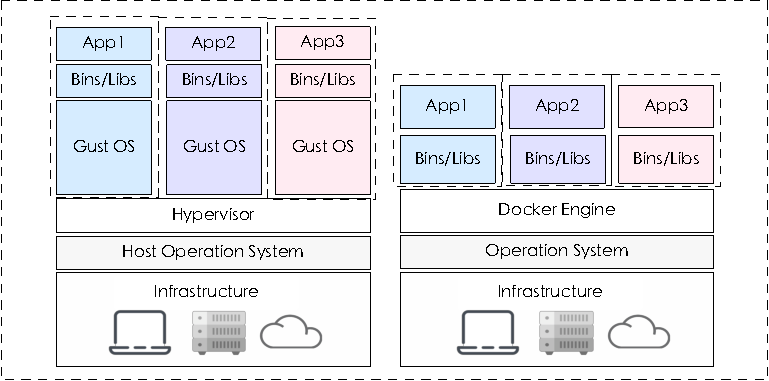
\includegraphics{docker-structure}
	\caption{容器与虚拟机对比}
	\label{fig:xfig1}
\end{figure}
图2-1中基础设施Infrastructure可以是个人电脑、服务器、云主机等,主机操作系统是运行在基础设施上的系统,最主要的是Linux各种版本,虚拟机管理系统(Hypervisor)可以实现在主机操作系统上独立运行多个子操作系统,在子操作系统上安装完应用所需的各种依赖后就可以实现资源应用的隔离。相对于虚拟机,Docker要简便很多,当前所有的Linux版本以及MacOS、Windows都能运行Docker,Docker Engine取代了Hypervisor,负载管理Docker容器并与操作系统通信,各种应用直接打包到镜像文件中,实现容器间的隔离。

对比Docker和虚拟机的架构发现,Docker直接通过守护进程与操作系统进行通信,管理容器并进行资源分配,实现容器与主操作系统的隔离。没有臃肿的子操作系统,各容器直接与主操作系统共享资源,节约了大量的磁盘空间,其虚拟化开销极大缩小,应用启动时间甚至达到毫秒级,用户可以快速构建、部署和交付应用,并且具有较强的跨平台性。
虽然Docker具有如此多的优势,但其隔离仅仅是在进程层面进行,并不能完全隔离整个运行环境。因此,用户需要根据自己的实际应用场景,需要彻底隔离用户的需求下选择虚拟机技术,如果仅是应用层面的隔离可以选择容器,如数据库、前端、后端等。
\subsection{OpenShift容器云平台}
\label{chap1:sample:table} 
Docker是当前主流的容器技术代表,Kubernetes作为现阶段应用最为广泛的容器编排引擎,OpenShift将这两种主流技术应用于企业,作为红帽公司提供的一款开源容器云平台。
该平台底层以Docker作为容器引擎驱动,Kubernetes作为容器编排组件,对外提供多种开发语言、中间件、数据库以及极易操作的用户界面、DevOps(Development and Operations)工具等。允许开发者和开发团队在该平台上进行应用的构建、测试、部署以及发布,是一套完整的容器应用云平台。在该平台上可以运行和支持有状态和无状态的应用;为容器应用提供较强的安全防护,包括基于用户的访问控制、检查机制以及强制隔离措施;实现多种综合云原生服务,便于快速智能、灵活开发应用、构建各种分布式系统;支持多种云环境包括Amazon Web Service、Azure、Google云平台以及VMware等;为开发运维团队提供一个通用的平台和工具,保持持续的开发和测试。OpenShift分为开源的社区版OpenShift Origin和收费的企业版OpenShift Enterprise,本文实验主要在开源的OpenShift Origin上进行分析和测试。
从技术堆栈的角度分析,OpenShift自下而上可以划分为基层架构层、容器引擎层、容器编排层、PaaS服务层、界面及工具层,如图2.2所示。下面分别对这几个层次进行介绍:
\begin{enumerate}[1.]
	\item 基础架构层。OpenShift运行所需的基础设施和环境,包括物理机、云主机、虚拟机、各种公有云、私有云以及混合云等。OpenShift支持多种操作系统,如CentOS7以上、Fedora21、Red Hat Enterprise Linux等,最后专门针对Atomic Host进行支持,是对企业版的Linux进行定制和优化的操作系统,可以为应用提供高度一致的运行环境,保证集群的稳定和安全。容器应用虽然具有较强的夸平台型,其前提是要求底层操作系统的内核和配置必须一致,因为其隔离依赖于Linux的内核。
	\item 容器引擎层。以当前主流的Docker作为OpenShift容器引擎,Docker已广泛应用于各种社区和环境中,经过了安全、稳定和高可用的检验。OpenShift并未修改任何原生的Docker代码,所有的应用最终到底层都生成一个Docker实例,只是将Docker的开放性和大量的镜像文件无缝衔接到平台上,对Docker的普通用户可以快速整合到平台中。
	\item 容器编排层。容器的编排对容器云的性能和资源利用效率具有决定性作用,OpenShift最终选择开源轻量的Kubernetes作为其容器编排引擎,Kubernetes已在Google内部使用多年,其诞生初衷就是为解决大规模集群中容器的调度和管理问题。OpenShift平台中很多基本的概念如Namespace、Pod、Replication Controller等都继承自Kubernetes,OpenShift同样只是将Kubernetes进行叠加使用,并未修改其原生代码和对象,用户依然可以通过原生的命令操作Kubernetes的对象。
	\item PaaS服务层。OpenShift在PaaS服务层提供了多种开发语言、框架、数据库以及中间件,极大提升了上层应用的开发、部署和交付速度。OpenShift有一个专门的社区以及Docker Hub提供各种应用的镜像,用户可以快速获取一个应用的基本镜像,构建自己所需的环,Red Hat的JBoss中间件几乎全部实现了容器化。
	\item 界面及工具层。OpenShift平台强大的界面及工具极大帮助普通用户高效完成相关应用业务,用户可以通过Web进行鼠标操作,平台将自动从Docker Hub中拉取所需的镜像进行应用构建,全自动化的服务极大降低了运维成本和提升服务效率。此外,OpenShift平台还提供S2I(Source to Image)服务,用户开发完成后可以自动整合到镜像中,快速实现交付,提升开发、测试、部署效率。针对用户端接入问题,平台提供Web控制台、IDE集成、命令行工具、以及RESTful API编程接口,用户可以最大限度的自由发挥。
\end{enumerate}
\begin{figure}[H] % use float package if you want it here
	\centering
	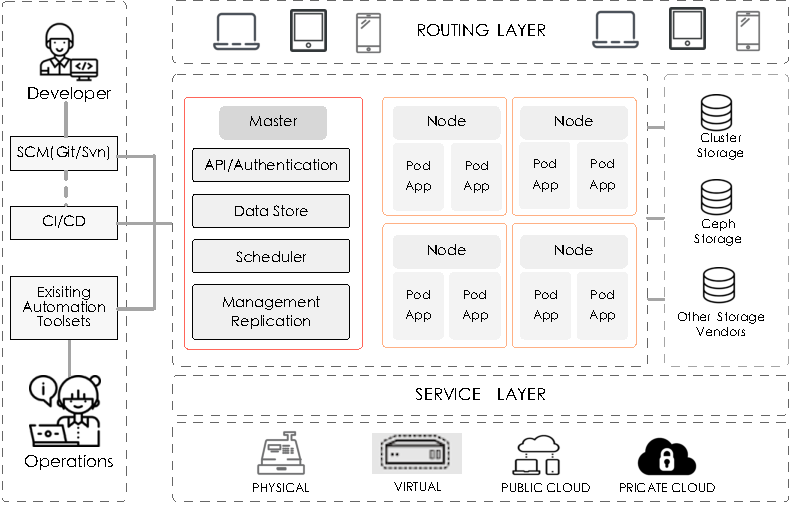
\includegraphics{openshift-structure}
	\caption{OpenShift Origin架构图}
	\label{fig:xfig1}
\end{figure}

如图2.2所示,OpenShift平台的核心组件包括Master、Node、Pod、Scheduler、Service、Storage等。Mater是主控节点,可以配置高可用的多个主控节点,负责管理和维护OpenShift集群的状态。Master上运行的API Server是其核心组件,所有用户的Web Console以及RESTful API服务都通过该组件进行访问认证控制,各Node节点也会定期轮询API Server更新其状态和容器的状态。Data Store将所有的状态信息存储在分布式的数据库Etcd中,并通过ceph一致性协议保证其数据的一致性,Etcd可以安装在主控节点,也可以单独安装到集群之外。Scheduler调度控制器进行Pod资源的分配和调度,收集过各节点资源情况,选择最优的节点作为容器应用的调度目标。Replication Controller异常自检测和恢复组件,负责监控集群中容器应用的状态和数量是否和用户要求一致,自启动和关闭容器应用满足用户的需求。Node节点通过接收Master节点指令维护容器应用。Pod是OpenShift平台调度器调度的最小单元,一些容器应用和应用之间往往存在较大的关联性,将几个联系紧密的容器部署在一个Pod中进行调度,提升应用的效率,如分布式数据库。容器是一个非持久化的对象,一旦容器重启或销毁,其状态信息将会随之销毁,集群每次给Pod分配的IP地址不同,要对外提供统一持久的服务,需要Service组件,该组件能将所有的信息转发到其对应的容器IP和端口上。此外,还有Router、Persistent Storage、Registry、Haproxy、Kubelet等都是集群的重要组成组件。数据的持久化存储可以是集群的数据库、分布式数据库或者其他的数据库中,当前支持的有NFS、Ceph RDB、GlusterFS等。

\section{容器集群资源调度系统}
\label{sec:scheduler}
Docker容器技术是容器集群的核心技术,但一个高效且强大的容器编排引擎也是集群的重要组成部分。一个好的调度器既要提现出作业调度的“公平”性,同时兼顾其性能和鲁棒性,要能应用的实际的生产环境中。在集群数据中心,可以通过应用对资源的需求感知用户部署的应用类型,通常可以划分为CPU密集、内存密集、I/O密集和网络带宽密集型应用。在集群上通常是多种密集型应用同时部署和运行,调度器如何进行资源分配至关重要,这就使得调度变得异常复杂和困难,往往不存在最优解决方案。传统虚拟机的云计算中心资源调度已有相当多的研究,针对容器集群,各大容器产生也相继推出了几款优秀的容器编排引擎,根据其调度架构的不同可以划分为一体式调度系统、两层调度系统、共享状态调度系统。其代表分别是Docker公司的Swarm、Apache的Mesos、Google的Kubernetes。

\subsection{一体式调度系统}
一体式的调度使用单一的调度代理处理所有的请求,通过固定的调度算法调度所有的作业,这种调度方式导致调度扩展性很差,用户很难灵活定制自己的调度策略,而且所有的调度信息在单节点上进行运算,不能并行执行,单节点也会成为其瓶颈。Docker公司2014年发布的容器编排管理工具Swarm是典型的一体式调度系统,同期发布的还有Docker管理工具Machine以及Compose,合称为Docker三剑客。Swarm支持Docker标准的API,内置于Docker CLI中,无需进行安装,拥有活跃的社区,易于搭建并且已应用于实际的生产环境中。
\begin{figure}[H] % use float package if you want it here
	\centering
	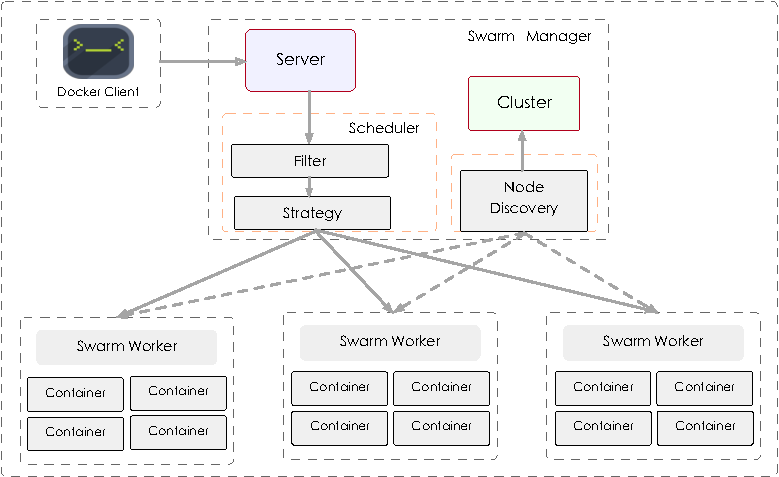
\includegraphics{swarm-structure}
	\caption{Swarm架构图}
	\label{fig:xfig1}
\end{figure}

Swarm集群由管理节点和工作节点构成,其中管理节点可以配置多个,实现高可用的多管理模式,内部通过RAFT算法实现主从的一致性。管理节点上除Docker Daemon守护进程、Load Balancing、Scaling组件外,最为重要的是Scheduler和Discovery组件,其中Discovery负责集群中节点的发现和状态更新,Scheduler首先根据用户的限制对节点进行筛选,然后使用内置的调度策略进行应用调度。工作节点主要运行Docker Daemon和Load Balancing,根据控制节点的指令运行调度过来的容器应用。在调度器的过滤模块主要提供了约束过滤器和健康过滤器,此外还可以配置吸引力过滤器、依赖过滤器和端口过滤器。

约束过滤器是通过有用的约束条件筛选节点,集群中每个节点都带有一个key-value标签,对于一些特殊的应用可以指定其label进行调度到指定的节点上运行;健康过滤器过滤掉不健康的节点,避免容器调度后运行失败;吸引力过滤器是将新的容器链接到已经创建的容器上,实现共同运行和销毁,此外还可以通过镜像和标签吸引,镜像吸引是将容器直接调度到拥有该镜像的节点上,避免重复开销镜像下载时间,节约网络资源,标签吸引是通过标签指定链接到已创建的旧容器实现共同工作;依赖过滤器是新容器依赖于其他的容器,可能会共享磁盘卷、或在同一个网络栈上等;端口过滤器将需要特定开发端口的容器运行到开放该端口的节点上,避免容器不可用的情况发生。

Swarm的调度策略主要包括Random、Spread和Binpack算法,下面分别对其算法进行简单的介绍:
\begin{enumerate}[1.]
	\item Random算法。该算法随机从过滤完的节点中选取一个节点进行调度判断,如果该节点满足条件则将容器调度到该节点上,否则随机选取下一个节点直至找到合适的节点调度,直至找到合适的节点或返回调度错误信息。
	\item Spread算法也就是最少容器算法,该算法的初衷是保证容器进群的负载均衡。每次遍历一遍集群中每个节点上运行的容器数量,选择容器数量最少的节点进行容器调度,若该节点不满足条件,则依次从后往前进行调度尝试,直至找到满足条件的节点或返回调度错误。
	\item Binpack算法就是最多容器算法,该算法的目的在于最大化利用集群中节点资源,和Spread算法相反,每次从集群中选择运行容器数量最多的节点进行容器调度,若满足条件则将容器调度至该节点,否则依次从多到少尝试运行容器节点,直至找到合适节点或返回错误。
\end{enumerate}

\subsection{两层调度系统}
两层调度系统是将资源调度和作业调度分开,资源调度层只负责给计算框架分配所需的资源,具体的作业调度由每个计算框架的调度算法完成。在一些成熟的计算处理框架中如Hadoop、Spark、MPI等有相对成熟和高效的调度算法,两层调度将这些调度算法集成进来,通过一个轻量的资源共方式来控制资源的分配和访问,一旦资源分配给某个计算框架,其他计算框架不能使用该资源,因此也会造成资源利用效率不高。Apache Mesos是最为典型的两层调度系统,Mesos最初由加州伯克利分校的AMPLab开发,后在Twitter得到广泛使用和检验。

\begin{figure}[H] % use float package if you want it here
	\centering
	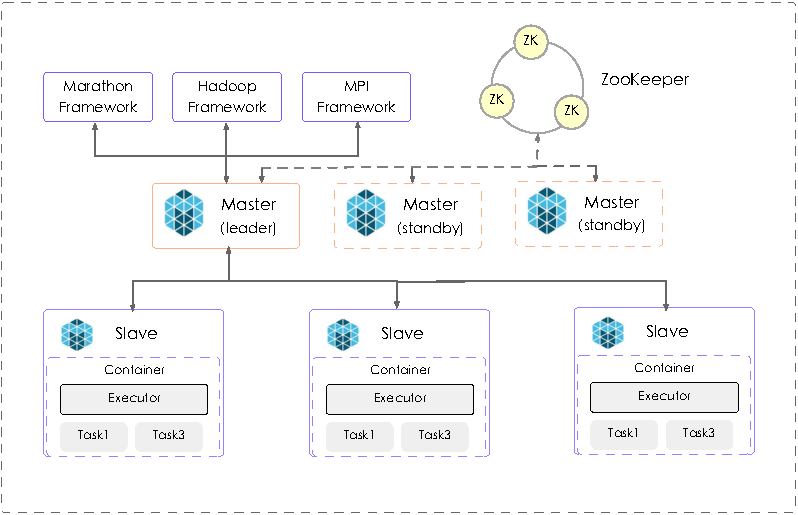
\includegraphics{mesos-structure}
	\caption{Apache Mesos架构图}
	\label{fig:xfig1}
\end{figure}

如图2.4所示,Mesos的总体架构也采用主从设计,Master节点运行作为集群的管理控制节点,可以有一个或者多个(最好为单数),为了防止单节点故障,通过ZooKeeper提供一致性服务。每次在多个Master中选举一个作为leader对外提供服务,其他的Master副本随时保证和Master的状态一直,一旦服务出现故障,立马进行新的备份选举,从而实现集群的高可用性。集群的架构可以分为两层: 计算框架层和Master调度层。下层的Master管理众多的计算节点,负责收集各节点的资源情况并作出分配决定,上层的计算框架层负责实际任务的调度,从而将整个调度分为了任务调度层和资源调度层,两个层级互不干扰,可以分别使用调度算法,提升了集群调度策略的扩展性。从架构的组成部分来看,主要有五大组成部分,下面分别对组成部分的功能进行介绍:
\begin{enumerate}[1.]
	\item ZooKeeper组件。ZooKeeper作为一款Hadoop项目中分布式系统的协调系统,主要用于解决分布式应用中数据管理问题,如应用配置管理、统一命名服务、状态同步服务以及其他的组服务、集群管理等。ZooKeeper操作非常简单易用、功能丰富可靠、并且提供了通用协议下的开源共享的存储库,其核心就是一个精简的文件系统,可以提供一些简单和抽象的操作。在Mesos中、ZooKeeper主要解决Master节点的状态一致性和高可用问题,实现集群的持续稳定的对外服务。
	\item Mesos Master组件。Master是整个集群的控制器,是整个集群调度的核心组件,既需要对底层的各Slave节点的资源进行管理和收集,同时通过一定的资源分配策略提供资源个体上层的各处理框架Framework。当前对各Framework的资源分配策略为DRF(Dominant Resource Fairness)算法,这是一种针对多维资源(CPU、内存、I/O、网络带宽等)不同需求设计的公平调度算法
	。Master还负责资源的访问控制,一旦某个资源分配给了特定的Framework,必须等该框架释放该资源才能再次进行分配。
	\item Mesos Slave组件。该组件作为调度底层具体的执行者,接收来自Master的指令,将自身的资源分配给每个执行器,执行器上运行一个或多个任务,并将各任务作为容器运行起来。
	此外,Slave节点还定期向Master节点汇报资源使用情况作为Master调度器的调度依据。Slave上还运行一个containerizer用来管理容器的生命周期的包括容器的创建、更新、监控和销毁。
	\item Framework组件。Framework负责将各计算框架如Hadoop、Spark、MPI等注册接入到集群中,Master的调度器负责对其需要的资源进行分配,具体的任务调度则由各计算框架完成。
	各计算框架通过调用Master的API进行任务的创建和调度请求,Master再将任务下发到Slave上具体执行。
	\item Executor组件。Executor负责启动框架内部的Task任务,各种计算框架接入Mesos的方式,接口不同,因此要接入一个新的计算框架就需要编写一个新的Executor,用来通知Mesos如何启动框架中的Task任务。
\end{enumerate}

Mesos作为一款优秀的分布式资源管理框架,采用双层调度机制,资源分配层负责将资源分配给计算框架,计算框架使用自身的任务调度器执行任务的调度。通过对其整体建构和核心组件的分析,Mesos可以对分布式集群的资源进行细粒度的划分,按照计算框架实际任务的需求进行资源分配,极大提升了资源的利用效率。Mesos不需要清楚各Framework的具体调度逻辑,只需要通过API向上提供资源分配即可,具有较强的扩展性,容量不会成为制约其性能的因素。Meso是模块化的实现,新增一个Framework不需要对Mesos进行重新编码,可以快速接入和扩展新的应用,Master节点使用ZooKeeper保证其状态一致性,容错性很好。但是,Mesos对底层的资源采用“悲观锁”的方式进行控制,一旦被某个Framework占用,必须等到其释放才能进行新的资源分配,其并发性受到极大的限制,独立的调度框架只能访问集群部分状态信息,往往不能实现优化调度。
\subsection{共享状态调度系统}
在一体式调度系统中,资源分配和任务调度都由中心调度器进行管理,并且集成了具体的调度算法;在两层调度系统中,资源分配由资源调度层完成,任务调度由具体的计算框架自己完成。一体式的调度很好的保证了全局状态的一致性,但是扩展性较差,两层调度系统虽然扩展性姮好,但是集群状态的一致性较难保证,并且容易造成资源的竞争和死锁。为了解决这些不足,共享状态调度系统被提了出来,其核心在于所有的调度逻辑共享集群状态,选择最优的节点进行资源分配和任务调度。其中最为典型就是Google推出的Borg、Kubernetes以及使用事务方式解决一致性管理问题的Omega,其中Kubernetes以其开源性深受大众好评,各大主流的互联公司都加大对其支持力度。

\begin{figure}[H] % use float package if you want it here
	\centering
	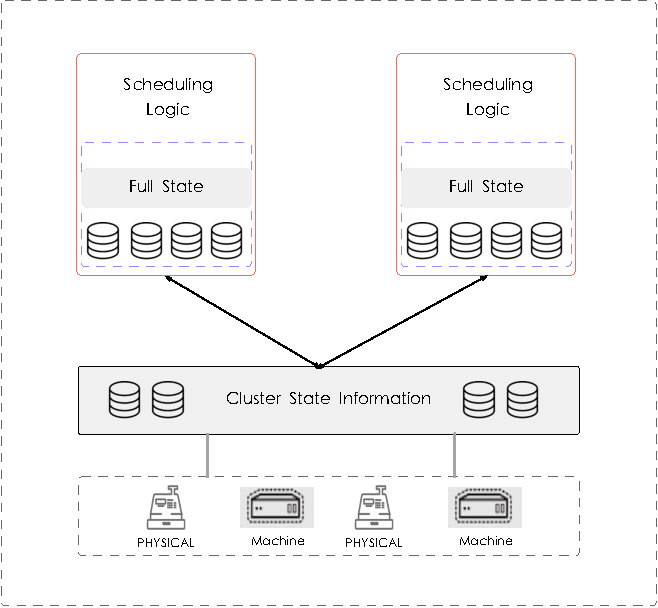
\includegraphics{full-state-structure}
	\caption{共享状态资源调度系统}
	\label{fig:xfig1}
\end{figure}
在共享状态调度系统中,每一个上层的调度器都可以对整个集群的状态进行访问,资源对所有的调度器都是透明的,可以实现自由竞争,不存在单一的资源分配器,因此也不存在单一节点访问瓶颈。集群不仅支持节点资源的快速增加,也支持调度器的扩展,用户根据自己的实际应用场景开发特殊的调度器,可以很轻易的集成到集群中。为了保证集群的高并发性和可扩展性,共享状态调度系统采用“乐观锁”对底层资源进行并发控制。具体的实现是通过对集群的所有状态都增加一个版本属性,每次提交时比较提交的版本和当前版本号大小,若版本号小于当前的版本号,则不进行任何处理,只有提交版本号大于当前数据版本号的操作才被接受,更新完状态后版本号递增。“乐观锁”并发控制虽然会增加资源访问的冲突数,影响系统的吞吐率,但在实际的系统中依然在一个可以接受范围,下一个小节将对Kubernetes调度系统架构和流程做详细的分析。

\section{Kubernetes资源调度系统}
\label{sec:bib}
Kubernetes是典型的基于共享状态的调度系统,是一个轻量的开源平台,用于容器化应用管理和服务,使用Label和Pod的概念将容器划分为逻辑单元,将相关容器进行共同调度和部署。针对其核心组件和整体架构进行深入的分析,尤其是对其调度算法和不足进行研究,为下一步提出新的调度方案提供依据。
\subsection{Kubernetes简介}
Kubernetes源自Google的Borg项目,Borg是Google集群管理工具,稳定地管理全球上百万台服务器多年。为了在容器云竞争中占据领导地位,Google基于Borg的管理经验,研发了基于Docker的容器编排工具Kubernetes,并在2014年将其开源,逐步形成一个大的生态。作为一个跨主机的应用容器编排引擎,Kubernetes提供了一系列完整的功能,包括应用部署运行、资源调度、服务发现、动态扩容以及错误恢复等。Kubernetes同时具备强大的集群管理能支撑分布式系统,实现了多租户应用、服务发现和服务注册、负载均衡、故障自处理和恢复、在线扩容、细粒度调度、资源配额管理等功能,完整定义了构建业务系统的标准化架构层。除集群管理方面的强大功能外,Kubernetes还提供完整的开发、测试、部署、运维监控在内各个环节的工具。

Kubernetes逐步发展成一个巨大生态圈,为容器的编排提供一个简单、轻量的方式,最重要的是用户可以开源定制。当前支持采用Kubernetes的云计算服务商和用户越来越多,如微软、Yahoo、IBM、华为、VMware、网易、阿里、华为、亚新等,甚至一些初创公司灵雀云、青云等都采用Kubernetes作为容器云的管理系统。

Kubernetes拥有强大而活跃的社区,众多开发者不断对其进行迭代更新,其代码更加完善。当前支持Kubernetes社区的支持者有Google、CoreOS、RedHat、华为、网易、阿里云、浙大SEL实验等。Google在2015年联合其他20多家公司成立了开源组织CNCF(Cloud Native Computing Foundation),加入OpenStack社区,力推Kubernetes的广泛应用,支持其在当前公有云、私有云等各种基础设施平台上运行,提供更加简便丰富的工具集,更好的服务用户。

\subsection{Kubernetes架构和组件}
Kubernetes是一个主从架构体系,该集群管理器很好的解决了扩容和升级两大难题,具有较强的横向扩展能力,下面展示其整体的架构体系。
\begin{figure}[H] % use float package if you want it here
	\centering
	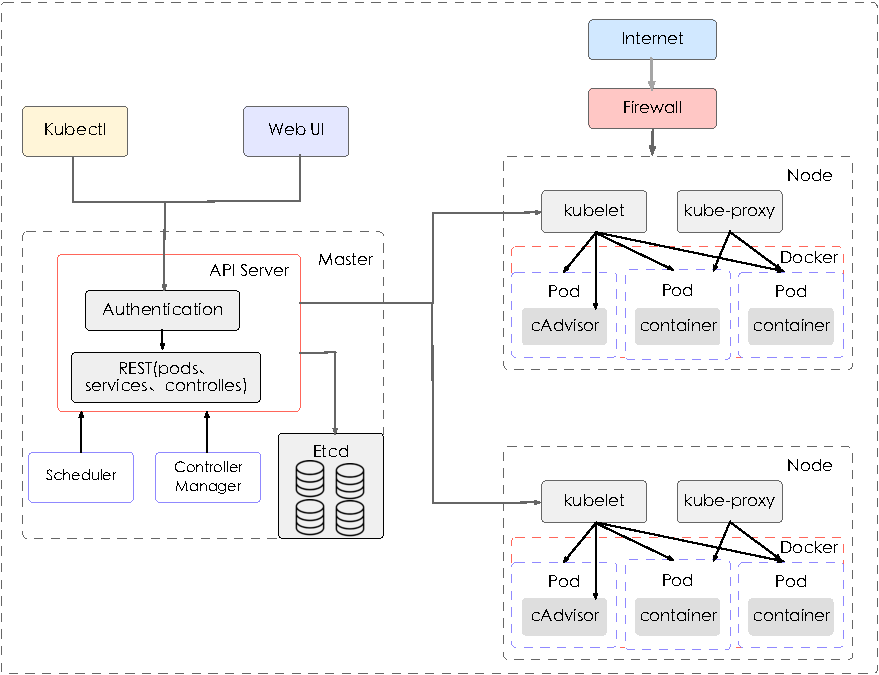
\includegraphics{kubernetes-structure}
	\caption{Kubernetes体系架构图}
	\label{fig:xfig1}
\end{figure}
如图2.6所示,Kubernetes主从架构主要由控制节点Master、工作节点Node以及外部工具集kubectl、web UI等附加依赖组成。Master作为集群的控制节点,主要负责集群的管理调度,由API Server、Scheduler、Etcd、Controller Manager等组成,实现其主要功能。Node节点主要根据控制节点的指令执行具体的任务,实现应用容器的运行,主要由kubelet、kube-proxy、cAdvisor、Container Runtime等组成。外部可以通过kubectl命令工具对集群进行增删查改的操作,也可以使用Web UI与集群进行交互。下面对集群中的重要组件分别进行介绍:
\begin{enumerate}[1.]
	\item  API Server组件。API Server是系统管理指令的统一入口,负责对外提供RESTful的API服务功能,所有对集群的操作都需要通过API Server组件进行交互,是集群外部和内部的通信枢纽中心,同时也是资源配额限制的入口,通过Authentication提供集群完备的安全认证机制。API Server接收外部Web browser或kubectl的命令请求,将REST对象持久化到Etcd中存储,同时和Node节点上的kubelet进行交互。
	\item Scheduler组件。集群调度组件,负责集群资源调度和Pod分配工作,Scheduler监控集群中未分配的Pod,根据其对资源的约束条件和集群资源可用性,将Pod调度到实际的Node上运行。这是一个可插拔的模块,用户可以开发自己的调度器集成到集群中,其调度流程和调度策略羡慕会详细的介绍。
	\item Controller Manager组件。控制管理器提供服务发现、集群管理、Pod扩容、服务绑定、应用生命周期管理等功能。主要有Node Controller用于管理节点、Replication Controller用于应用容器管理,保证容器副本和需求一致、Namespace Controller用于命名空间管理、Service Controller提供负载和服务代理、Persistent Controller管理维护Persistent Volume和Persistent Volume Claim等。
	\item Etcd组件。一个高可用、强一致性的服务发现键值存储仓库,用于保存集群中所有的网络配置和对象的状态信息,是一个中心数据库的地位,进行分布式的部署,通过watch机制进行服务更新支持。
	\item Kubelet组件。Kubelet是运行在Node节点上的控制器,用于裁决和驱动容器的执行层,是API Server和Pod的主要实现者。单个Pod中可以运行多个容器和存储数据卷,能够将Pod和相关的依赖项很方便地打包迁移,	API Server进行访问控制,Scheduler进行资源的调度,但是最终Pod能否在Node上运行成功是由kubelet决定的。此外,kubelet通过cAdvisor组件对Node节点的状态、资源进行监控,定期汇报给控制节点,存储在Etcd中。
	\item Kube-Proxy组件。负责负载均衡和反向代理组件,通过创建Pod的代理服务,用户可以通过IP地址直接访问Pod应用,实现服务到Pod的路由和转发。此外,kube-proxy还实现了一个高可用的负载均衡解决方案,
\end{enumerate}

除上述给出的核心组件外,Kubernetes还有负责提供集群DNS服务的kube-dns、提供外网访问入口的Ingress Controller、提供资源监控的Heapster、提供管理控制界面的Dashboard、提供日志采集、存储和查询的Fluentd-elasticsearch组件等。

\subsection{Kubernetes调度流程}
Kubernetes调度器运行在Master节点上,作为一个可插拔的模块,在默认配置下,调度器可以满足大部分的需求,如特定的Pod分配到到指定的节点,相同集合下的Pod分配到不同节点,平衡各节点的资源使用率等。
\begin{figure}[H] % use float package if you want it here
	\centering
	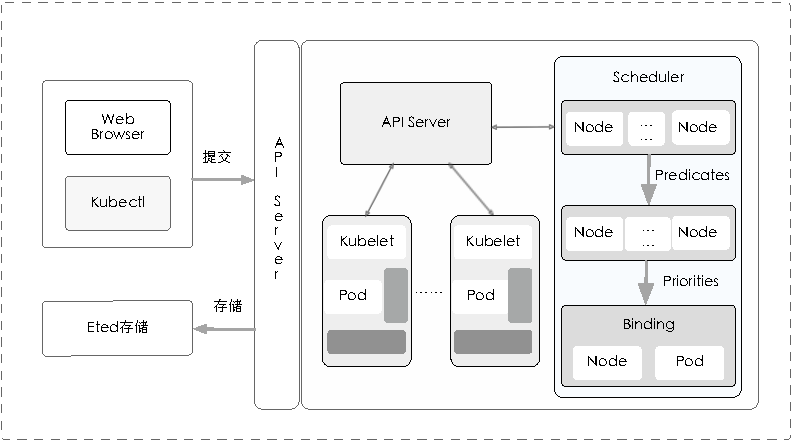
\includegraphics{kubernetes-scheduler}
	\caption{kubernetes调度流程}
	\label{fig:xfig1}
\end{figure}
调度器相对于普通用户而言类似一个黑盒,输入Pod的资源需求,输出Pod和节点的绑定,起到指挥中枢的作用。但是在很多业务场景下,用户希望自己的Pod调度可控,如制定调度算法、特殊的硬件需求的Pod调度到特殊的节点、通信量大的计算框架部署在相同机架上、数据需求大的Pod部署在存储数据的节点上等。调度器的调度流程如图2.7所示,命令工具Kubectl或Web Browser向Master上的API Server发送调度请求如创建Pod,API Server对请求做出响应处理并将处理的结果存储在Etcd中,同时设置PodSpec.NodeName为空,加入未调度Pod队列。调度器监控Etcd中未调度Pod队列状态,发现有未调度的Pod时通过调度策略尝试绑定Pod到节点,调度策略分为两个阶段: 预选阶段和优选阶段。预选阶段主要过滤节点,筛选满足Pod资源需求的节点如CPU、内存是否满足需求,端口是否冲突以及其他特定需求等,淘汰不满足需求的节点。优选阶段将满足资源需求的节点进行综合评分,主要根据资源使用的均衡性、相同副本的容灾性等调度策略,最终选取得分最高的节点,将Pod调度到该节点上,并将绑定状态存储到Etcd中。节点上的Kubelet监控Etcd中Pod调度结果,接管调度的后续工作,负责Pod生命周期的管理,一个完整的调度结束。

\section{本章小结}
本章从Docker的基本概念出发,简要阐述Docker虚拟化技术底层实现的部分原理,详细对比Docker虚拟化和虚拟机的区别以及两种技术的优缺点。接着详细介绍了集成当前流行的Docker和容器编排引擎Kubernetes技术的Openshfit Origin容器云平台的技术架构,对其重要的技术层次和核心组件进行分析,从而引发对容器编排技术的讨论。针对当前流行的三种容器编排引擎架构一体式调度、两层调度和共享状态调度进行介绍和分析,分别以Swarm、Mesos和Kubernetes为例进行深入的分析,Swarm和Mesos讨论了其核心组件和整体技术架构,由于OpenShift Origin平台采用Kubernetes作为容器编排引擎,因此,针对Kubernetes除进行核心组件介绍外,还深入盐焗了其调度流程。为下一章在OpenShift Origin容器应用平台上提出针对多计算框架的调度方案奠定基础。





\chapter{改进OpenShift Origin平台调度策略}
\label{cha:openshift}
Kubernetes作为OpenShift Origin容器云平台的容器编排引擎,其默认配置的调度算法虽能满足大部分用户需求,但其算法较为简单,集群资源利用率较低,也不能满足用户的在特定场景下的调度。本章在深入分析默认调度算法后,提出设计了一种新的基于多维资源空闲率权重的评价函数和调度方案MRWS (Multidimensional Resource WeightSscheduling)。

\section{优化Kubernetes调度流程}
Kubernetes调度算法分为预选和优选两阶段,在预选阶段过滤掉不满足需求的节点,优选阶段对剩余节点评分,选择评分最高的节点作为调度目标。整个调度器可以分为待调度的Pod列表、满足条件的Node列表以及调度策略三部分。用户除开发特殊的调度算法外,还可以针对其调度流程进行适当的优化。

\subsection{Default调度算法流程}
在Kubernetes默认调度流程,预选阶段解决节点过滤,优选阶段解决最优节点选择问题,用户可以对两个阶段进行简单的配置,调度器将根据用户指定的预选和优选规则进行过滤和评分计算,最终输出满足条件的Node和Pod绑定策略,将Pod调度到Node节点上,针对两阶段的规则,下面做详细的介绍。
\begin{figure}[H] % use float package if you want it here
	\centering
	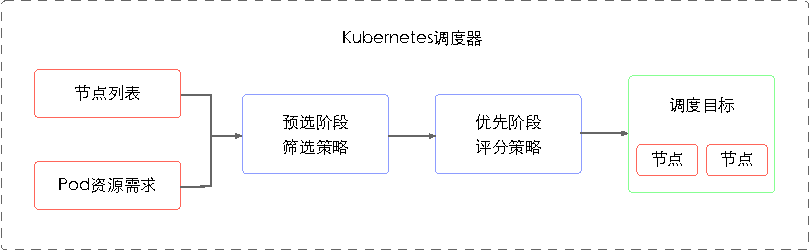
\includegraphics{scheduler-default}
	\caption{Default调度算法流程}
	\label{fig:xfig1}
\end{figure}
Predicates策略过滤掉不满足Pod需求的节点,主要依据磁盘卷是否冲突、端口冲突、资源容量、节点检测、服务占用、亲和性筛选等条件。1.7版本的筛选条件主要如下,新的版本Kubernetes还在不断完善和更新:
\begin{enumerate}[(1)]
	\item NoDiskConflict:检测卷冲突,在当前的规则中,两个不同Pod不能使用相同的卷此一旦Node上已经挂载了该卷并被某个Pod使用,则新的Pod不能再调度到该Node上,否则造成卷冲突。不同的系统对该冲突检测范围不同,如Google Compute Engine在只读模式下允许多个卷,Ceph RDB允许两个Pod分享部分资源,Amazon EBS禁止两个Pod挂载同一个卷。
	\item NoVolumeZoneConflict:在给定Zone限制的条件下,检测Node上部署的Pod是否存在卷冲突,当前只限定对PV(PersistantVolume)范围进行支持。
	\item PodFitsHostPorts:端口冲突和服务占用检测,需要调度的Pod内所有的容器需要的端口在Node上是否被其他Pod占用。
	\item PodFitsResources:根据Pod资源的需求检测节点空闲资源量是否满足其运行需求,主要检测CPU、内存、磁盘等资源。Kubernetes的调度是静态调度,资源的判断是根据分配的资源量而不是资源的实际使用量。
	\item HostName:检测Pod是否指定了Node节点,所有不在制定Node集合内的节点都将被过滤掉。
	\item MatchNodeSelector:检测Pod是否指定了MatchNodeSelector属性,若指定了该属性,Node的Label必须和该属性匹配。
	\item MaxEBSVolumeCount:确保挂载的EBS存储卷总合不超过设置最大值,调度器计算每个Node上直接或间接使用的全部卷总合,一旦超过最大值,Pod不能调度到该节点上。
	\item CheckNodeMemoryPressure:判断节点是否存在内存压力,若存在内存压力则标记为1,Pod只能调度到内存标记为0的节点上。
	\item CheckNodeDiskPressure:判断节点是否存在磁盘压力,若存在磁盘压力则标记为1,Pod只能调度到磁盘标记为0节点。
	\item MatchInterPodAffinity:节点的亲和性过滤,检测Pod是否和已部署的Pod存在亲和性,将有亲和性的Pod调度到相同节点。
	\item PodToleratesNodeTaints:判断将Pod调度到节点后是否满足节点容忍的条件,相同的Pod副本为了满足容灾性,一般部署到不同的Node甚至是不同的机架和数据中心。
\end{enumerate}
此外、还有转为Google Compute Engine和Amazon EBS配置的MaxGCEPDVolumeCount、MaxAzureDiskVolumeCount卷检测条件,检测节点上挂载的卷容量总合是否超过设定的最大值。

Priorities阶段根据一定的评分算法对预选出来的节点列表进行综合评分,评分依据主要包括资源空闲量、资源消耗平衡性、Pod亲和性、Pod与节点的匹配度等因素。Kubernetes使用优先函数集合进行0-10对节点进行评分,最终计算评分总合,评分越高表明Pod调度到该节点越适合,同时还可以为每一个函数设置一个权重值,主要的评分函数如下:
\begin{enumerate}[(1)]
	\item LeastRequestedPriority:根据资源空闲率计算节点得分,即节点的空闲资源与节点资源总量的比值((节点资源总量-节点上Pod的资源和-新Pod的需求)/总容量)来计算。设置CPU和内存具有相同权重,都设置为0.5,资源空闲率越大,剩余资源越多,节点的评分就越高。
	\item BalancedResourceAllocation:该函数必须联合LeastRequestedPriority一起使用,用于平衡各项资源的使用率,资源使用越均衡,节点的评分越高。Kubernetes主要对内存和CPU资源消耗进行平衡,由两者的“距离”决定分值大小,即使用10-abs(CPU空闲率-内存空闲率)*10进行计算。
	\item SelectorSpreadPriority:为了更好应对容灾和宕机风险,同属Service、Replication Controller下的Pod尽可能分散部署到不同的Node上。对于指定Zone的Pod,也要尽量分散到不同区域的主机。调度器统计各Node上相同Service、Replication Controller下的Pod,Node上Pod数量越少,评分越高。
	\item NodeAffinityPriority:设置调度器的亲和性机制,主要对节点进行精确匹配。有两种选择器匹配模式,选择器“hard"模式下设置的NodeSelector必须和节点的Label匹配,保证选择的Node是完全满足需求规则的,”soft"模式下不能完全保证百分百的匹配,但会尽量满足规则要求
	\item ImageLocalityPriority:为避免镜像的重复下载对网络和磁盘资源的重复消耗,该函数根据Pod中运行容器需要的镜像对节点进行评分,节点上存在的镜像越多,该节点评分越高。若该节点上没有所需的镜像,评分为0,镜像评分的权重可以根据镜像大小按比例决定。
	\item MostRequestedPriority:和LeastRequestedPriority相反,两者使用一个来计算评分。该函数确保使用资源越多的节点,评分越高,目的在于使用更少的服务器提供服务,节约集群资源,提升资源利用率。
	\item TaintTolerationPriority:容忍性评分函数,匹配Pod的TolerationList与节点Taint,匹配项越多,该节点的容忍性越好,从而评分越高。
	\item InterPodAffinityPriority:用于迭代WeightedPodAffinityTerm的元素计算和,若该节点同时满足亲和性设置,则将该评分加入节点的整体评分中。
	\item NodePreferAvoidPodsPriority:根据节点是否设置Anotation属性进行评分,没有设置该属性则评分为10,设置该属性并且调度的Pod正好是副本,则该节点评分为0,目的在于避免相同副本调度到同一节点。
\end{enumerate}

优先调度模块定义了一个评分函数集合,各评分函数的权重可以指定,用户根据调度依据的重要程度给各函数赋予不同的权重值,最终所有函数的评分总合就是该节点的最终得分,选择评分最高的节点作为Pod的调度目标。

\subsection{MRWS算法调度流程}
Kubernetes调度系统的Default算法核心在于优选阶段的评分函数,调度策略根据节点评分高低做出调度决策。在所有的评分函数中,除一些特殊的调度规则外,如节点亲和性、节点容忍度、节点上的镜像文件等,最为重要的是根据资源空闲率做出评分的LeastRequestedPriority和资源使用平衡性做出评分的BalancedResourceAllocation函数。这两个函数是整个评分函数集合中的核心,在其他外在规则相同的条件下,直接决定节点的评分高低。但是,这两个评分函数仅考虑了内存和CPU的空闲率和消耗平衡性,这种评分会造成节点其他维度资源消耗不均,如I/O、带宽、节点上运行的Pod数量等,一旦某个维度的资源过载,节点将不能部署更多的Pod,造成集群资源利用率低下。因此,新的调度算法MRWS将更多关注于集群CPU、内存、磁盘、网络带宽以及节点运行Pod数量的均衡性,提升集群的负载均衡和资源利用率。
\begin{figure}[H] % use float package if you want it here
	\centering
	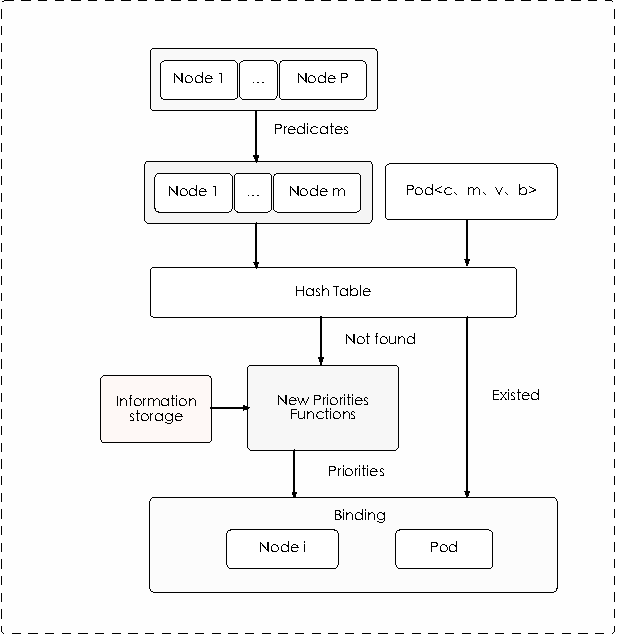
\includegraphics{scheduler-mrws}
	\caption{MRWS算法调度流程}
	\label{fig:xfig1}
\end{figure}


\subsection{插图}
\label{sec:graphs}

强烈推荐《\LaTeXe\ 插图指南》!关于子图形的使用细节请参看 \pkg{subcaption} 宏包的说明文档。

\subsubsection{一个图形}
\label{sec:onefig}
一般图形都是处在浮动环境中。之所以称为浮动是指最终排版效果图形的位置不一定与源文
件中的位置对应\footnote{This is not a bug, but a feature of \LaTeX!},这也是刚使
用 \LaTeX{} 同学可能遇到的问题。如果要强制固定浮动图形的位置,请使用 \pkg{float} 宏包,
它提供了 \texttt{[H]} 参数,比如图~\ref{fig:xfig1}。
\begin{figure}[H] % use float package if you want it here
  \centering
  
\includegraphics{thu-whole-logo}
  \caption{利用 Xfig 制图}
  \label{fig:xfig1}
\end{figure}

大学之道,在明明德,在亲民,在止于至善。知止而后有定;定而后能静;静而后能安;安
而后能虑;虑而后能得。物有本末,事有终始。知所先后,则近道矣。古之欲明明德于天
下者,先治其国;欲治其国者,先齐其家;欲齐其家者,先修其身;欲修其身者,先正其心;
欲正其心者,先诚其意;欲诚其意者,先致其知;致知在格物。物格而后知至;知至而后
意诚;意诚而后心正;心正而后身 修;身修而后家齐;家齐而后国治;国治而后天下
平。自天子以至于庶人,壹是皆以修身为本。其本乱而未治者 否矣。其所厚者薄,而其所
薄者厚,未之有也!

\hfill —— 《大学》


\subsubsection{多个图形}
\label{sec:multifig}

如果多个图形相互独立,并不共用一个图形计数器,那么
用 \texttt{minipage} 或者\texttt{parbox} 就可以。否则,请参看
图~\ref{fig:big1-subcaptionbox},它包含两个小图,分别是图~\ref{fig:subfig1}和
图~\ref{fig:subfig2}。推荐使用 \cs{subcaptionbox},因为可以像
图~\ref{fig:big1-subcaptionbox} 那样对齐子图的标题,也可以使用 \pkg{subcaption}
宏包的 \cs{subcaption}(放在 minipage中,用法同\cs{caption})或
是 \pkg{subfigure} 、\pkg{subtable}环境,像图~\ref{fig:big1-subfigure},不要再
用 \cs{subfloat}、\cs{subfigure} 和 \cs{subtable}。

\begin{figure}[h]
  \centering%
  \subcaptionbox{第一个小图形\label{fig:subfig1}}[3cm] %标题的长度,超过则会换行,如下一个小图。
    {
\includegraphics[height=3cm]{thu-fig-logo}}%
  \hspace{4em}%
  \subcaptionbox{第二个小图形,注意这个图略矮些。如果标题很长的话,它会自动换行\label{fig:subfig2}}
      {
\includegraphics[height=2cm]{thu-text-logo}}
  \caption{包含子图形的大图形(subcaptionbox示例)}
  \label{fig:big1-subcaptionbox}
\end{figure}
\begin{figure}[h]
  \centering%
  \begin{subfigure}{3cm}
    
\includegraphics[height=3cm]{thu-fig-logo}
    \caption{第一个小图形}
  \end{subfigure}%
  \hspace{4em}%
  \begin{subfigure}{0.5\textwidth}
    
\includegraphics[height=2cm]{thu-text-logo}
    \caption{第二个小图形,注意这个图略矮些。subfigure中同一行的子图在顶端对齐。}
  \end{subfigure}
  \caption{包含子图形的大图形(subfigure示例)}
  \label{fig:big1-subfigure}
\end{figure}

古之学者必有师。师者,所以传道受业解惑也。人非生而知之者,孰能无惑?惑而不从师,
其为惑也,终不解矣。生乎吾前,其闻道也固先乎吾,吾从而师之;生乎吾後,其闻道也亦
先乎吾,吾从而师之。吾师道也,夫庸知其年之先後生於吾乎!是故无贵无贱无长无少,道
之所存,师之所存也。

嗟乎!师道之不传也久矣,欲人之无惑也难矣。古之圣人,其出人也远矣,犹且从师而问焉;
今之众人,其下圣人也亦远矣,而耻学於师。是故圣益圣,愚益愚。圣人之所以为圣,愚
人之所以为愚,其皆出於此乎?爱其子,择师而教之,於其身也,则耻师焉,惑焉。彼童子
之师,授之书而习其句读者,非吾所谓传其道、解其惑者也。句读之不知,惑之不解,或师
焉,或不焉,小学而大遗,吾未见其明也。巫医、乐师、百工之人不耻相师,  士大夫之族
曰“师”曰“弟子”之云者,则群聚而笑之。问之,则曰:彼与彼年相若也,道相似也,位
卑则足羞,官盛则近谀。呜呼!师道之不复,可知矣。巫医、乐师、百工之人。吾子不齿,
今其智乃反不能及,其可怪也欤!圣人无常师。孔子师郯子、苌子、师襄、老聃。郯子之徒,
其贤不及孔子。孔子曰:“三人行,必有我师。”是故弟子不必不如师,师不必贤於弟子。
闻道有先後,术业有专攻,如是而已。

如果要把编号的两个图形并排,那么小页就非常有用了:
\begin{figure}
\begin{minipage}{0.48\textwidth}
  \centering
  
\includegraphics[height=2cm]{thu-whole-logo}
  \caption{并排第一个图}
  \label{fig:parallel1}
\end{minipage}\hfill
\begin{minipage}{0.48\textwidth}
  \centering
  
\includegraphics[height=2cm]{thu-whole-logo}
  \caption{并排第二个图}
  \label{fig:parallel2}
\end{minipage}
\end{figure}

李氏子蟠,年十七,好古文、六艺,经传皆通习之,不拘於时,学於余。余嘉其能行古
道,作师说以贻之。

\hfill —— 韩愈(唐)

\chapter{FAHP自动求解MRWS调度方法权重参数}
在上一章MRWS调度算法的评分函数中,根据资源的重要程度使用系数$\alpha_{i}(i=1,2,3,4,5), \quad\alpha_{1}+\alpha_{2}+\alpha_{3}+\alpha_{4}+\alpha_{5}=1$作为节点CPU、内存、磁盘I/O、网络带宽和已部署Pod数量的重要程度系数。本章需要对筛选后的节点和容器应用资源进行建模,并利用FAHP方法进行Pod应用多维权重参数的自动求解。

\section{模糊层次分析法FAHP}
模糊层次分析法FAHP~\cite{Kwong2002A,Hong2013Cloud}(Fuzzy Analytical Hierarchy Process)是在层次分析法的基础发展而来,常用于解决实际问题中影响决策问题的多种因素的权重。下面从层次分析法开始介绍,为弥补层次分析法的不足引入FAHP方法,然后举例说明如何使用该方法解决实际问题。

\subsection{FAHP方法介绍}
在许多实际问题中,通常有较多的解决方案,我们需要对影响方案的因素进行比较、判断、评价,然后做出方案选择,这种人为主观做出决策的方式不但效率低下,结果也不够准确。层析分析法AHP~\cite{Saaty1994How,Deng2012}(Analytical Hierarchy Process)是由著名的美国运筹学家,匹茨堡大学的T.L.Saaty教授提出的一种层次权重决策分析方法。该方法用于解决复杂的多目标决策问题,影响最终决策的因素被分解为目标层、准则层和方案层等层次,使用数学方法对各因素权重进行精确求解。层次分析法将问题的总目标、各层子目标以及决策因素分解成多个层次结构,然后构建各层次的判断矩阵,求解判断矩阵的特征值。最大特征值对应的特征向量归一化获得上一层各因素对本层目标的权重系数,然后用加权和的方法递阶归并各备选方案对总目标的最终权重,选择最大权重的备选方案作为最终的目标。该方法是一个系统性的分析方法,先将问题分解成多个层次,然后对影响子目标的因素进行比较判断、最终进行综合决策。该方法结构层次清晰、单层的权重参数设置都会影响到最终的决策层,不断分割量化各因素的影响。层次分析法非常实用,将定量分析和定性分析相结合,用于解决许多实际问题如电力分配、旅游决策等,该方法计算简单明了,易于掌握。最后,该方法用于模拟人们解决问题的思维,所需的定量信息较少,仅需要对影响决策因素的重要性做出判断即可。

但是,层次分析法也具有较大的局限性,在一些场景下效果较差甚至无法使用。首先,该方法只能从实际的备选方案中帮助决策者选出较优的决策方案,不能给决策者提供新的解决方案或者反馈合理方案的意见,并且该方法是单目标决策方法,使用者只能从备选方案中选出一个较优的目标。其次,该方法模拟人类大脑决策过程,过于依赖于定性分析,只能进行粗略比较计算,不能完全做到精确模拟。最后,从层次结构转化为成对比矩阵过程中,判断者的主观因素影响过大,使用者不同,得出的最优方案也不尽相同,可重复性较差。并且随着影响决策因素的增加,构建的成对比矩阵阶数增大,计算难度和复杂度随之增加,很难一次性构建出满足一致性要求的成对比矩阵。

为减少人为主观因素对决策结果的影响,模糊层析分析法FAHP在层次分析法的基础上增加人为判断的模糊性。层析分析是通过两两比较构建成对比判断矩阵,而FAHP通过两两比较构建模糊成对比矩阵,提升了层次分析法解决问题的可靠性。在进行问题判断或专家咨询时,通常获得的不是一个具体值,而是一个模糊数,如三值判断(最低可能值、最可能值和最大可能值)、二值区间(上界和下界)等。下面介绍模糊数集的概念,一个明确的集合表示如下:
\begin{equation}
\mu_{A}(x) = \left\{\begin{array}{l}
1, x\in A \\ [0.3cm]
0, x\notin A
\end{array}\right.
\end{equation}
在明确的集合中,$x\in A$时值为1,$x\notin A$时值为0。但对于一个模糊数集,并不能完全明确x是否属于A,只能用[0,1]表示其隶属度。
\begin{equation}
\mu_{A}(x):U\to[0,1]
\end{equation}
\begin{math}\mu_{A}(x)\end{math}表示\begin{math}x\in A\end{math}的隶属度,也称\begin{math}\mu_{A}(x)\end{math}为集合A的隶属函数。对于任意的模糊数集,都对应一个隶属函数,隶属函数通常模仿概率论中的分布函数如正态分布、梯形分布、K次抛物线分布、S分布以及柯西分布等,值域在[0,1]上。

1983年,荷兰学者Van Loargoven首次提出用三角模糊数~\cite{Wang2010Triangular,Chou2003The}作为模糊数集的判断标准,并运用三角模糊数的运算和对数最小二乘法获取权重值。设论域R上的模糊数$\widetilde{M}$为三角模糊数,其对应的隶属函数\begin{math}\mu_{\widetilde{M}:}R\to[0,1]\end{math}满足下列函数:
\begin{equation}
\mu_{\widetilde{M}}(x) = \left\{\begin{array}{l}
0 \quad x<a \\ [0.2cm]
\frac{x-a}{b-a} \quad a\le x\le b \\ [0.2cm]
\frac{c-x}{c-b} \quad b\le x\le c \\ [0.2cm]
0 \quad x>c
\end{array}\right.
\end{equation}
$\widetilde{M}=(a,b,c) \quad a\le b\le c$,
a和c分别表示三角模糊数的上界和下界,b是隶属度为1的中间值,x=b时表示x完全属于$\widetilde{M}$,x在a和c之外的不属于模糊数$\widetilde{M}$。定义一个置信度$\alpha$可以将三元组的模糊数$\widetilde{M}$化为一个$\alpha$割集的二元形式,从而构建$\alpha$割集矩阵,设定优化参数后将二元值的矩阵转化成最终的判断矩阵。
\begin{equation}
	\widetilde{M}_{\alpha} = [l^{\alpha},u^{\alpha}]=[(b-a)\alpha+a,-(c-b)\alpha+c] \quad \forall \alpha\in[0,1]
\end{equation}
根据Arnold J. Kaufmann在文献~\inlinecite{Eastman1987Introduction}中的描述,$\alpha$割集后的基本运算规则如下:
\begin{equation}
\begin{split}
	\widetilde{M}_{\alpha} &= [m_{L}^{\alpha},m_{R}^{\alpha}] \\[0.2cm]
	\widetilde{N}_{\alpha} &= [n_{L}^{\alpha},n_{R}^{\alpha}] \\[0.2cm]
	\widetilde{M}_{\alpha}\oplus \widetilde{N}_{\alpha} &= [m_{L}^{\alpha}+n_{L}^{\alpha},m_{R}^{\alpha}+n_{R}^{\alpha}] \\[0.2cm]
	\widetilde{M}_{\alpha}\ominus \widetilde{N}_{\alpha} &= [m_{L}^{\alpha}-n_{L}^{\alpha},m_{R}^{\alpha}-n_{R}^{\alpha}] \\[0.2cm]
	\widetilde{M}_{\alpha}\otimes \widetilde{N}_{\alpha} &= [m_{L}^{\alpha}n_{L}^{\alpha},m_{R}^{\alpha}n_{R}^{\alpha}] \\[0.2cm]
	\widetilde{M}_{\alpha}\oslash \widetilde{N}_{\alpha} &= [m_{L}^{\alpha}/n_{L}^{\alpha},m_{R}^{\alpha}/n_{R}^{\alpha}] \\[0.2cm]
	\end{split}
\end{equation}
本文采用三角模糊数作为FAHP的隶属函数进行权重参数求解,并将三元组的$\widetilde{M}$=(a,b,c)转化成$\alpha$割集形式
$\widetilde{M}_{\alpha} =[(b-a)\alpha+a,-(c-b)\alpha+c] \quad \forall \alpha\in[0,1]$。

\subsection{FAHP求解权重参数步骤}
介绍完层次分析方法和模糊层析分析方法以及模糊数的基本概念后,下面用三角模糊数作为模糊程度的衡量值,FAHP求解权重参数流程如下:
\begin{figure}[H] % use float package if you want it here
	\centering
	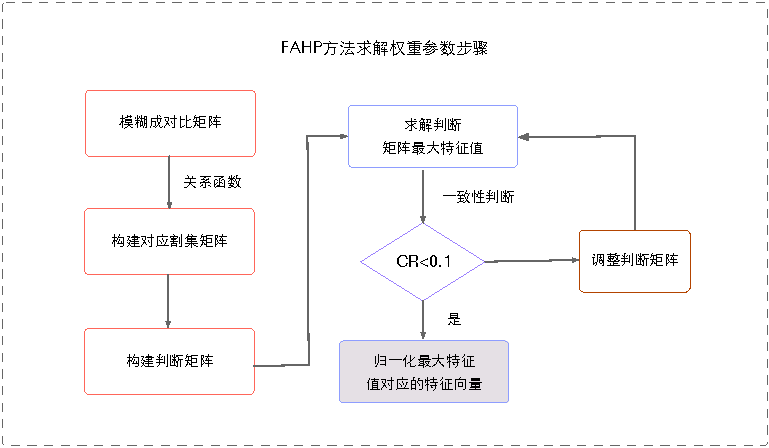
\includegraphics{fahp-flow}
	\caption{FAHP计算权重参数过程}
\end{figure}
如图4.1所示,使用FAHP方法计算权重参数的步骤可以分为构建模糊成对比矩阵、设置$\alpha$转化为$\alpha$割集矩阵、设置优化参数转化为判断矩阵,求解判断矩阵的最大特征值,检验最大特征值是否满足随机一致性比率要求。若通过检测则将最大特征值对应的特征向量归一化作为权重参数值,否则需要调整判断矩阵值,重新进行特征值计算。下面详细介绍求解步骤:

1) 构建模糊成对比矩阵。在FAHP中,对影响决策因素进行两两对比并使用$\widetilde{1}\sim \widetilde{9}$表示其相对重要程度,值越大,表示该因素相对另一个因素对决策目标的影响越大,重要性越高。模糊数、相对重要程度、$\widetilde{M}$三元组及其$\alpha$割集如表4.1所示,可以构建最终的模糊成对比矩阵$\widetilde{A} $,其中的元素$\widetilde{a}_{ij} $表示因素i相对j的重要程度,模糊成对比矩阵中元素值如式(4-6)所示。
\begin{equation}
\widetilde{a}_{ij} = \left\{\begin{array}{l}
1 \quad i=j \\ [0.2cm]
\widetilde{1},\widetilde{3},\widetilde{5},\widetilde{7},\widetilde{9}\ or\ \widetilde{1}^{-1},\widetilde{3}^{-1},\widetilde{5}^{-1},\widetilde{7}^{-1},\widetilde{9}^{-1} \quad i\not=j  
\end{array}\right.
\end{equation}
\begin{table}[htbp]
	\centering\dawu[1.3]
	\caption{模糊数、相对重要程度和$\alpha$割集关系表}
	\begin{tabular}{|c|c|c|c|c|c|} \hline
		模糊数 & $\widetilde{1}$ & $\widetilde{3}$ & $\widetilde{5}$  & $\widetilde{7}$ & $\widetilde{9}$ \\ \hline
		重要性 & 同等重要 & 稍微重要 & 重要 & 明显重要 & 非常重要 \\ \hline 
		$\widetilde{M}$ & (1,1,3) & (1,3,5) & (3,5,7) & (5,7,9) & (7,9,11) \\ \hline 
		$\widetilde{M}_{\alpha}$ & [1,3-2$\alpha$] & [1+2$\alpha$,5-2$\alpha$] & [3+2$\alpha$,7-2$\alpha$] & [5+2$\alpha$,9-2$\alpha$] & [7+2$\alpha$,11-2$\alpha$]\\ \hline 
	\end{tabular}
\end{table}

2) 构建$\alpha$割集矩阵并转化为判断矩阵。构建模糊成对比矩阵后,根据表4.1将模糊数转化成三元组的三角模糊数,给定$\alpha$后,将三元组转化成$\alpha$割集$\widetilde{M}_{\alpha}=[l_{\alpha},u_{\alpha}]$,从而构建一个$\alpha$割集矩阵$\widetilde{A}_{\alpha}$,割集矩阵中的元素$\widetilde{a}_{ij}^{\alpha}$如式(4-7)所示。给定一个优化参数表示判断优化程度,可以将二元组割集矩阵转化成判断矩阵A,A是一个方阵,接着求解判断矩阵特的征值和特征向量。设给定的优化参数$\mu\in[0,1]$,将割集矩阵中上下界范围转化成判断矩阵的单值,判断矩阵中的元素$a_{ij}=(1-\mu)l_{\alpha}+\mu u_{\alpha}$,如式(4-8)所示。通过给定$\alpha$获得二元组的割集矩阵,给定割集矩阵一个优化参数$\mu$可以得到最终的判断矩阵A。
\begin{equation}
\widetilde{a}_{ij}^{\alpha} = \left\{\begin{array}{l}
1 \quad \widetilde{a}_{ij}=1 \\ [0.2cm]
[l_{\alpha},u_{\alpha}] \quad \widetilde{a}_{ij}\in{\widetilde{1},\widetilde{3},\widetilde{5},\widetilde{7},\widetilde{9}} \\ [0.2cm]
[\frac{1}{u_{\alpha}},\frac{1}{l_{\alpha}}] \quad \widetilde{a}_{ij}\in{\widetilde{1}^{-1},\widetilde{3}^{-1},\widetilde{5}^{-1},\widetilde{7}^{-1},\widetilde{9}^{-1}}
\end{array}\right.
\end{equation}
\begin{equation}
a_{ij} = \left\{\begin{array}{l}
1 \quad \widetilde{a}_{ij}=1 \\ [0.2cm]
(1-\mu)l_{\alpha}+\mu u_{\alpha} \quad \widetilde{a}_{ij}\in{\widetilde{1},\widetilde{3},\widetilde{5},\widetilde{7},\widetilde{9}} \\ [0.2cm]
\frac{1-\mu}{u_{\alpha}}+\frac{\mu}{l_{\alpha}} \quad \widetilde{a}_{ij}\in{\widetilde{1}^{-1},\widetilde{3}^{-1},\widetilde{5}^{-1},\widetilde{7}^{-1},\widetilde{9}^{-1}}
\end{array}\right.
\end{equation}

3) 计算判断矩阵最大特征值和特征向量。对判断矩阵特征值的求解是一个纯数学问题,求解方阵特征值和特征向量的方法有几何平均法(方根法)、算术平均平均法(和法)、最小二乘法(幂法)和特征向量法。几种方法求解的特征值近似相等,但也存在细微的差别,这种细微的误差可能会影响实际生产。通常情况下,几何平均法和算术平均获得的结果精确度较差,最小二乘法计算复杂度较高,因此使用特征向量法对判断矩阵的特征值和特征向量进行求解。在本文中,直接使用Python中numpy库eig()函数求解判断矩阵的特征值和特征向量。

4) 一致性检验和归一化权重。通过特征向量法获得判断矩阵的最大特征值$\lambda_{max}$及其对应的特征向量$\nu_{max}$后,需要进行层次单排序和层次总排序的一致性检验,用于检测特征向量和真实权值的契合度,即求解的权重值是否合理。判断矩阵一致性检测方法公式如式(4-9)所示。
\begin{equation}
\begin{split}
CI &= \frac{\lambda_{max}-n}{n-1} \\
CR &= \frac{CI}{RI}
\end{split}
\end{equation}
其中,$\lambda_{max}$是判断矩阵最大特征值,n判断矩阵阶数即影响决策因素的数量,CI是一般一致性指标,RI是随机一致性指标,因此,CR是随机一致性比率。若CR<0.1时,判断矩阵满足一致性要求,否则程序自动调整判断矩阵直至满足一致性判断要求。当CR<0.1时,归一化$\lambda_{max}$对应的特征向量$\nu_{max}$,其值w就是所需求解的权重系数。n阶随机一致性指标RI的值如表4.2所示。
\begin{table}[htbp]
	\centering\dawu[1.3]
	\caption{随机一致性指标RI值}
	\begin{tabular}{|p{0.8cm}<{\centering}|p{0.8cm}<{\centering}|p{0.8cm}<{\centering}|p{0.8cm}<{\centering}|p{0.8cm}<{\centering}|p{0.8cm}<{\centering}|p{0.8cm}<{\centering}|p{0.8cm}<{\centering}|p{0.8cm}<{\centering}|p{0.8cm}<{\centering}|p{0.8cm}<{\centering}|} \hline
	n & 1 & 2 & 3 & 4 & 5 & 6 & 7 & 8 & 9 & 10 \\ \hline
	RI & 0 & 0 & 0.58 & 0.90 & 1.12 & 1.24 & 1.32 & 1.41 & 1.45 & 1.49 \\ \hline
	\end{tabular}
\end{table}

上述是用FAHP方法求解权重参数的全部过程,首先对影响决策的因素进行两两比较,构建模糊成对比矩阵,用$\widetilde{1}\sim \widetilde{9}$表示相对重要程度。针对模糊成对比矩阵,给定$\alpha\in[0,1]$获得割集矩阵,设定优化参数$\mu \in[0,1]$获得判断矩阵,对判断矩阵特征值和对应的特征向量进行求解,检测判断矩阵是随机一致性比率值是否满足要求,最大特征向量归一化获得权重系数。

\subsection{FAHP求解权重参数示例}
上一小节介绍了FAHP求解权重参数的详细流程和计算方法,下面通过一个简单的例子展示该方法求解权重参数的计算过程。假设在一个物理问题中力学指数的评价由巴氏硬度、耐荷重性、耐冲击性和满水变形四个因素决定,其影响力学指数的判断因素层次如图4.2所示。
\begin{figure}[H] % use float package if you want it here
	\centering
	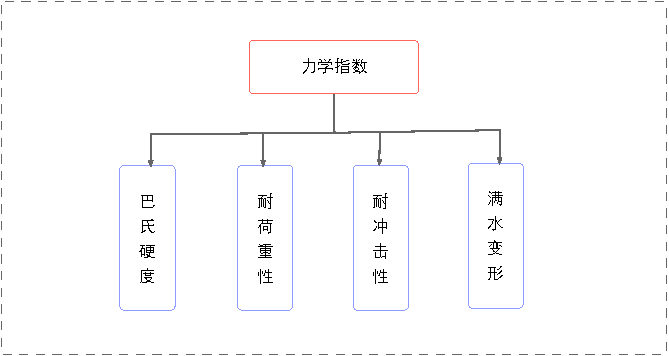
\includegraphics{fahp-example}
	\caption{力学指数的评价因素}
\end{figure}
某专家通过对影响力学指数的因素进行两两对比后给出其三角模糊判断数,根据其给出的模糊数构建模糊成对比矩阵如式(4-10),从左至右依次为巴氏硬度、耐荷重性、耐冲击性和满水变形。
\begin{equation}
\widetilde{A} = \left\{\begin{array}{cccc}
1 & \widetilde{3} & \widetilde{7} & \widetilde{5}  \\
\widetilde{3}^{-1} & 1 & \widetilde{5} & \widetilde{3} \\
\widetilde{7}^{-1} & \widetilde{5}^{-1} & 1 & \widetilde{3}^{-1} \\
\widetilde{5}^{-1} & \widetilde{3}^{-1} & \widetilde{3} & 1 \\
\end{array}\right\}
\end{equation}
给定$\alpha=0.5$和优化参数$\mu=0.5$,根据式(4-7)和(4-8)可以获得割集矩阵和判断矩阵,判断矩阵A如下:
\begin{equation}
A = \left\{\begin{array}{cccc}
1 & 3 & 7 & 5 \\
\frac{3}{8} & 1 & 5 & 3 \\
\frac{7}{48} & \frac{5}{24} & 1 & \frac{3}{8} \\
\frac{5}{24} & \frac{3}{8} & 3 & 1 \\
\end{array}\right\}
\end{equation}

使用特征向量法求解判断矩阵进行特征值和对应的特征向量,最大特征值$\lambda_{max}=4.21154$,其对应的特征向量值$\nu_{max}=[0.88297,0.41986,0.08951,0.18992]$,使用最大特征值对判断矩阵A的一致性进行判断,CR=0.082<0.1满足一致性要求。对其最大特征值对应的特征向量进行归一化,其权重w=[0.558,0.265,0.057,0.120]分别表示巴氏硬度、耐荷重性、耐冲击性和满水变形四个因素对力学系数影响的权重系数,用于对后面的目标层做出决策。

\section{容器应用多维资源权重自动求解}
上一小节详细介绍了FAHP方法求解权重系数的流程,并用一个力学系数的例子展示其计算过程。在MRWS调度算法中,需要使用容器应用各维资源的权重参数进行节点评分,由于需要调度的容器应用数量庞大,不能依赖人工给每一个容器应用的资源需求赋予一个权重值,这样既不准确也不现实。因此,下面将介绍使用FAHP方法对容器应用的多维资源进行建模并自动求解。
\subsection{容器应用多维资源建模}
在MRWS调度方法中,集群中节点CPU、内存、磁盘和网络带宽以及已部署的Pod数量作为影响容器应用调度决策的因素,预选阶段筛选后的节点作为其调度的备选节点。不同的用户和应用场景对资源需求不同,容器云中允许用户配置容器应用的资源量既能节约成本,又能实现按需服务。首先对影响调度的因素进行分层建模,如图4.3所示,整个层次可以分为目标层、准则层和方案层。目标层是选择一个预选阶段过滤的后的节点作为容器应用调度的目标;准测层是影响调度决策的因素,包括节点CPU、内存、磁盘、网络带宽以及已部署Pod数量;方案层是所有满足容器资源需求的主机。从该层次模型中可以发现,每一个因素都对方案层直接施加影响,是一个全层次的模型结构。

调度器的速度是衡量服务的重要指标,一种快速的调度算法对容器云至关重要。MRWS调度方法在进行调度流程优化时,增加一个应用类型和对应的参数存储模块,初始可以通过数据中心感知的应用类型,分级建立部分权重系数库。一旦有新的容器应用请求,将资源需求和库中的资源层级进行对比,如果资源差值在可接受范围内,直接使用库中应用的系数作为待调度容器的权重参数,实现快速调度。若系数库中不存在该类型应用,需要重新计算该类应用的资源权重系数,并保存到系数库中,不断扩充应用参数库,也可以人工调整参数,提升精确度。在本文的方法中,权重参数根据容器应用资源需求与单位资源组的比值实现自动求解,无需用户给出模糊成对比矩阵,用户也可以对系数库加以修正。
\begin{figure}[H] % use float package if you want it here
	\centering
	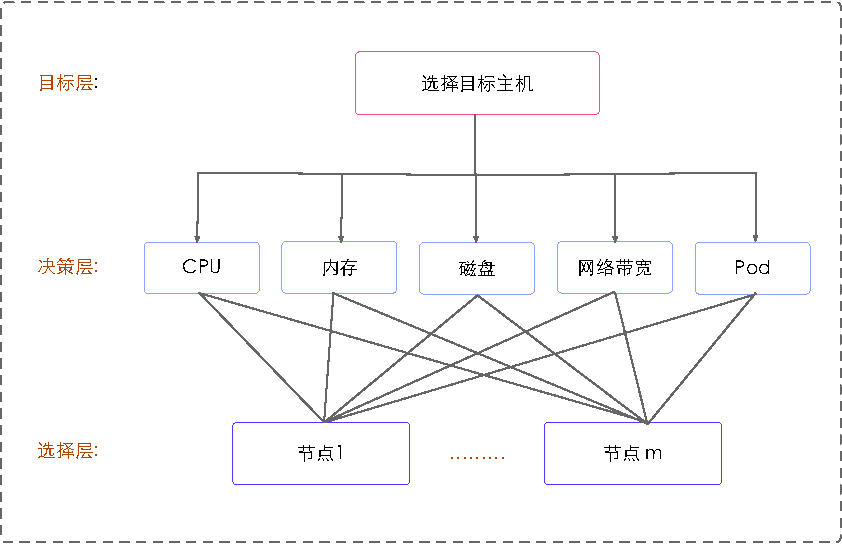
\includegraphics{fahp-model}
	\caption{多维资源递阶模糊层次结构}
\end{figure}
在云计算数据中心,CPU和内存一般是相对稀缺的资源,容器应用中CPU和内存相对其他资源需求重要性一般要高。单个节点上部署Pod数量较大,已部署Pod这个影响决策的因素相对其他因素的重要性较弱,但是大量小资源需求Pod会增加节点的管理成本。在构建模糊成对比矩阵时,该因素的模糊数较小,只是作为平衡各节点已部署Pod数量,容器应用的资源需求才是首要考虑因素。根据上述的层次结构图,下面介绍权重参数的自动求解方法。

\subsection{多维资源权重参数自动求解}
容器应用多维资源模糊层次结构如图4.3所示,大量容器应用进行模糊成对比矩阵构建时完全依赖人工判断既不准确也不适用于生产环境。在实际系统中,需要对每一个容器应用的多维资源进行权重参数求解,自动构建模糊成对比矩阵,然后转化为割集矩阵和判断矩阵,实现最大特征值的自动求解和判断矩阵的一致性检测。若判断矩阵不满足一致性要求,程序需要能自动调整判断矩阵直至其满足一致性检验。因此,如何对影响决策的CPU、内存、磁盘、网络带宽和已部署Pod等几个影响决策的因素构建模糊成对比矩阵成为解决问题的关键,整体的解决思路是用待调度容器资源需求占单位资源组的比例进行两两对比。设某个容器应用对各维度资源的需求和节点单位资源组如表4.3所示,需要求解容器应用各维度资源的权重系数$w_{c},w_{m},w_{d},w_{b},w_{p}$且$w_{c}+w_{m}+w_{d}+w_{b}+w_{p}=1$。
\begin{table}[htbp]
	\centering\dawu[1.3]
	\caption{某容器应用和节点单位资源组}
		\begin{tabular}{|p{1.5cm}<{\centering}|p{1.5cm}<{\centering}|p{1.5cm}<{\centering}|p{1.5cm}<{\centering}|p{1.8cm}<{\centering}|p{1.5cm}<{\centering}|} \hline
			Resources & CPU & Memory & Disk & Bandwidth & Pod \\ \hline
			U-Node & C & M & D & B & ..  \\ \hline
			Pod & $C_{0}$ & $M_{0}$ & $D_{0}$ & $B_{0}$ & 1  \\ \hline
			Weight & $w_{c}$ & $w_{m}$ & $w_{d}$ & $w_{b}$ & $w_{p}$ \\ \hline
		\end{tabular}
\end{table}

在构建模糊成对比矩阵时,根据容器应用资源需求和单位资源组的比值之间的差值确定模糊数。如在对比CPU和内存的重要性时,采用$|C_{0}/C-M_{0}/M|$作为判断依据,使用$\widetilde{1}\sim\widetilde{9}$表示相对重要程度的大小,在[0,1]范围内将其切分为5等份,根据比值差值自动构建模糊数。模糊成对比矩阵的模糊数、容器应用各维度资源需求和单位资源组的比值差值对应如表4.4所示。在数据中心的集群中,各节点的资源构成通常是异构的,即单个服务器各维度资源不同,不能直接使用容器应用与各节点资源比值的差值获取模糊数,需要抽象出单位资源组概念作为构建依据。如1个core的CPU、1G内存、50G磁盘、10M带宽作为一个单位资源组,单位资源组的大小根据集群实际情况确定,将容器应用和单位资源组的比值差值作为模糊数的依据。最后使用表4.4的方法构建模糊成对比矩阵。
\begin{table}[htbp]
	\centering\dawu[1.3]
	\caption{模糊数和资源比值差值对应表}
	\begin{tabular}{|p{1.8cm}<{\centering}|p{1.8cm}<{\centering}|p{1.8cm}<{\centering}|p{1.8cm}<{\centering}|p{1.8cm}<{\centering}|p{1.8cm}<{\centering}|} \hline
		差值 & (0, 0.2] & (0.2, 0.4] & (0.4, 0.6] & (0.6, 0.8] & (0.8, 1) \\ \hline
		模糊数 & $\widetilde{1}$ & $\widetilde{3}$ & $\widetilde{5}$ & $\widetilde{7}$  & $\widetilde{9}$  \\ \hline
		差值 & (-0.2,0] & (-0.4, -0.2] & (-0.6, -0.4] & (-0.8, -0.6] & (-1, -0.8]  \\ \hline
		模糊数 & $\widetilde{1}^{-1}$ & $\widetilde{3}^{-1}$ & $\widetilde{5}^{-1}$ & $\widetilde{7}^{-1}$ & $\widetilde{9}^{-1}$  \\ \hline
	\end{tabular}
\end{table}

针对已部署Pod这一影响调度的因素,其重要性相对其他资源要低,容器应用对该资源的需求以及节点上能部署的Pod总数都无法度量,不能像其他资源一样直接通过比值的差值作为模糊数的获取依据。因此,将CPU、内存、磁盘和网络带宽四种资源的比值从小到大排序,相较于Pod这一因素的重要性依次获得模糊数为(${\widetilde{3},\widetilde{5},\widetilde{7},\widetilde{9}}$),反之,Pod相对于其他资源的模糊数为(${\widetilde{3}^{-1},\widetilde{5}^{-1},\widetilde{7}^{-1},\widetilde{9}^{-1}}$)。

容器应用资源需求和单位资源组比值的差值可以获取各因素之间两两对比的模糊数,从而构建模糊成对比矩阵,最终自动获取割集矩阵和判断矩阵。求解出判断矩阵的特征值和对应的特征向量,判断矩阵满足一致性判断后,归一化出各因素的权重值,实现权重参数的自动求解。下面用一个实际的例子详细展示模糊成对比矩阵的构建以及最终权重参数的求解过程。

若某个集群的单位资源组配置如表4.5所示,集群中各节点各维度资源的配置都是单位资源组的整数倍,单位资源组是构成集群资源的最小组成单元。提出单位资源组的概念主要是为解决异构集群的场景,通常数据中心的集群都是异构的,尤其是在云计算中心中,需要将互联网上大量闲置的计算机作为服务计算单元,这种整合的闲置资源,并不是同构服务集群。
\begin{table}[htbp]
	\centering\dawu[1.3]
	\caption{物理集群单位资源组配置}
	\begin{tabular}{|p{2cm}<{\centering}|p{2cm}<{\centering}|p{2cm}<{\centering}|p{2cm}<{\centering}|p{2cm}<{\centering}|} \hline
		类型 & CPU(M) & MEM(M) & Disk(G) & BW(M) \\ \hline
		数量 & 1200 & 8000 & 500 & 50  \\ \hline
	\end{tabular}
\end{table}

在该数据中心集群上进行应用容器的调度,设某个应用容器对各维度资源的需求和集群单位资源组的比值如表4.6所示。
\begin{table}[htbp]
	\centering\dawu[1.3]
	\caption{某应用容器的资源需求}
	\begin{tabular}{|p{1.8cm}<{\centering}|p{1.8cm}<{\centering}|p{1.8cm}<{\centering}|p{1.8cm}<{\centering}|p{1.8cm}<{\centering}|p{1.8cm}<{\centering}|} \hline
		类型 & CPU(M) & MEM(M) & Disk(G) & BW(M) & Pod \\ \hline
		数量 & 300 & 1100 & 210 & 40 & 1 \\ \hline
		占比 & 0.25 & 0.1375 & 0.42 & 0.8 & - \\ \hline
	\end{tabular}
\end{table}

根据各维度资源所占比值的差值作为模糊数的依据,可以构建出该容器应用的模糊成对比矩阵,已部署Pod因素影响较弱,其他因素与该因素对比获取的模糊数较大。自动构建的模糊成对比矩阵如式(4-12)所示,行和列依次为CPU、内存、磁盘、网络带宽以及已部署Pod等影响决策的因素,通过两两对比确定模糊数后获得一个5*5的模糊成对比方阵。
\begin{equation}
\widetilde{A} = \left\{\begin{array}{ccccc}
1 & \widetilde{1} & \widetilde{1}^{-1} & \widetilde{5}^{-1} & \widetilde{5}  \\
\widetilde{1}^{-1} & 1 & \widetilde{3}^{-1} & \widetilde{7}^{-1} & \widetilde{3} \\
\widetilde{1} & \widetilde{3} & 1 & \widetilde{3}^{-1} & \widetilde{7} \\
\widetilde{5} & \widetilde{7} & \widetilde{3} & 1 & \widetilde{9} \\
\widetilde{5}^{-1} & \widetilde{3}^{-1} & \widetilde{7}^{-1} & \widetilde{9}^{-1} & 1 \\
\end{array}\right\}
\end{equation}

给定割集参数$\alpha=0.5$,优化参数$\mu=0.5$,参数$\alpha$反映模糊数中最大可能值的模糊程度,即真实值与最大可能值的距离,当$\alpha=1$时,模糊数的真实值就是最大可能值,$\alpha=0$时模糊程度出现最大范围,真实值和最大可能值接近程度最低。$\mu$作为优化参数,在模糊给定$\alpha$后反映上界和下界的取值,$\mu=1$时取上界值,$\mu=0$时取下界值。两个参数对权重参数的影响可以参考文献[26],该文献对两个参数对权重产生的影响进行了详细的分析。将上述的模糊成对比矩阵转化为割集矩阵,然后再转变为实际判断矩阵如(4-13)所示。
\begin{equation}
A = \left\{\begin{array}{ccccc}
1 & \frac{3}{2} & \frac{3}{4} & \frac{5}{24} & 5 \\
\frac{3}{4} & 1 & \frac{3}{8} & \frac{7}{48} & 3 \\
\frac{3}{2} & 3 & 1 & \frac{3}{8} & 7 \\
5 & 7 & 3 & 1 & 9 \\
\frac{5}{24} & \frac{3}{8} & \frac{7}{48} & \frac{9}{80} & 1 \\
\end{array}\right\}
\end{equation}

使用特征向量法求解判断矩阵的特征值和对应的特征向量,获得的特征值$\lambda_{max}=5.2498$,计算一般一致性指标CI=(5.2498-5)/4=0.0623,查找随机一致性RI表在n=5时其值RI=1.12,因此随机一致性比率CR=CI/RI=0.0558<0.1,判断矩阵满足随机一致性比率CR<0.1的要求。

满足一致性的判断矩阵A最大特征值$\lambda_{max}$对应的特征向量$\nu_{max}$的值为(0.2291, 0.1452, 0.3607, 0.8903, 0.0600),将该特征向量归一化获得容器应用CPU、内存、磁盘、网络带宽以及已部署Pod几个因素的权重系数$w=(w_{c}, w_{m}, w_{d}, w_{b}, w_{p})=(0.136, 0.086, 0.214, 0.528, 0.036)$。从权重参数可以看出,该容器应用是一个网络密集型的应用,该应用对网络带宽资源需求更多,其权重参数最大,因此,权重参数也能反映容器应用对某个维度资源的需求量。至此,一个完整的自动构建模糊成对比矩阵并实现各维资源权重参数自动求解过程完成。

MRWS调度算法中,容器应用在进行调度时需要对集群中节点进行评分,选择评分最高的节点作为容器调度目标,在对节点空闲资源评分时需要使用容器应用需求资源权重系数作为乘积系数。在式(3-4)和(3-8)中,$\alpha$系数就是待调度容器应用各维资源的权重系数,该系数大小反映待调度容器对某个维度资源需求量。如一个CPU密集型应用,系数$\alpha_{1}$较大,节点中若某个节点CPU资源空闲较多,则该节点评分相对较高,Pod调度到该节点的几率就越大。使用FAHP对待调度容器Pod各维资源进行层次建模后,通过容器应用资源需求和集群单位资源组比值之间的差值构建模糊成对比矩阵,最终自动求解的各维资源权重值就是空闲资源评分系数。其中单位资源组大小、$\alpha$割集系数和优化参数$\mu$的选取对调度评分都至关重要。使用系数调节后的MRWS算法可以实现容器云集群中各维资源的均衡利用,将CPU密集型应用调度到CPU剩余资源较多并且各维资源使用较为平衡的节点上,其他密集型的应用调度相似。因此,这种调度方法将各种密集型容器应用尽可能分散混合部署到节点上,避免大量相同密集型集中调度到相同节点上,造成某一维度的资源资源不足,尤其是在大数据处理多维计算框架应用调度的场景下,能够提升集群资源利用率和负载均衡性,极大增强集群的服务性能。

\section{本章小结}
在MRWS调度算法设计中,需要求解容器应用各维度资源的权重参数作为节点评分乘积系数,本章应用FAHP求解容器应用各维资源权重参数。首先从层次分析法AHP开始,详细介绍该方法的历史背景和解决问题的能力。为减少专家判断的主观性和模糊性,使用各种分布函数作为模糊数,选定三角模糊数作为判断依据,从而引入了模糊层次分析法FAHP,并使用$\widetilde{1}\sim\widetilde{9}$表示因素之间相对重要程度。接着详细阐述应用该方法求解权重系数的步骤,构建模糊成对比矩阵,给定置信度$\alpha$将其转化为割集矩阵,设置优化参数$\mu$后转化为判断矩阵,求解判断矩阵最大特征值和特征向量,检测该判断矩阵是否满足一致性要求。通过调整判断矩阵,满足一致性判断要求后,归一化最大特征值对应的特征向量获得各维度资源的权重值,接着通过一个力学系数的例子展示各计算步骤的详细计算过程。

最后,使用FAHP求解容器应用各维度资源的权重参数,先对各资源需求和备选节点进行层次建模,获得一个全层次的模型结构。将容器应用各维度资源和单位资源组的比值之间的差值作为自动构建模糊成对比矩阵的依据,获得模糊成对比矩阵,并转化为割集矩阵和判断矩阵,实现权重参数的自动求解。使用一个具体的容器应用展示该应用各维度资源的权重系数自动计算过程,最终获得的权重参数就是MRWS调度算法中用于各节点空闲资源和资源平衡性的评分乘积系数。









\chapter{OpenShift容器云平台和MRWS实验}
提出MRWS调度方案优化OpenShift容器云平台底层容器编排引擎Kubernetes调度流程和调度算法后,需要对其资源利用率和负载均衡性进行评估测试。本章主要实验包括如下几个部分:
\begin{enumerate}[(1)]
	\item 在ContainerCloudSim容器云仿真平台上进行大规模容器应用仿真调度实验、对比Kubernetes默认算法、Random算法和MRWS调度算法在资源利用率和负载均衡性方面的性能。
	\item 基于开源OpenShift Origin搭建开发了Paladin容器云平台,该平台是一个集海量数据存储管理、多计算框架快速部署、调度优化、用户注册、按需服务等多功能的容器云PaaS平台。
	\item 在Paladin开发多种分布式计算框架,将其打包成镜像文件,存储在镜像仓库汇中,用户可以快速构建开发测试环境。
	\item 在Paladin平台上开发MRWS算法的调度器,使用多中计算框架容器应用混合部署测试其性能,并与其他调度算法进行对比。
\end{enumerate}

\section{ContainerCloudSim模拟MRWS调度方案}
实验室基于开源OpenShift Origin开发的容器云PaaS平台是在小规模实际物理机上部署,不能进行调度方案的大规模测试和分析,为了评估方案的性能和可靠性,首先在容器云仿真平台ContainerCloudSim上进行大规模的仿真实验。首先构建仿真实验环境,然后开发Kubernetes默认Default调度算法、Random和MRWS调度算法,使用大规模负载进行测试分析。

\subsection{ContainerCloudSim容器云仿真平台}
\subsubsection{CloudSim云仿真平台}
容器和容器编排技术的逐渐成熟推动了容器云的飞速发展,在计算中心的容器云上为了评测资源调度策略和容器服务性能,一个容器云仿真平台变得异常重要。经过大量测试对比调度方案,不仅可以节约开发时间,也能避免造成资源浪费和减少试错成本。针对每一个调度方案,如果部署大规模容器云平台进行性能分析测试,绝大多数的小公司和开发人员并不具备这种条件。在传统的云计算模式下,应用服务的组成、供应、配置和部署条件较为复杂,当用户需求和系统配置动态变化时,评估一个调度策略以及工作负载是相当困难的,一个优秀的云计算平台模拟器可以很好解决这个问题。一个云平台模拟器通过控制环境变量和重复试验可以加速理论研究和开发过程,根据需求和应用场景不同,各大公司和研究机构推出了一系列的云计算平台仿真工具。

MDCSim是一个全面、灵活、可扩展的多层数据中心模拟器,整个模拟平台分为通信层、内核层和用户层建模,通信层用于模拟模拟集群内部通信、内核层模拟调度和分析系统性能、用户层用于模拟各种应用。该模拟器可以根据底层不同硬件特点进行混合建模,用于评估数据中心的能耗,让用户在保持低功耗的同时实现集群服务性能的提升。GroudSim是一个基于Java的模拟器,用于模拟科学应用在网格和云设施上执行问题,模拟完成后给用户提供了基础的统计和分析功能。NetworkCloudSim用于解决网络模拟问题,弥补其他模拟器对网络细节关注不足,支持MPI和工作流。TeachCloud用于对MapReduce应用建模并集成一个负载生成器,提供图形化的接口和实现定制的网络拓扑结构。CloudSim是墨尔本大学Gridbus项目推出的云计算仿真软件,既能对系统性能和应用服务模拟、仿真、试验,也能评估资源调度策略的优劣。

CloudSim是一个开源的仿真软件,最大特点就是提供一个虚拟化引擎,帮助数据中心建立和管理各种虚拟化服务。支持大规模云计算资源管理和调度模拟,将数据中心的资源虚拟化为资源池,CloudSim的分层体系架构图如5.1所示。
\begin{figure}[H] % use float package if you want it here
	\centering
	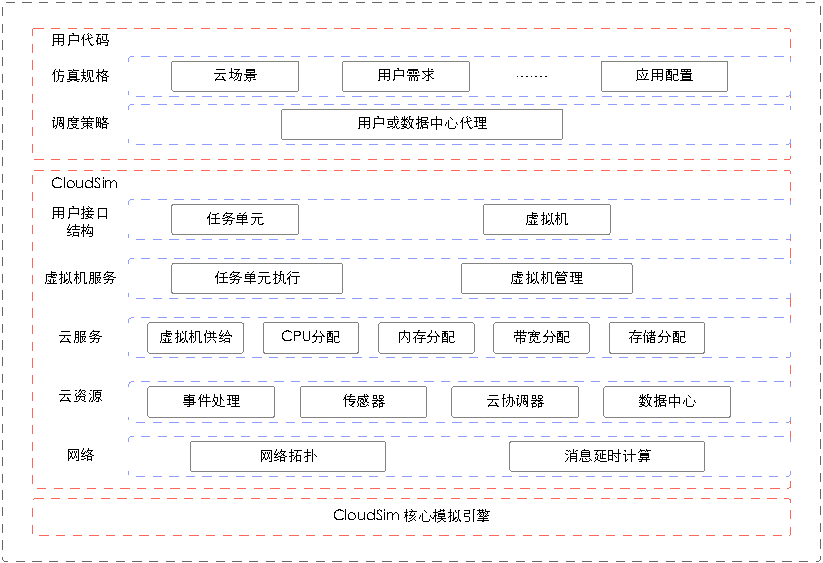
\includegraphics{cloudsim-layer}
	\caption{CloudSim分层架构图}
	\label{fig:xfig1}
\end{figure}

CloudSim是一个分层构建的体系结构,从下到上一次为CloudSim核心引擎层、网络、云资源、云服务、虚拟服务、用户接口结构、资源调度以及仿真规格层。下面一次介绍各层次的大致作用:
\begin{enumerate}[(1).]
	\item CloudSim核心引擎层是离散数据模拟引擎SimJava,为上层提供系统组件构建如服务、数据中心、客户端、代理、虚拟机等,查询和时间处理、通信、模拟时钟等功能。
	\item Network层模拟网络组件如资源收集、数据集、负载测试、信息服务等,对网络设施建模,支持高层软件组件。
	\item 云资源层主要是Host主机和数据中心,主机的核心硬件设施通过数据中心类建模,处理服务请求,构成虚拟资源池。
	\item 云服务层给客户端分配特定应用的VM,同时给VM分配处理内核、内存、磁盘以及网络带宽,可以执行用户新的VM提供策略,有助于一定目标优化。
	\item 虚拟机服务层提供任务执行和虚拟机管理,定义一系列虚拟机创建、销毁、合并、迁移等操作管理,执行基于云环境的应用服务。
	\item 用户接口层向用户提供VM任务单元和虚拟机,将下层的虚拟资源打包成虚拟机提供给用户。
	\item 用户代码层是用户根据实际应用场景和需求,定制应用的规格和调度策略,将应用加入数据中心的代理中,按照资源调度策略进行调度。
\end{enumerate}
CloudSim有一些重要的类和核心概念,针对这些类的大致作用进行简单的介绍:
\begin{enumerate}[1.]
	\item DataCenter类封装底层的Host主机,提供虚拟化的资源,保证每个数据中心至少存在一台运行的Host主机,同时提供虚拟化网络并内置了一个调度组件,为虚拟机和主机分配CPU、内存、网络带宽等资源。
	\item DataCenterBroker类是数据中心代理,负责虚拟机和云任务列表的提交。
	\item VM类是虚拟机类,运行在Host上,多个VM共享Host资源。
	\item Cloudlet类是云任务类,根据用户的设置构建云计算和调度任务。
	\item VmAllocationPolicy类是虚拟机分配策略类,该类实现了虚拟机分配给Host主机的调度策略,用户可以重写该分配策略。
	\item CloudletScheduler类实现多种分配策略,虚拟机内部应用共享处理器的策略,时间共享还是空间共享。
\end{enumerate}

此外,CLoudSim还有数据中心资源配置类DataCenterCharacteristics、扩展虚拟机分配策略的主机类Host、带宽分配策略类BwProvisioner、模拟网络延时行为类NetworkTopology、模拟存储区域网类SanStorage、虚拟分配主存类RamProvisioner、云协调器类CloudCoordinator等一些列重要的类,共同完成CloudSim功能。

\subsubsection{ContaienrCloudSim容器云仿真平台}
随着容器技术的迅猛发展,CaaS(Congtianer as a Service)作为一种新型的服务模式变得越来越普遍。上述介绍的各种云计算仿真平台以及早期的CloudSim版本并不支持容器仿真,一个支持容器应用仿真的平台变得越加紧迫。为了缩短容器云上新方法的开发时间,墨尔本大学的研究人员利用CloudSim虚拟化的特点,在其基础上开发了ContainerCloudSim,专门用于数据中心容器应用的模拟。在最新的CloudSim-4.0上已经集成ContainerCloudSim,提供Docker容器应用仿真支持,ContainerCloudSim与CloudSim生态圈关系如图5.2所示。
\begin{figure}[H] % use float package if you want it here
	\centering
	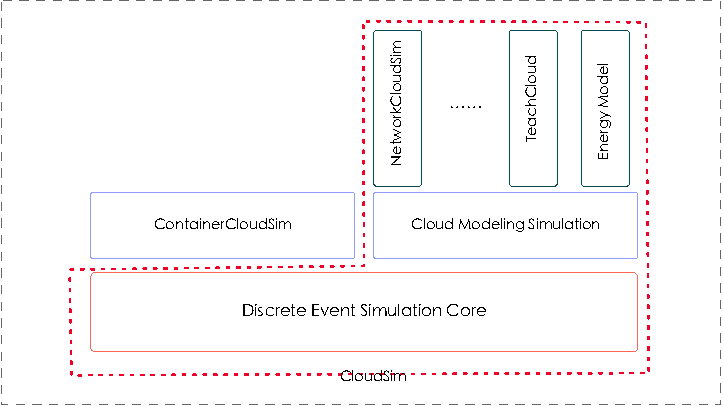
\includegraphics{container-cloudsim}
	\caption{ContainerCloudSim与CloudSim生态圈}
\end{figure}
集成ContainerCloudSim的CloudSim-4.0云平台模拟器已完整支持容器云的仿真,新的版本具有如下几个特点:
\begin{enumerate}[(1)]
	\item 支持数据中心大规模云计算建模和仿真。
	\item 支持服务器虚拟化和主机的建模仿真,定制虚拟机调度策略。
	\item 支持容器应用程序的建模和仿真。
	\item 支持能量感知的计算资源建模和仿真。
	\item 支持网络拓扑结构和消息传递应用建模和仿真。
	\item 支持动态插入元素、停止和恢复的模拟。
	\item 支持混合云的建模和仿真。
\end{enumerate}

在ContainerCloudSim部分,提供容器、VMs、Host、数据中心资源包括CPU、内存和存储的管理功能,实现动态监控系统性、控制容器内应用的执行以及给容器提供虚拟机。容器的模拟器要能给研究人员提供容器调度方案间的对比,容器调度策略决定容器如何被调度到虚拟机上,以及各种调度算法之间的对比和评测。算法的能耗问题也是容器模拟器应该关注的重点,可以提供各种算法的能耗度量,容器的合并和迁移也是模拟器的一大功能。最后,模拟器要能够支持容器的扩展性,在CaaS容器环境中,容器的数量是远远多于虚拟机的。ContainerCloudSim是在CloudSim基础上开发而来,也是一个分层的架构,整体架构如下所示。
\begin{figure}[H] % use float package if you want it here
	\centering
	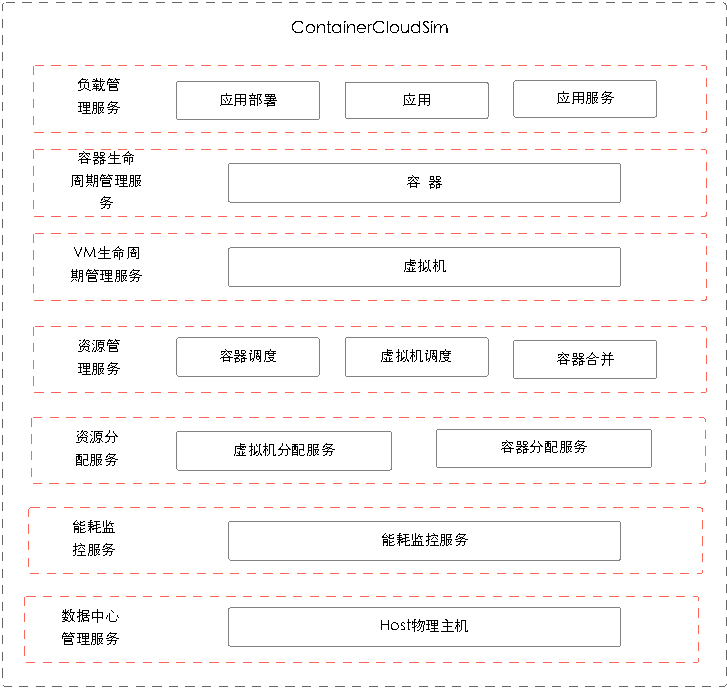
\includegraphics{containercloudsim-layer}
	\caption{ContainerCloudSim分层架构图}
\end{figure}
从底至上依次分为数据中心管理服务、能耗监控服务、资源分配服务、资源管理服务、虚拟机生命周期管理服务、容器生命周期管理服务和负载管理服务等。每个层次的大致作用如下:
\begin{enumerate}
	\item 负载管理服务层关注于客户端应用的注册、部署、调度、应用层级的性能以及应用健康监控。
	\item 容器生命周期服务管理层负责容器生命周期管理,包括创建容器、注册容器到系统中、启动、停止、重启、从一个主机迁移到另一个主机以及容器销毁。除此之外,还负责执行和管理在容器中任务,监控任务资源利用率。
	\item 虚拟机生命周期管理服务层负责虚拟机的管理包括创建、启动、停止、重启、销毁、迁移以及资源利用率监控。
	\item 资源管理服务层负责容器在满足资源需求和软件环境的虚拟机上创建,虚拟机在满足资源需求的主机上创建,由容器调度、虚拟机调度和合并服务构成。容器调度根据容器调度策略调度容器到虚拟机、虚拟机调度根据虚拟机调度策略调度虚拟机到主机,合并策略通过合并容器减少主机需求,最小化资源碎片。
	\item 资源分配层服务管理虚拟机和容器的资源分配,由容器分配服务和虚拟机分配服务构成。容器分配服务负责虚拟机资源分配给容器,虚拟机分配服务负责主机资源分配给虚拟机。
	\item 能耗监控服务负责数据中心主机能耗监控,构建必要的能耗模型。
	\item 数据中心管理服务负责管理数据中心资源,主机开关机以及监控资源利用率。
\end{enumerate}
至此,ContainerCloudSim容器云仿真平台介绍完毕,具体的仿真执行流程具体的实现可以参见其源代码。

\subsection{MRWS资源利用率实验}
在ContainerCloudSim容器云仿真平台上的ContainerPlacementPolicy库下开发MRWS、Kubernetes默认Default算法,该类自带Ramdom算法,对比三种算法下集群资源的利用率。该容器云仿真平台影响调度因素较多,需要根据实际的需要进行一些必要的设置。

首先MRWS算法和Kubernetes的Default算法在预选阶段使用的筛选规则相同,评分阶段除空闲资源评分函数和平衡函数外,其他评分函数相同。因此,假设其他评分函数和外部条件都相同的情况下,只需模拟比较MRWS算法和Default算发的空闲资源评分函数。在模拟器设置方面,要对比容器各种调度算法下集群资源的利用率和负载均衡性,对虚拟机的调度策略已有众多的研究,不是本文的研究方向,因此,假设ContainerCloudSim数据中心的单个Host上只运行一个虚拟机,且虚拟机的资源配置和Host主机相同。本文也不对Container的迁移算法做研究,需要在模拟器上设置容器禁止迁移,即不触发迁移阈值。由于只对容器应用调度研究,不执行具体的云任务,不设置容器、虚拟机和主机的PE数。测试负载是基于PlanetLab负载进行的更改,让CPU、内存、磁盘和带宽的利用率从10\%到90\%的随机变化。虚拟机、主机的配置如表5.1所以,CPU的单位是Mips,容器应用根据负载情况随机构建。在云数据中心中,集群通常是异构的,节点拥有资源数量不同,假设存在三种主机,用于模拟异构集群。
\begin{table}[H]
	\centering\dawu[1.3]
	\caption{主机和虚拟机配置表}
	\begin{tabular}{|p{1.8cm}<{\centering}|p{1.5cm}<{\centering}|p{2cm}<{\centering}|p{1.5cm}<{\centering}|p{1.5cm}<{\centering}|p{1.5cm}<{\centering}|p{1.5cm}<{\centering}|p{1.5cm}<{\centering}|} \hline
		Host类型 & VM类型 & CPU型号 & MIPS & 内存(G) & 磁盘(G) & 带宽(M) \\ \hline
		\#1 & \#1 & i7 7500U & 49360 & 16 & 1000  & 100 \\ \hline
		\#2 & \#2 & i5 8200U & 65770 & 32 & 1000 & 100 \\ \hline
		\#3 & \#3 & X6 1100T & 78440 & 16 & 1000 & 100 \\ \hline
	\end{tabular}
\end{table}

容器应用的配置根据模拟的负载情况自动生成,并对生成的负载自动求解权重参数,参数设置部分代码片段如下:
\begin{lstlisting}[ language=Java]
public static final int VM_TYPES = 3;
public static final double[] VM_MIPS = new double[]{49360, 65770, 78440};
public static final int[] VM_PES = new int[]{};
public static final float[] VM_RAM = new float[] {(float)16000, (float) 32000, (float) 16000};//**MB*
public static final int VM_BW = 100;
public static final int VM_SIZE = 1000000;

public static final int HOST_TYPES = 3;
public static final int[] HOST_MIPS = new int[]{49360, 65770, 78440};
public static final int[] HOST_PES = new int[]{};
public static final int[] HOST_RAM = new int[]{1600,3200,1600};
public static final int HOST_BW = 100;
public static final int HOST_STORAGE = 1000000;

public static final int NUMBER_HOSTS = 30;
public static final int NUMBER_VMS = 30;
public static final int NUMBER_CLOUDLETS = 200;
\end{lstlisting}

模拟实验中设置资源阈值为0.15,一旦节点上的某种资源使用率超过该阈值后将不能部署新的容器应用,模拟实验主要测量在相同数量容器下需要服务器的数量。若节点资源利用越均衡,该节点可部署的容器应用数量越多,从而需要的节点数量越少。实验对比MRWS调度算法、Kubernetes的Default算法简称为KUB算法、Random算法以及FirstFit算法对资源的需求,后两种算法是ContainerCloudSim自带算法,只需要模拟KUB的内存和CPU均衡利用,MRWS综合考虑CPU、内存、磁盘、网络带宽以及已部署Pod应用因素的综合评分算法。模拟实验中单位资源组$res=(cpu,memory,disk,bandwidth)=(10000Mips,4000M,100G,10M)$,单个应用容器的负载是单位资源组的$10\%\sim 90\%$随机变化的资源需求,构建出的应用容器负载如表5.2所示。
\begin{table}[H]
	\centering\dawu[1.3]
	\caption{N个应用容器的资源配置}
	\begin{tabular}{|p{1.8cm}<{\centering}|p{1.8cm}<{\centering}|p{1.8cm}<{\centering}|p{1.8cm}<{\centering}|p{1.8cm}<{\centering}|p{1.8cm}<{\centering}|} \hline
		应用容器 & CPU(MIPS) & 内存(M) & 磁盘(G) & 带宽(M) & Pod \\ \hline
		 1 & 8500 & 680 & 34 & 9 &1 \\ \hline
		 2 & 4000 & 840 & 12 & 16 & 1 \\ \hline
		 3 & 2000 & 3400 & 20 & 6 & 1 \\ \hline
		 4 & 3400 & 1200 & 80 & 10 & 1 \\ \hline
		 ... & ... & ... & ... & ... & ... \\ \hline
		 N & 7600 & 600 & 30 & 4 & 1 \\ \hline
	\end{tabular}
\end{table}
根据MRWS的FAHP自动建模和按照资源需求比值的差值构建模糊成对比矩阵,自动求解容器应用各维度资源的权重参数,上述容器列表各维度资源对应的权重参数如表5.3所示。
\begin{table}[H]
	\centering\dawu[1.3]
	\caption{应用容器资源对应的权重参数表}
	\begin{tabular}{|p{1.8cm}<{\centering}|p{1.8cm}<{\centering}|p{1.8cm}<{\centering}|p{1.8cm}<{\centering}|p{1.8cm}<{\centering}|p{1.8cm}<{\centering}|} \hline
		应用容器 & CPU(MIPS) & 内存(M) & 磁盘(G) & 带宽(M) & Pod \\ \hline
		 1 & 0.528 & 0.086 & 0.136 & 0.214 & 0.036 \\ \hline
		 2 & 0.185 & 0.128 & 0.082 & 0.570 & 0.035 \\ \hline
		 3 & 0.092 & 0.596 & 0.119 & 0.158 & 0.035 \\ \hline
		 4 & 0.140 & 0.095 & 0.508 & 0.221 & 0.036 \\ \hline
		 ... & ... & ... & ... & ... & ... \\ \hline
		 N & 0.596 & 0.092 & 0.158 & 0.119 & 0.035 \\ \hline
	\end{tabular}
\end{table}
测试在相同容器应用数量的条件下所需虚拟机的数量,根据前面一个主机Host上只运行一个和主机配置相同虚拟机,因此虚拟机的数量也是Host主机的数量。实验开始时给定一定数量的Host,三种类型Host数量相同,一旦出现所有主机都无法满足新的容器资源需求,同时增加三种类型Host一台。如200个应用容器时先给定18台主机,以后每次各类型增加一台,即每次增加三台主机,避免某一类型的主机数量过多,测试结果如表5.4所示。
\begin{table}[H]
	\centering\dawu[1.3]
	\caption{相同容器数量下各算法所需主机数}
	\begin{tabular}{|p{1.8cm}<{\centering}|p{1.5cm}<{\centering}|p{1.5cm}<{\centering}|p{1.5cm}<{\centering}|p{1.5cm}<{\centering}|p{1.5cm}<{\centering}|p{1.5cm}<{\centering}|} \hline
		\diagbox[innerwidth=1.8cm]{算法}{容器数} & 200 & 400 & 600 & 800 & 1000 & 1200 \\ \hline
		MRWS & 21 & 42 & 60 & 78 & 96 & 114 \\ \hline
		KUB & 21 & 45 & 69 & 87 & 105 & 129 \\ \hline
		Random & 24 & 48 & 72 & 93 & 117 & 139 \\ \hline
		FirstFit & 27 & 54 & 81 & 108 & 138 & 162 \\ \hline
	\end{tabular}
\end{table}
从上表5.4可以得出,在应用容器数量集群规模较小的情况下,各种算法对主机数量需求相差不大,MRWS调度算法的优势并不明显。这是由于集群中节点各维度资源过载现象较少,整体集群的资源利用率不也高。随着容器数量和主机数量的增加,Random和FirstFit算法劣势越加明显,相同数量下所需的主机数量更多,这是由于随机调度和首个合适节点调度方法容易造成大量相同密集型的应用部署到同一个节点,从而使某一维度资源过载,不能部署更多的应用。Kubernetes的Default算法考虑了CPU和内存的均衡性,其效果比其他两种算法要好,MRWS调度算法综合考虑了各维度资源的均衡性,其效果最佳,所需主机数量最少。MRWS还考虑节点已部署Pod因素,在资源利用率相差不大的情况下避免某个节点部署大量较小资源需求的容器应用,给节点容器管理造成过大开销,从而降低集群性能。容器应用应该分散和均衡地部署到集群的各节点上,提升集群服务性能。

\subsection{MRWS负载均衡实验}
集群服务性能一个关键问题就是负载均衡,而调度策略是影响负载均衡的核心因素。好的负载均衡策略不仅可以提升集群负载处理能力,缩短任务执行时间,也能有效避免单点故障。当前服务器的负载均衡算法一般有随机算法、轮询和加权轮询、最小连接和加权最小连接、哈希算法、IP散列法以及URL散列等。一些重用的负载均衡组件有Apache、Nginx、LVS(Linux Virtual Server)、HAproxy、KeepAlived、Memcached等。Apache和Nginx是一个HTTP的服务器,具有反向代理能力,通过对用户请求分流实现负载均衡;LVS是一个虚拟的服务器集群系统,可以实现Linux平台下简单的负载均衡;HAproxy提供高可用、负载均衡以及基于TCP和HTTP代理,适用于负载较大的web服务站点;KeepAlived也是一个组件,用于检测服务集群中故障节点,及时处理不健康的节点;Memcached是内存缓存系统,对于业务查询数据进行缓存,降低节点的负载,也是一个负载均衡组件。本文主要研究集群中各节点多维资源负载情况,目的在于新的调度方法是否具有更好的资源负载,各维度资源利用是否更加均衡。实验将从三个方面进行对比MRWS算法、Kubernetes的Default算法、Random算法和FirstFit算法中单个节点的相同维度资源、单个节点各维度资源均值、整个集群负载均衡性进行对比,评价指标如式(3-10、3-11)所示。测试过程中假定集群数量、应用容器数量不同的条件下上述三个指标的负载不均衡度。

首先测试集群中各节点某个维度资源利用均衡情况,希望集群中节点上某个维度资源如CPU利用率更加平滑,若节点上该维度资源波动过大则表明其服务性能可能会降低,下面以CPU为例,其他维度资源类似。
\begin{figure}[h]
	\centering%
	\begin{subfigure}{7cm}
		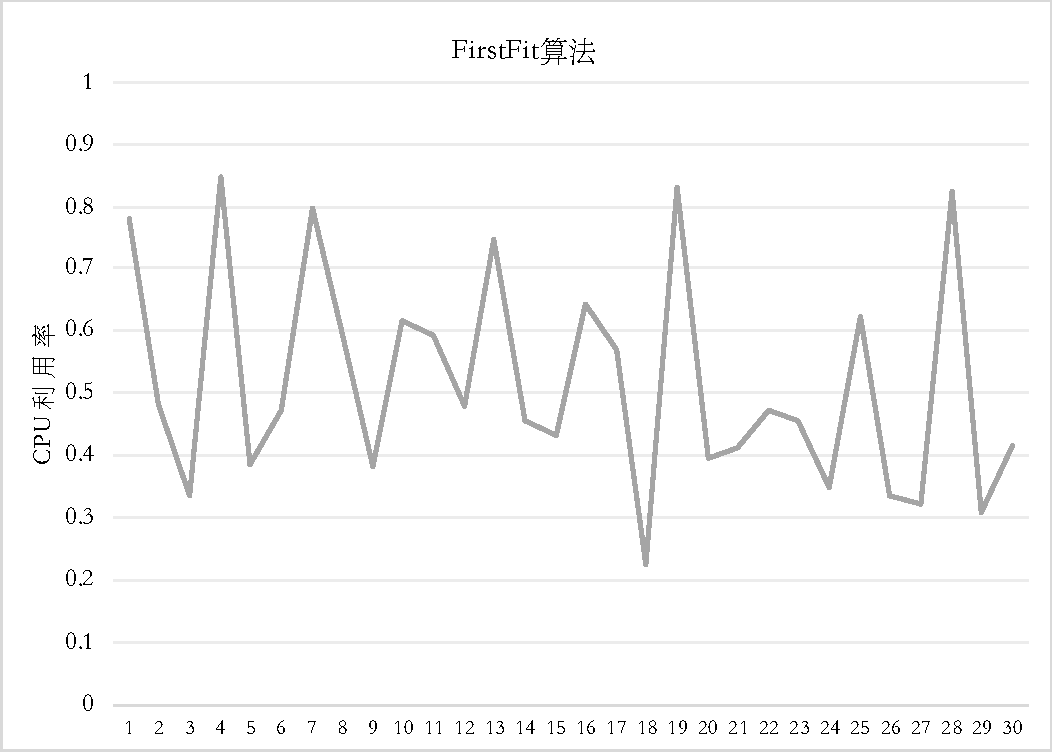
\includegraphics[width=7cm,height=5cm]{firstfit-cpu}
		\caption{FirstFit算法CPU利用率}
	\end{subfigure}%
	\hspace{0.5cm}%
	\begin{subfigure}{7cm}
		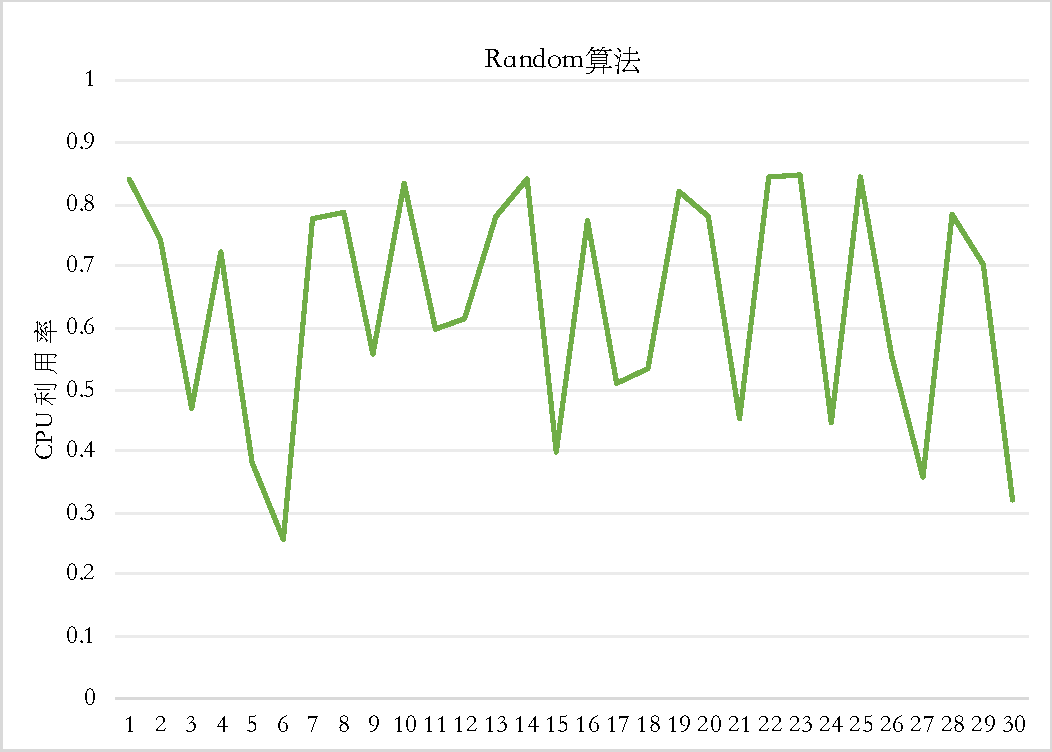
\includegraphics[width=7cm, height=5cm]{random-cpu}
		\centering{\caption{Random算法CPU利用率}}
	\end{subfigure}
	\begin{subfigure}{7cm}
		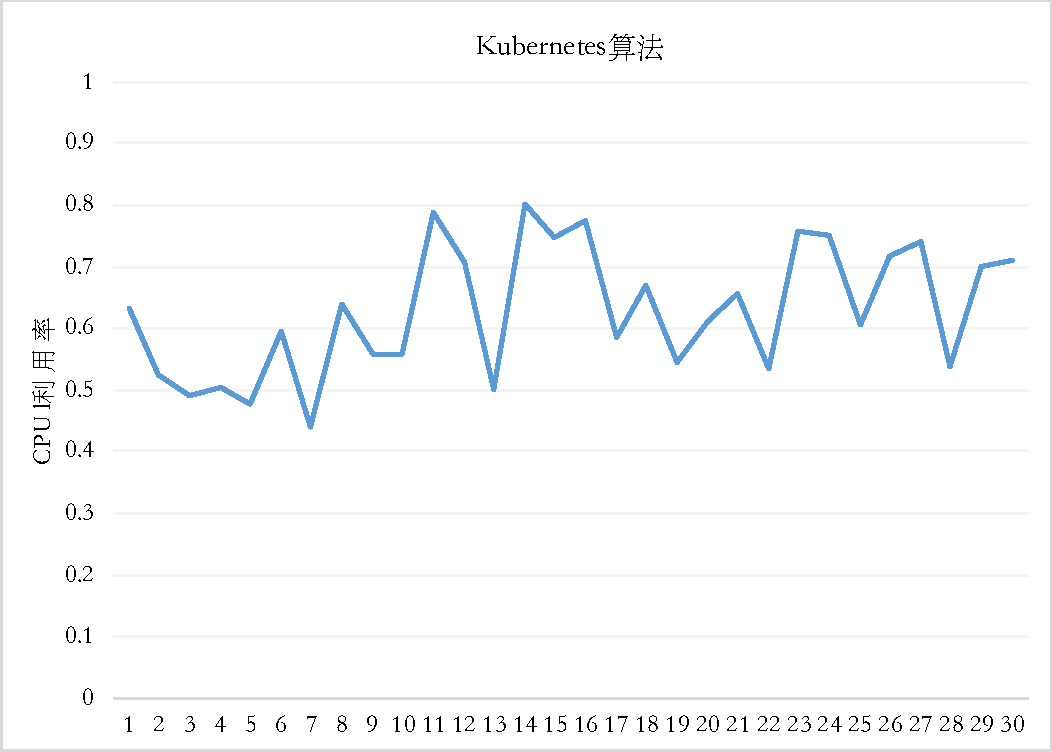
\includegraphics[width=7cm,height=5cm]{kub-cpu}
		\caption{kubernetes算法CPU利用率}
	\end{subfigure}%
	\hspace{0.5cm}%
	\begin{subfigure}{7cm}
		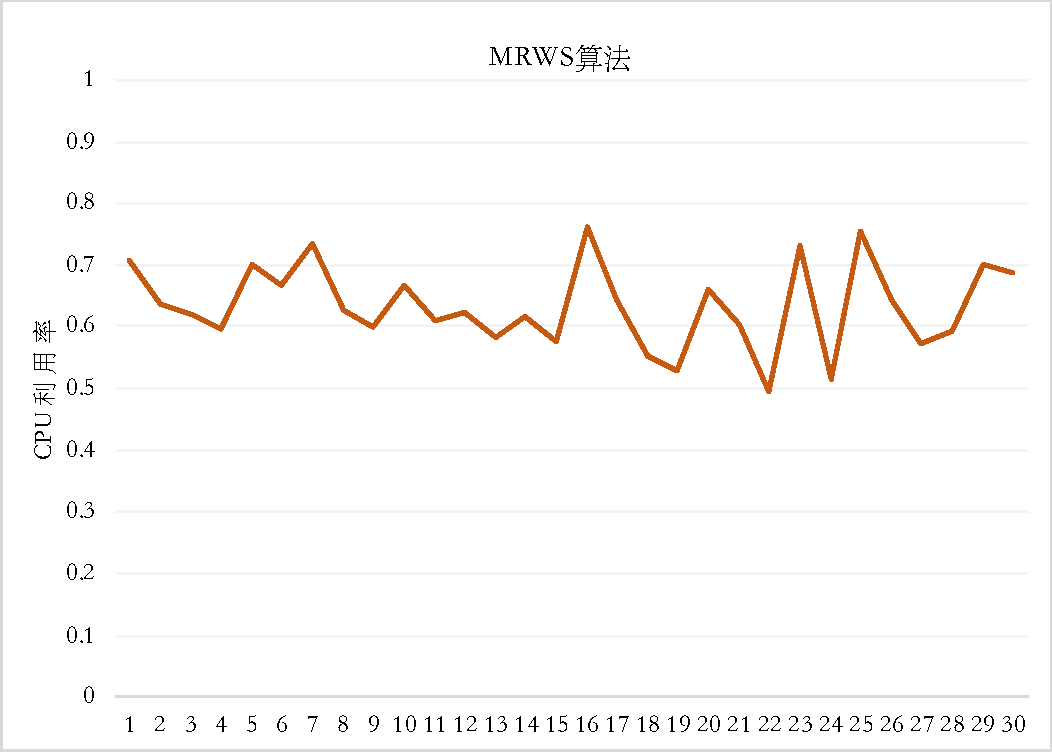
\includegraphics[width=7cm, height=5cm]{mrws-cpu}
		\centering{\caption{MRWS算法CPU利用率}}
	\end{subfigure}
	\caption{四种调度算法下节点CPU利用率波动图}
	
\end{figure}

从图5.4看出,MRWS调度算法下CPU利用率波动性较小,Kubernetes调度算法次之,Random和FirstFit算法节点CPU利用率波动较大。这是由于前两种算法都考虑了CPU利用的均衡性,其中Kubernetes在进行节点评分时考虑了CPU和内存平衡利用,MRWS调度算法综合考虑了CPU、内存、磁盘、网络带宽和已部署的Pod的因素。有效避免单个节点某个维度资源资源利用过高,出现过载现象,从而不能调度更多的应用,造成其他维度的资源浪费,MRWS算法能够有效提升集群的服务性能和资源利用率。下面的实验使用之前定义的均衡度对集群中单个节点上资源均衡度进行测量,实验中假设应用容器数量相同,分别用四种算法对其进行调度,计算单个节点的负载均衡度,部分节点的负载均衡度如下。

\begin{figure}[H]
	\centering%
	\begin{subfigure}{7cm}
		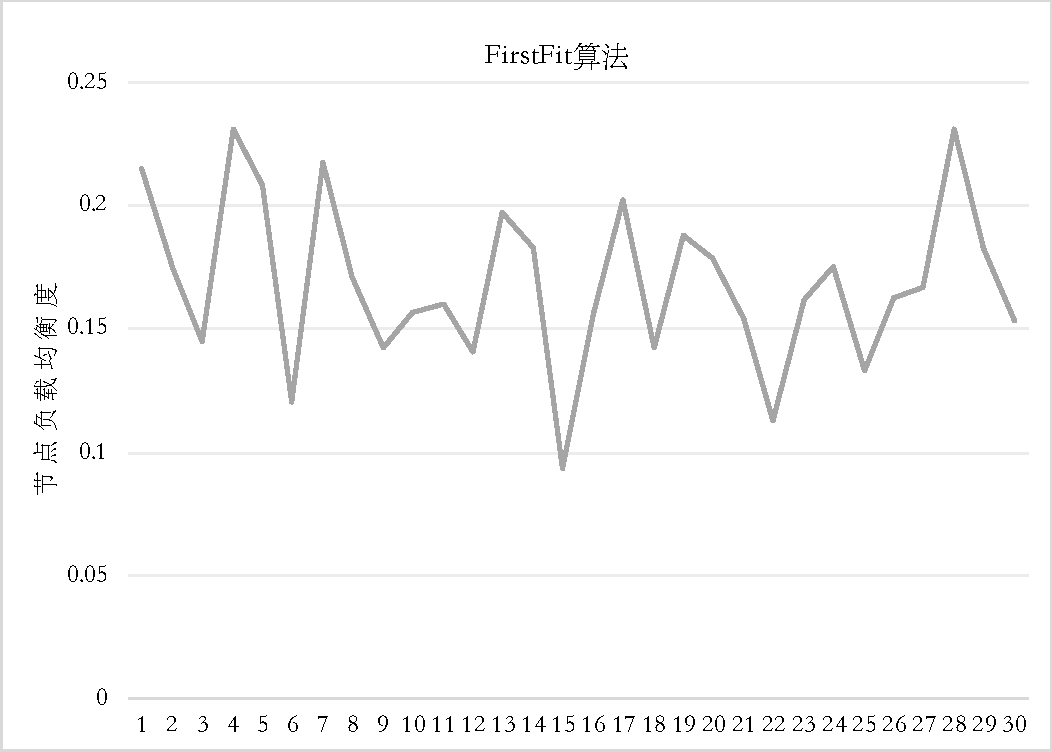
\includegraphics[width=7cm,height=5cm]{firstfit-ba}
		\caption{FirstFit算法节点负载均衡度}
	\end{subfigure}%
	\hspace{0.5cm}%
	\begin{subfigure}{7cm}
		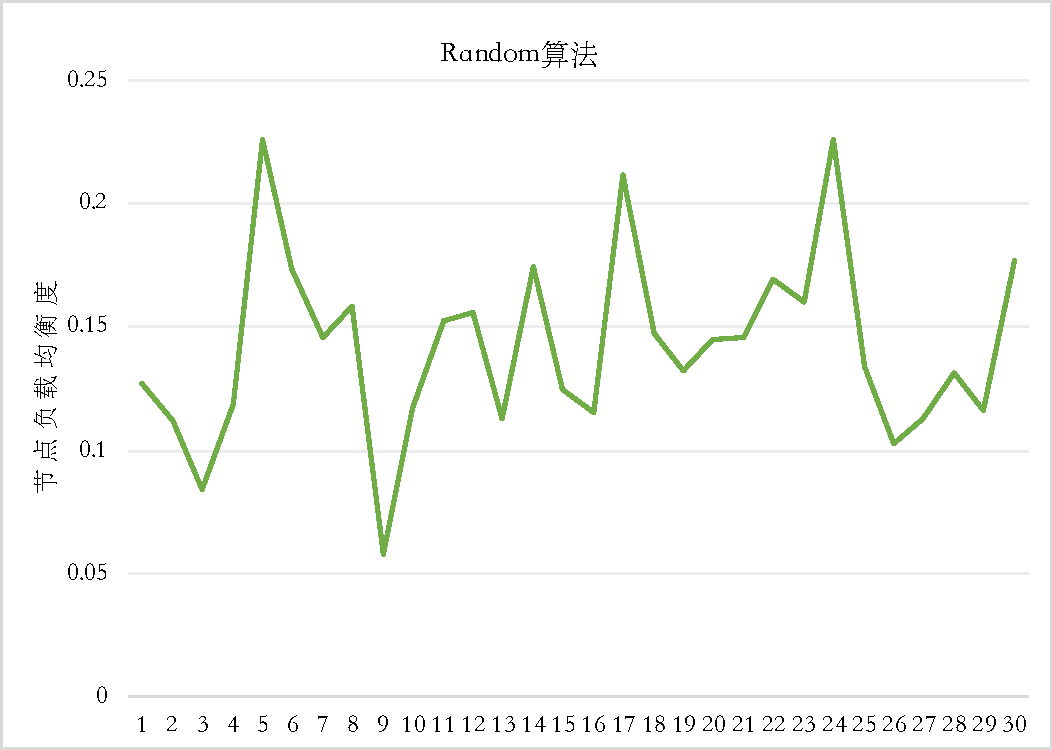
\includegraphics[width=7cm, height=5cm]{random-ba}
		\centering{\caption{Random算法节点负载均衡度}}
	\end{subfigure}
	\begin{subfigure}{7cm}
		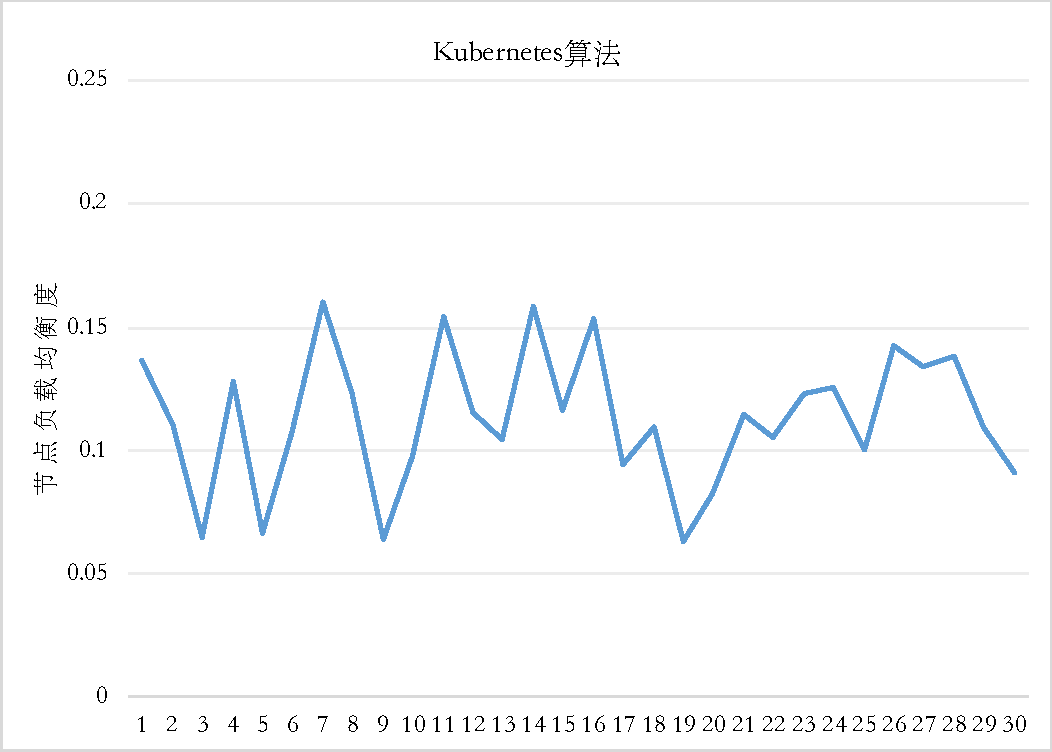
\includegraphics[width=7cm,height=5cm]{kub-ba}
		\caption{kubernetes节点负载均衡度}
	\end{subfigure}%
	\hspace{0.5cm}%
	\begin{subfigure}{7cm}
		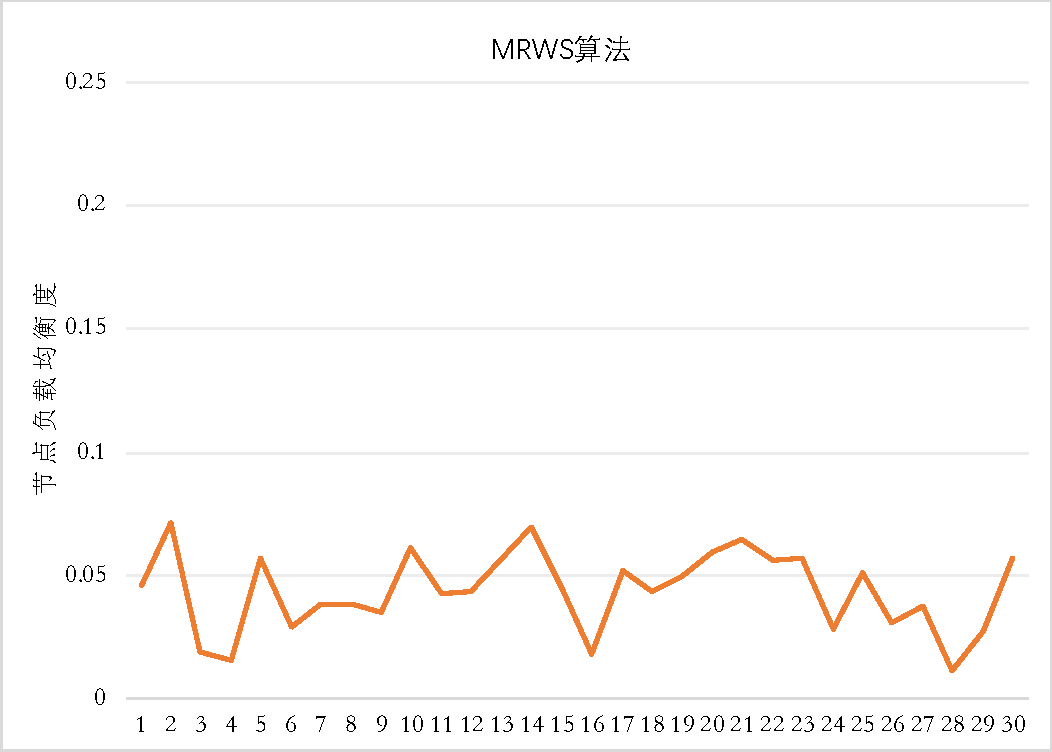
\includegraphics[width=7cm, height=5cm]{mrws-ba}
		\centering{\caption{MRWS算法节点负载均衡度}}
	\end{subfigure}
	\caption{四种调度算法下节点负载均衡度}
	
\end{figure}

如图5.5所示,四种调度算法中MRWS算法的负载均衡度最小,且波动也最小,Kubernetes算法次之,Random和FirstFit算法节点的负载均衡度波动最大并且节点负载均衡度较大。负载均衡度反映节点上各位资源空闲率的均衡程度,负载均衡度越大,各位资源消耗越不均衡,某个维度资源过载现象越严重。由于Random算法随机选择可用节点,FirstFit算法每次选择第一个满足资源需求的节点,完全不考虑各维资源的空闲情况,导致其负载均衡度较大,节点资源利用不充分。Kubernetes平衡CPU和内存利用率,其效果较另外两种要好,MRWS综合了各维度资源空闲率进行评分,其效果最佳,不仅负载均衡度整体偏小,其波动性也小。

接下来进行四种调度算法下集群负载均衡度的对比,假定在容器应用数量不同的情况下,比较整个集群的负载均衡度情况。应用数量相同,负载均衡度越小,集群中过载的节点数量越少,相同情况下集群服务性能会越好,各维度资源消耗更加均匀,应用的调度更合理。

\begin{figure}[H]
	\centering%
	\begin{subfigure}{7cm}
		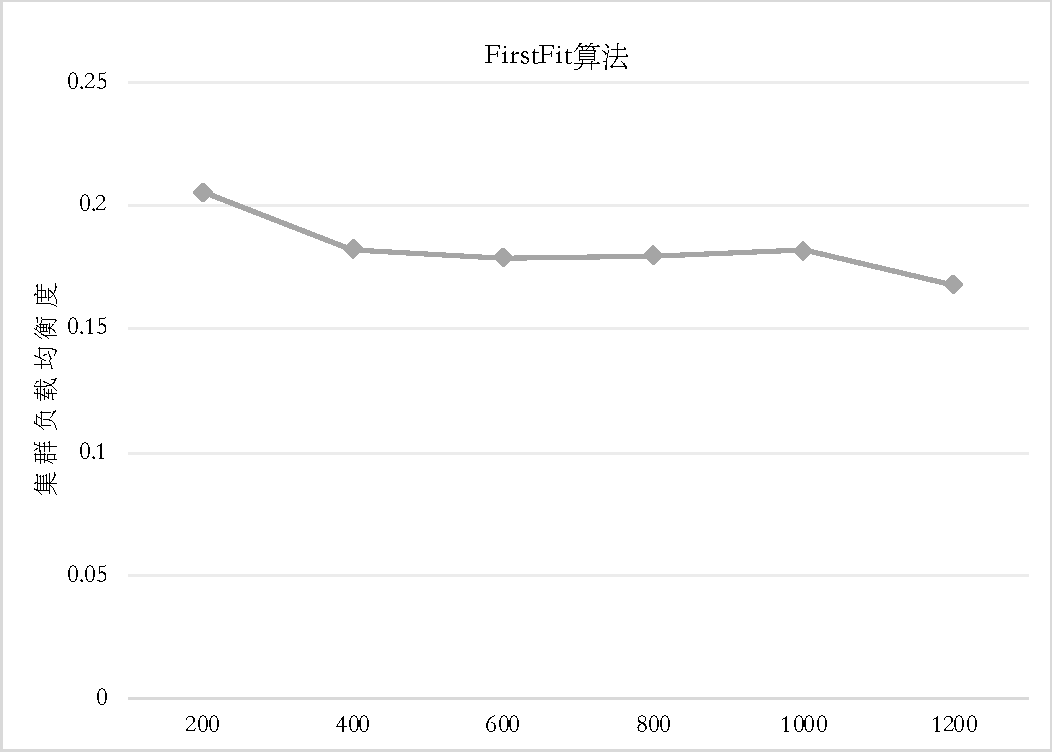
\includegraphics[width=7cm,height=5cm]{firstfit-cluster}
		\caption{FirstFit算法节点负载均衡度}
	\end{subfigure}%
	\hspace{0.5cm}%
	\begin{subfigure}{7cm}
		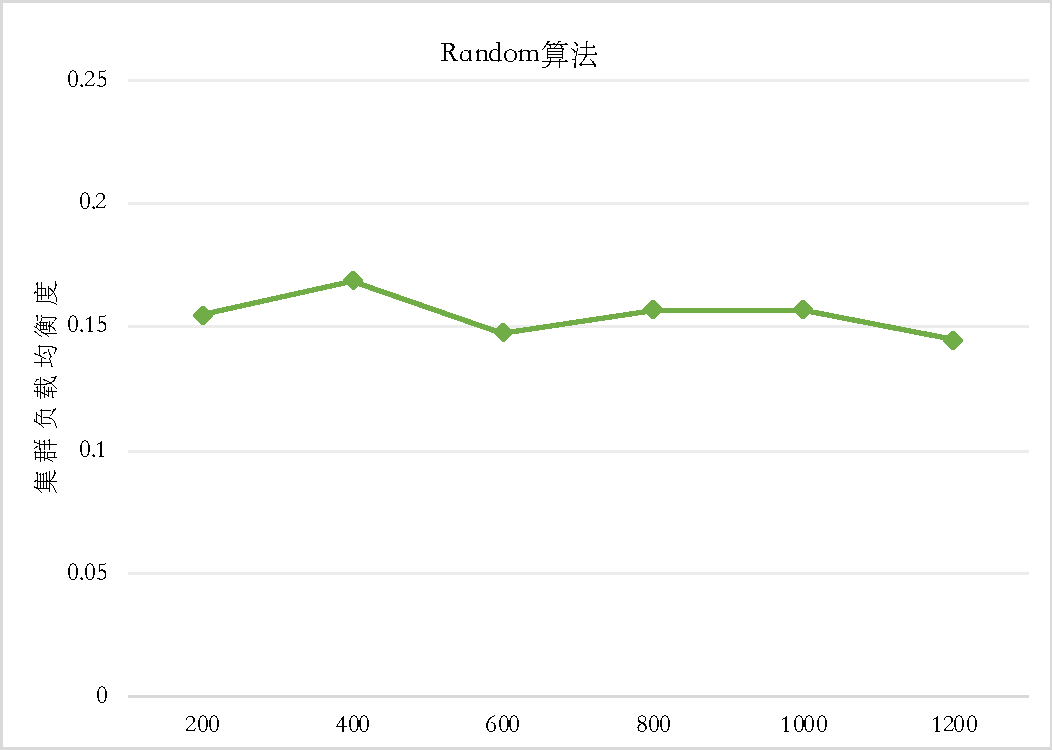
\includegraphics[width=7cm, height=5cm]{random-cluster}
		\centering{\caption{Random算法节点负载均衡度}}
	\end{subfigure}
	\begin{subfigure}{7cm}
		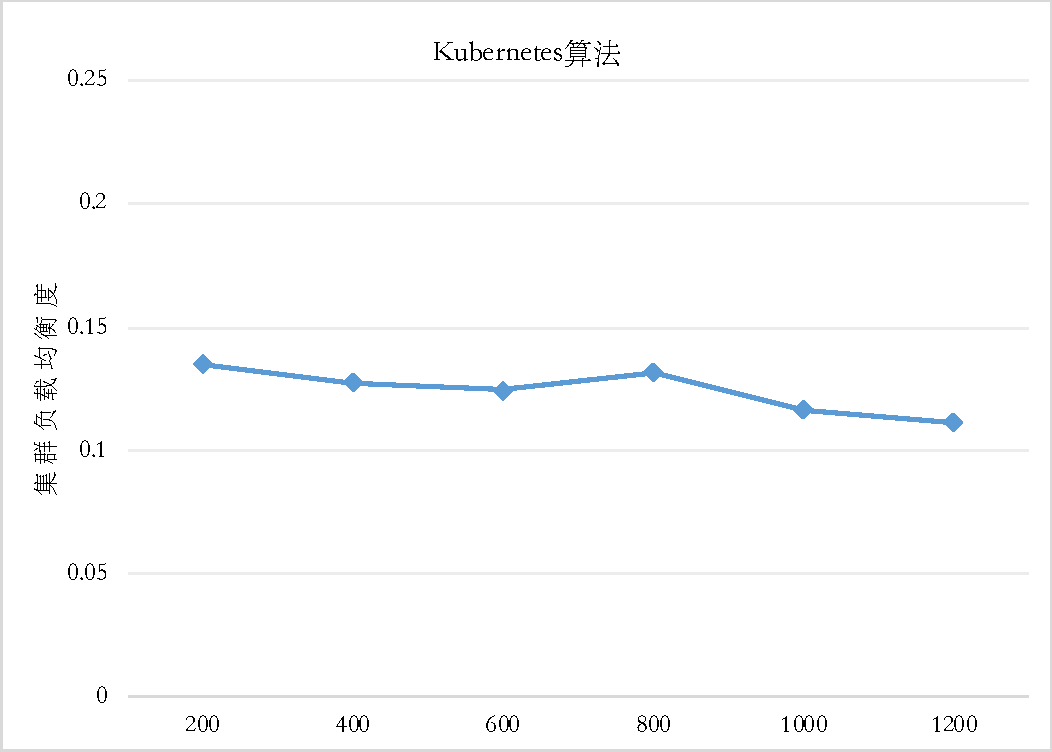
\includegraphics[width=7cm,height=5cm]{kub-cluster}
		\caption{kubernetes节点负载均衡度}
	\end{subfigure}%
	\hspace{0.5cm}%
	\begin{subfigure}{7cm}
		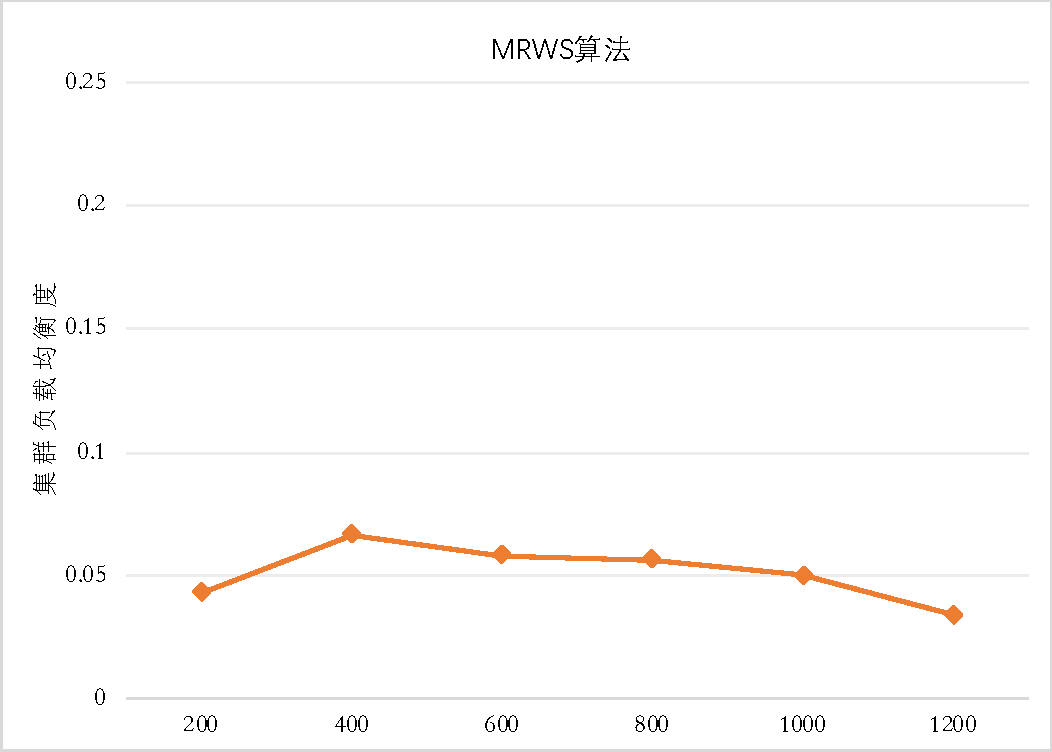
\includegraphics[width=7cm, height=5cm]{mrws-cluster}
		\centering{\caption{MRWS算法节点负载均衡度}}
	\end{subfigure}
	\caption{四种调度算法下集群负载均衡度}	
\end{figure}

如图5.6所示,MRWS调度算法集群的负载均衡度最小,大概为Kubernetes算法的二分之一,Ramdom和FirstFit算法的四分之一。因此,在MRWS调度算法的集群中各节点资源消耗情况趋于均衡,单个节点上各维度资源利用也较为均衡,集群的服务性能更优秀。针对集群的服务性能将使用多计算框架应用混合部署在实际的实验平台上进行测试,测试集中调度算方法下混合应用的完成时间。

\section{Paladin容器云平台部署}

























\chapter{总结与展望}
本文在进行“多元化大数据高效能存储与处理”项目研究时,发现在面向多计算框架的容器云平台Paladin上进行多计算框架容器应用混合部署下集群性能较低。Paladin的服务层是基于开源OpenShift Origin容器云平台构建,而OpenShift Origin的容器编排引擎是Kubernetes。接着对主流的容器编排引擎Kubernetes、Mesos以及Docker Swarm进行分析,尤其针对Kubernetes的调度流程和调度算法进行深入研究,发现其调度流程不够优化,并且调度算法在评分阶段仅考虑内存和CPU的空闲率平衡情况,导致其他维度资源利用率不足和负载不均衡,从而使集群效率低下。针对其调度方案不足,本文首先优化其调度流程,通过一个Hash表管理重复部署的容器应用,避免镜像重复下载,节约磁盘和网络资源。

针对Kubernetes容器调度算法不足,本文提出一个基于多维资源权重参数的调度方案MRWS,该方法综合考虑集群中节点CPU、内存、磁盘、网络带宽和已部署Pod数量等因素,赋予每个影响调度因子一个权重值进行综合评分。权重参数根据容器应用对资源的需求和节点资源空闲率进行建模,使用模糊层次分析法FAHP自动构建模糊成对比矩阵和判断矩阵,计算出满足一致性要求的权重参数作为待调度容器应用各维度资源的权重值。对于新提出的调度算法,在容器云仿真平台ContainerCloudSim上进行大规模调度仿真,并与Kubernetes、Random、FirstFIt调度算法在集群资源利用率和负载均衡度方面进行对比。最后在大数据存储与处的理容器云Paladin平台上实际开发调度方案,进行多计算框架混合部署实际调度性能测试。实验表明新的调度算法无论在单计算框架容器应用执行效率还是同时运行多计算框架容器应用执行效率方面都有较大的提升。

总体而言,本文主要围绕面向多计算框架的容器云平台Paladin上多计算框架容器应用混合部署下执行效率过低的问题做了以下几个方面工作:
\begin{enumerate}[(1)]
	\item 调研当前容器编排引擎集中式调度、两层调度和共享状态调度模型的典型架构,并以实际例子分析各自的优缺点。深入分析Kubernetes调度流程和算法不足,对其调度流程进行优化并提出了一种新的综合考虑容器应用CPU、内存、磁盘、网络带宽以及已部署Pod等因素的调度方案MRWS。
	\item 针对调度方案MRWS中多维资源权重问题,使用模糊层次分析法自动建模和构建满足一致性要求的模糊成对比矩阵和判断矩阵,实现新的调度方案。
	\item 在容器云仿真平台ContainerCloudSim上针对新的调度方案进行大规模调度仿真,并与常见的Random、FirstFit以及Kubernetes默认的Default调度方案进行资源利用率和负载均衡度对比。
	\item 在Paladin容器云平台上构建数十种多计算框架,用户可以实现快速构建大数据处理环境和容器伸缩。接着开发新的调度方案MRWS,并在该平台上进行多计算框架混合部署,测试对比几种调度算法的性能,实验表明新的调度方案极大提升了集群的服务性能,缩短多计算框架任务的执行时间。
\end{enumerate}

本文主要围绕提升面向多计算框架的容器云平台Paladin服务性能开展研究工作,容器资源调度是提升容器云集群的关键因素,要使一个容器云平台具有更好的性能,在后续的研究工作中可以从以下几个方面进行:
\begin{enumerate}[1.]
	\item 数据亲和性调度。Paladin是一个集大数据存储与处理于一身的容器云平台,底层是一个分布式的文件系统,通过客户端磁盘挂载形式实现数据访问,并提供web-console的大数据上传、下载、删除、修改等管理操作。因此,在数据处理框架进行数据处理时,数据的位置对其性能存在重大影响,需要研究以数据为中心的调度方案,实现数据亲和性调度,将数据存储和处理容器尽可能调度到相同或近距离的节点,减少网络传输和磁盘I/O。
	\item 优先抢占式调度。在大数据批处理中有的任务无需及时处理,如Hadoop进行离线数据处理,有的需要进行及时快速地处理如流计算等。调度系统需要实现优先抢占式调度,在紧急任务模式下暂停优先级较低的任务,给予优先级高任务更多的计算资源。
	\item 容器迁移策略研究。多计算框架混合部署场景下资源的分配是静态的,有的用户在部署完计算框架后并不进行任务处理。根据这一特点可以实现集群资源超卖,在保证性能情况下实现经济利益最大化。一些不太活跃用户的容器可以迁移到性能较低的节点上,在用户使用时再迁回高性能的节点。
	\item 任务特征调度。根据积累数据中心的数据提取更多用户计算框架处理任务的特征,根据特征制定合适的调度方案,最大化的利用集群的资源。让集群调度更加智能,实现按需服务,提升用户的服务体验。
\end{enumerate}
%%% 其它部分
\backmatter

%% 本科生要这几个索引,研究生不要。选择性留下。
% 插图索引
%\listoffigures
% 表格索引
%\listoftables
% 公式索引
%\listofequations


%% 参考文献
% 注意:至少需要引用一篇参考文献,否则下面两行可能引起编译错误。
% 如果不需要参考文献,请将下面两行删除或注释掉。
% 数字式引用
\bibliographystyle{thuthesis-numeric}
% 作者-年份式引用
% \bibliographystyle{thuthesis-author-year}
\bibliography{ref/refs}


%% 致谢
% 如果使用声明扫描页,将可选参数指定为扫描后的 PDF 文件名,例如:
% \begin{acknowledgement}[scan-statement.pdf]
\begin{acknowledgement}
	光阴似箭,岁月如流水,转眼已在园子里度过了三年时光,在三年硕士期间,老师们的谆谆教诲,同学们的热情帮助,让我不仅在学业上进步,也让我度过人生中一段快乐的时光。
	
	首先我要感谢我的导师武永卫教授在硕士三年期间不但给予学术上的指导,在生活上也给予了悉心的照顾,更教会了我许多做人的道理。武老师是一个和蔼可亲的人,他治理下的实验室宽松、活跃以及浓厚的学术氛围让我收获颇丰。其次要由衷感谢陈康副教授和姜进磊副教授,陈康老师不仅与学生亦师亦友,更是一位计算机的百科全书,他知识面广而深,对待问题较真的态度影响实验室的每一个人,在我小论文投稿方面给予了很多指导。再次感谢三位老师在硕士期间给予的指导和帮助,祝各位老师阖家幸福!
	
	其次我要感谢实验室同学的照顾,艾志远是第一个给予我指导和帮助的师兄,他工程能力极强,对我帮助很大。马腾、刘梦醒、杨珂、李雪、夏鑫、李志涛、何东标等实验室的同学不仅让我感受到Madsys实验室的温暖,也常常帮我答疑解惑,与大家在一起的时光很开心,衷心祝愿大家学业进步,事业有成!
	
	最后我要感谢我的父母和女朋友,你们在我困惑和无助的时候给予我很大鼓励和安慰,一直在背后默默的付出和支持我。感谢你们辛勤的付出和关爱,让我能够在硕士期间安心完成学业,你们的爱是我前进的不竭动力。谨向所有在我硕士期间帮助我和指导我的老师、同学、朋友表示衷心的感谢!
	
\end{acknowledgement}


%% 附录
%\begin{appendix}
%\chapter{外文资料原文}
\label{cha:engorg}

\title{The title of the English paper}

\textbf{Abstract:} As one of the most widely used techniques in operations
research, \emph{ mathematical programming} is defined as a means of maximizing a
quantity known as \emph{bjective function}, subject to a set of constraints
represented by equations and inequalities. Some known subtopics of mathematical
programming are linear programming, nonlinear programming, multiobjective
programming, goal programming, dynamic programming, and multilevel
programming$^{[1]}$.

It is impossible to cover in a single chapter every concept of mathematical
programming. This chapter introduces only the basic concepts and techniques of
mathematical programming such that readers gain an understanding of them
throughout the book$^{[2,3]}$.


\section{Single-Objective Programming}
The general form of single-objective programming (SOP) is written
as follows,
\begin{equation}\tag*{(123)} % 如果附录中的公式不想让它出现在公式索引中,那就请
                             % 用 \tag*{xxxx}
\left\{\begin{array}{l}
\max \,\,f(x)\\[0.1 cm]
\mbox{subject to:} \\ [0.1 cm]
\qquad g_j(x)\le 0,\quad j=1,2,\cdots,p
\end{array}\right.
\end{equation}
which maximizes a real-valued function $f$ of
$x=(x_1,x_2,\cdots,x_n)$ subject to a set of constraints.

\newtheorem{mpdef}{Definition}[chapter]
\begin{mpdef}
In SOP, we call $x$ a decision vector, and
$x_1,x_2,\cdots,x_n$ decision variables. The function
$f$ is called the objective function. The set
\begin{equation}\tag*{(456)} % 这里同理,其它不再一一指定。
S=\left\{x\in\Re^n\bigm|g_j(x)\le 0,\,j=1,2,\cdots,p\right\}
\end{equation}
is called the feasible set. An element $x$ in $S$ is called a
feasible solution.
\end{mpdef}

\newtheorem{mpdefop}[mpdef]{Definition}
\begin{mpdefop}
A feasible solution $x^*$ is called the optimal
solution of SOP if and only if
\begin{equation}
f(x^*)\ge f(x)
\end{equation}
for any feasible solution $x$.
\end{mpdefop}

One of the outstanding contributions to mathematical programming was known as
the Kuhn-Tucker conditions\ref{eq:ktc}. In order to introduce them, let us give
some definitions. An inequality constraint $g_j(x)\le 0$ is said to be active at
a point $x^*$ if $g_j(x^*)=0$. A point $x^*$ satisfying $g_j(x^*)\le 0$ is said
to be regular if the gradient vectors $\nabla g_j(x)$ of all active constraints
are linearly independent.

Let $x^*$ be a regular point of the constraints of SOP and assume that all the
functions $f(x)$ and $g_j(x),j=1,2,\cdots,p$ are differentiable. If $x^*$ is a
local optimal solution, then there exist Lagrange multipliers
$\lambda_j,j=1,2,\cdots,p$ such that the following Kuhn-Tucker conditions hold,
\begin{equation}
\label{eq:ktc}
\left\{\begin{array}{l}
    \nabla f(x^*)-\sum\limits_{j=1}^p\lambda_j\nabla g_j(x^*)=0\\[0.3cm]
    \lambda_jg_j(x^*)=0,\quad j=1,2,\cdots,p\\[0.2cm]
    \lambda_j\ge 0,\quad j=1,2,\cdots,p.
\end{array}\right.
\end{equation}
If all the functions $f(x)$ and $g_j(x),j=1,2,\cdots,p$ are convex and
differentiable, and the point $x^*$ satisfies the Kuhn-Tucker conditions
(\ref{eq:ktc}), then it has been proved that the point $x^*$ is a global optimal
solution of SOP.

\subsection{Linear Programming}
\label{sec:lp}

If the functions $f(x),g_j(x),j=1,2,\cdots,p$ are all linear, then SOP is called
a {\em linear programming}.

The feasible set of linear is always convex. A point $x$ is called an extreme
point of convex set $S$ if $x\in S$ and $x$ cannot be expressed as a convex
combination of two points in $S$. It has been shown that the optimal solution to
linear programming corresponds to an extreme point of its feasible set provided
that the feasible set $S$ is bounded. This fact is the basis of the {\em simplex
  algorithm} which was developed by Dantzig as a very efficient method for
solving linear programming.
\begin{table}[ht]
\centering
  \centering
  \caption*{Table~1\hskip1em This is an example for manually numbered table, which
    would not appear in the list of tables}
  \label{tab:badtabular2}
  \begin{tabular}[c]{|m{1.5cm}|c|c|c|c|c|c|}\hline
    \multicolumn{2}{|c|}{Network Topology} & \# of nodes &
    \multicolumn{3}{c|}{\# of clients} & Server \\\hline
    GT-ITM & Waxman Transit-Stub & 600 &
    \multirow{2}{2em}{2\%}&
    \multirow{2}{2em}{10\%}&
    \multirow{2}{2em}{50\%}&
    \multirow{2}{1.2in}{Max. Connectivity}\\\cline{1-3}
    \multicolumn{2}{|c|}{Inet-2.1} & 6000 & & & &\\\hline
    \multirow{2}{1.5cm}{Xue} & Rui  & Ni &\multicolumn{4}{c|}{\multirow{2}*{\thuthesis}}\\\cline{2-3}
    & \multicolumn{2}{c|}{ABCDEF} &\multicolumn{4}{c|}{} \\\hline
\end{tabular}
\end{table}

Roughly speaking, the simplex algorithm examines only the extreme points of the
feasible set, rather than all feasible points. At first, the simplex algorithm
selects an extreme point as the initial point. The successive extreme point is
selected so as to improve the objective function value. The procedure is
repeated until no improvement in objective function value can be made. The last
extreme point is the optimal solution.

\subsection{Nonlinear Programming}

If at least one of the functions $f(x),g_j(x),j=1,2,\cdots,p$ is nonlinear, then
SOP is called a {\em nonlinear programming}.

A large number of classical optimization methods have been developed to treat
special-structural nonlinear programming based on the mathematical theory
concerned with analyzing the structure of problems.
\begin{figure}[h]
  \centering
  
\includegraphics{thu-lib-logo}
  \caption*{Figure~1\quad This is an example for manually numbered figure,
    which would not appear in the list of figures}
  \label{tab:badfigure2}
\end{figure}

Now we consider a nonlinear programming which is confronted solely with
maximizing a real-valued function with domain $\Re^n$.  Whether derivatives are
available or not, the usual strategy is first to select a point in $\Re^n$ which
is thought to be the most likely place where the maximum exists. If there is no
information available on which to base such a selection, a point is chosen at
random. From this first point an attempt is made to construct a sequence of
points, each of which yields an improved objective function value over its
predecessor. The next point to be added to the sequence is chosen by analyzing
the behavior of the function at the previous points. This construction continues
until some termination criterion is met. Methods based upon this strategy are
called {\em ascent methods}, which can be classified as {\em direct methods},
{\em gradient methods}, and {\em Hessian methods} according to the information
about the behavior of objective function $f$. Direct methods require only that
the function can be evaluated at each point. Gradient methods require the
evaluation of first derivatives of $f$. Hessian methods require the evaluation
of second derivatives. In fact, there is no superior method for all
problems. The efficiency of a method is very much dependent upon the objective
function.

\subsection{Integer Programming}

{\em Integer programming} is a special mathematical programming in which all of
the variables are assumed to be only integer values. When there are not only
integer variables but also conventional continuous variables, we call it {\em
  mixed integer programming}. If all the variables are assumed either 0 or 1,
then the problem is termed a {\em zero-one programming}. Although integer
programming can be solved by an {\em exhaustive enumeration} theoretically, it
is impractical to solve realistically sized integer programming problems. The
most successful algorithm so far found to solve integer programming is called
the {\em branch-and-bound enumeration} developed by Balas (1965) and Dakin
(1965). The other technique to integer programming is the {\em cutting plane
  method} developed by Gomory (1959).

\hfill\textit{Uncertain Programming\/}\quad(\textsl{BaoDing Liu, 2006.2})

\section*{References}
\noindent{\itshape NOTE: These references are only for demonstration. They are
  not real citations in the original text.}

\begin{translationbib}
\item Donald E. Knuth. The \TeX book. Addison-Wesley, 1984. ISBN: 0-201-13448-9
\item Paul W. Abrahams, Karl Berry and Kathryn A. Hargreaves. \TeX\ for the
  Impatient. Addison-Wesley, 1990. ISBN: 0-201-51375-7
\item David Salomon. The advanced \TeX book.  New York : Springer, 1995. ISBN:0-387-94556-3
\end{translationbib}

\chapter{外文资料的调研阅读报告或书面翻译}

\title{英文资料的中文标题}

{\heiti 摘要:} 本章为外文资料翻译内容。如果有摘要可以直接写上来,这部分好像没有
明确的规定。

\section{单目标规划}
北冥有鱼,其名为鲲。鲲之大,不知其几千里也。化而为鸟,其名为鹏。鹏之背,不知其几
千里也。怒而飞,其翼若垂天之云。是鸟也,海运则将徙于南冥。南冥者,天池也。
\begin{equation}\tag*{(123)}
 p(y|\mathbf{x}) = \frac{p(\mathbf{x},y)}{p(\mathbf{x})}=
\frac{p(\mathbf{x}|y)p(y)}{p(\mathbf{x})}
\end{equation}

吾生也有涯,而知也无涯。以有涯随无涯,殆已!已而为知者,殆而已矣!为善无近名,为
恶无近刑,缘督以为经,可以保身,可以全生,可以养亲,可以尽年。

\subsection{线性规划}
庖丁为文惠君解牛,手之所触,肩之所倚,足之所履,膝之所倚,砉然响然,奏刀騞然,莫
不中音,合于桑林之舞,乃中经首之会。
\begin{table}[ht]
\centering
  \centering
  \caption*{表~1\hskip1em 这是手动编号但不出现在索引中的一个表格例子}
  \label{tab:badtabular3}
  \begin{tabular}[c]{|m{1.5cm}|c|c|c|c|c|c|}\hline
    \multicolumn{2}{|c|}{Network Topology} & \# of nodes &
    \multicolumn{3}{c|}{\# of clients} & Server \\\hline
    GT-ITM & Waxman Transit-Stub & 600 &
    \multirow{2}{2em}{2\%}&
    \multirow{2}{2em}{10\%}&
    \multirow{2}{2em}{50\%}&
    \multirow{2}{1.2in}{Max. Connectivity}\\\cline{1-3}
    \multicolumn{2}{|c|}{Inet-2.1} & 6000 & & & &\\\hline
    \multirow{2}{1.5cm}{Xue} & Rui  & Ni &\multicolumn{4}{c|}{\multirow{2}*{\thuthesis}}\\\cline{2-3}
    & \multicolumn{2}{c|}{ABCDEF} &\multicolumn{4}{c|}{} \\\hline
\end{tabular}
\end{table}

文惠君曰:“嘻,善哉!技盖至此乎?”庖丁释刀对曰:“臣之所好者道也,进乎技矣。始臣之
解牛之时,所见无非全牛者;三年之后,未尝见全牛也;方今之时,臣以神遇而不以目视,
官知止而神欲行。依乎天理,批大郤,导大窾,因其固然。技经肯綮之未尝,而况大坬乎!
良庖岁更刀,割也;族庖月更刀,折也;今臣之刀十九年矣,所解数千牛矣,而刀刃若新发
于硎。彼节者有间而刀刃者无厚,以无厚入有间,恢恢乎其于游刃必有余地矣。是以十九年
而刀刃若新发于硎。虽然,每至于族,吾见其难为,怵然为戒,视为止,行为迟,动刀甚微,
謋然已解,如土委地。提刀而立,为之而四顾,为之踌躇满志,善刀而藏之。”

文惠君曰:“善哉!吾闻庖丁之言,得养生焉。”


\subsection{非线性规划}
孔子与柳下季为友,柳下季之弟名曰盗跖。盗跖从卒九千人,横行天下,侵暴诸侯。穴室枢
户,驱人牛马,取人妇女。贪得忘亲,不顾父母兄弟,不祭先祖。所过之邑,大国守城,小
国入保,万民苦之。孔子谓柳下季曰:“夫为人父者,必能诏其子;为人兄者,必能教其弟。
若父不能诏其子,兄不能教其弟,则无贵父子兄弟之亲矣。今先生,世之才士也,弟为盗
跖,为天下害,而弗能教也,丘窃为先生羞之。丘请为先生往说之。”
\begin{figure}[h]
  \centering
  
\includegraphics{thu-whole-logo}
  \caption*{图~1\hskip1em 这是手动编号但不出现索引中的图片的例子}
  \label{tab:badfigure3}
\end{figure}

柳下季曰:“先生言为人父者必能诏其子,为人兄者必能教其弟,若子不听父之诏,弟不受
兄之教,虽今先生之辩,将奈之何哉?且跖之为人也,心如涌泉,意如飘风,强足以距敌,
辩足以饰非。顺其心则喜,逆其心则怒,易辱人以言。先生必无往。”

孔子不听,颜回为驭,子贡为右,往见盗跖。

\subsection{整数规划}
盗跖乃方休卒徒大山之阳,脍人肝而餔之。孔子下车而前,见谒者曰:“鲁人孔丘,闻将军
高义,敬再拜谒者。”谒者入通。盗跖闻之大怒,目如明星,发上指冠,曰:“此夫鲁国之
巧伪人孔丘非邪?为我告之:尔作言造语,妄称文、武,冠枝木之冠,带死牛之胁,多辞缪
说,不耕而食,不织而衣,摇唇鼓舌,擅生是非,以迷天下之主,使天下学士不反其本,妄
作孝弟,而侥幸于封侯富贵者也。子之罪大极重,疾走归!不然,我将以子肝益昼餔之膳。”


\chapter{其它附录}
前面两个附录主要是给本科生做例子。其它附录的内容可以放到这里,当然如果你愿意,可
以把这部分也放到独立的文件中,然后将其 \cs{input} 到主文件中。

%\end{appendix}

%% 个人简历
\begin{resume}

  \resumeitem{个人简历}

 1991 年 04 月 27 日出生于 贵州 省 铜仁 市。

  2010 年 9 月考入 清华 大学 计算机 系 ,2014 年 7 月本科毕业并获得 工 学士学位。

  2016 年 9 月免试进入 清华 大学 计算机 系攻读 硕士 学位至今。

\researchitem{发表的学术论文} % 发表的和录用的合在一起

% 1. 已经刊载的学术论文(本人是第一作者,或者导师为第一作者本人是第二作者)
\begin{publications}
	\item 龚坤, 武永卫, 陈康, 等. 容器云多维资源利用率均衡调度研究. 计算机应用研究(已被录用, 2020第37卷第4期)
\end{publications}

\end{resume}


%% 本科生进行格式审查是需要下面这个表格,答辩可能不需要。选择性留下。
% 综合论文训练记录表
%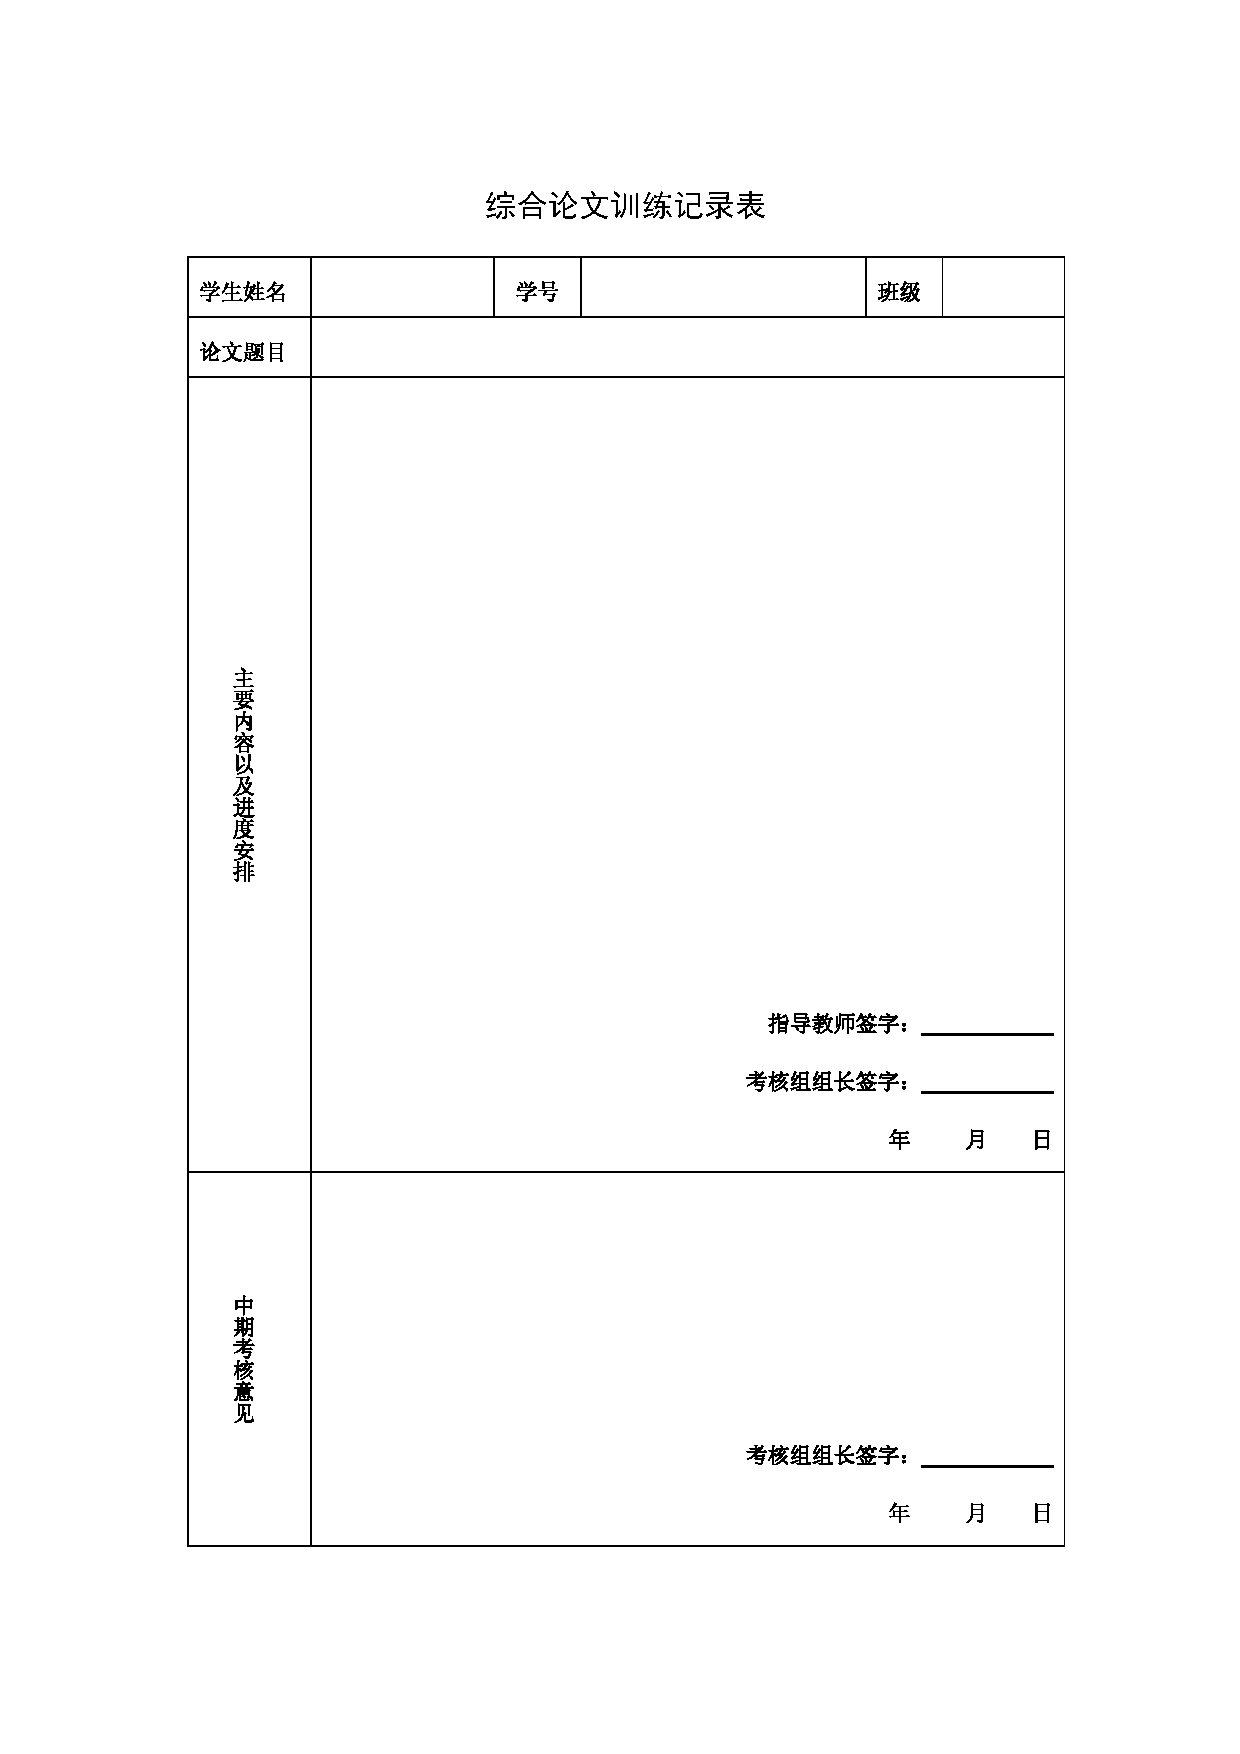
\includepdf[pages=-]{scan-record.pdf}
\end{document}
